% Options for packages loaded elsewhere
% Options for packages loaded elsewhere
\PassOptionsToPackage{unicode}{hyperref}
\PassOptionsToPackage{hyphens}{url}
\PassOptionsToPackage{dvipsnames,svgnames,x11names}{xcolor}
\PassOptionsToPackage{space}{xeCJK}
%
\documentclass[
  chinese,
  letterpaper,
  DIV=11,
  numbers=noendperiod]{scrreprt}
\usepackage{xcolor}
\usepackage{amsmath,amssymb}
\setcounter{secnumdepth}{5}
\usepackage{iftex}
\ifPDFTeX
  \usepackage[T1]{fontenc}
  \usepackage[utf8]{inputenc}
  \usepackage{textcomp} % provide euro and other symbols
\else % if luatex or xetex
  \usepackage{unicode-math} % this also loads fontspec
  \defaultfontfeatures{Scale=MatchLowercase}
  \defaultfontfeatures[\rmfamily]{Ligatures=TeX,Scale=1}
\fi
\usepackage{lmodern}
\ifPDFTeX\else
  % xetex/luatex font selection
  \setmainfont[]{Noto Serif TC}
  \setsansfont[]{Noto Serif TC}
  \ifXeTeX
    \usepackage{xeCJK}
    \setCJKmainfont[]{Noto Serif TC}
  \fi
  \ifLuaTeX
    \usepackage[]{luatexja-fontspec}
    \setmainjfont[]{Noto Serif TC}
  \fi
\fi
% Use upquote if available, for straight quotes in verbatim environments
\IfFileExists{upquote.sty}{\usepackage{upquote}}{}
\IfFileExists{microtype.sty}{% use microtype if available
  \usepackage[]{microtype}
  \UseMicrotypeSet[protrusion]{basicmath} % disable protrusion for tt fonts
}{}
\makeatletter
\@ifundefined{KOMAClassName}{% if non-KOMA class
  \IfFileExists{parskip.sty}{%
    \usepackage{parskip}
  }{% else
    \setlength{\parindent}{0pt}
    \setlength{\parskip}{6pt plus 2pt minus 1pt}}
}{% if KOMA class
  \KOMAoptions{parskip=half}}
\makeatother
% Make \paragraph and \subparagraph free-standing
\makeatletter
\ifx\paragraph\undefined\else
  \let\oldparagraph\paragraph
  \renewcommand{\paragraph}{
    \@ifstar
      \xxxParagraphStar
      \xxxParagraphNoStar
  }
  \newcommand{\xxxParagraphStar}[1]{\oldparagraph*{#1}\mbox{}}
  \newcommand{\xxxParagraphNoStar}[1]{\oldparagraph{#1}\mbox{}}
\fi
\ifx\subparagraph\undefined\else
  \let\oldsubparagraph\subparagraph
  \renewcommand{\subparagraph}{
    \@ifstar
      \xxxSubParagraphStar
      \xxxSubParagraphNoStar
  }
  \newcommand{\xxxSubParagraphStar}[1]{\oldsubparagraph*{#1}\mbox{}}
  \newcommand{\xxxSubParagraphNoStar}[1]{\oldsubparagraph{#1}\mbox{}}
\fi
\makeatother


\usepackage{longtable,booktabs,array}
\usepackage{calc} % for calculating minipage widths
% Correct order of tables after \paragraph or \subparagraph
\usepackage{etoolbox}
\makeatletter
\patchcmd\longtable{\par}{\if@noskipsec\mbox{}\fi\par}{}{}
\makeatother
% Allow footnotes in longtable head/foot
\IfFileExists{footnotehyper.sty}{\usepackage{footnotehyper}}{\usepackage{footnote}}
\makesavenoteenv{longtable}
\usepackage{graphicx}
\makeatletter
\newsavebox\pandoc@box
\newcommand*\pandocbounded[1]{% scales image to fit in text height/width
  \sbox\pandoc@box{#1}%
  \Gscale@div\@tempa{\textheight}{\dimexpr\ht\pandoc@box+\dp\pandoc@box\relax}%
  \Gscale@div\@tempb{\linewidth}{\wd\pandoc@box}%
  \ifdim\@tempb\p@<\@tempa\p@\let\@tempa\@tempb\fi% select the smaller of both
  \ifdim\@tempa\p@<\p@\scalebox{\@tempa}{\usebox\pandoc@box}%
  \else\usebox{\pandoc@box}%
  \fi%
}
% Set default figure placement to htbp
\def\fps@figure{htbp}
\makeatother



\ifLuaTeX
\usepackage[bidi=basic,provide=*]{babel}
\else
\usepackage[bidi=default,provide=*]{babel}
\fi
\ifPDFTeX
\else
\babelfont{rm}[]{Noto Serif TC}
\fi
% get rid of language-specific shorthands (see #6817):
\let\LanguageShortHands\languageshorthands
\def\languageshorthands#1{}


\setlength{\emergencystretch}{3em} % prevent overfull lines

\providecommand{\tightlist}{%
  \setlength{\itemsep}{0pt}\setlength{\parskip}{0pt}}



 


\KOMAoption{captions}{tableheading}
\usepackage{float}
\usepackage{zhnumber}
\renewcommand\partformat{第\zhnum{part}篇\enskip}
\renewcommand\chapterformat{第\zhnum{chapter}章\enskip}
\makeatletter
\@ifpackageloaded{bookmark}{}{\usepackage{bookmark}}
\makeatother
\makeatletter
\@ifpackageloaded{caption}{}{\usepackage{caption}}
\AtBeginDocument{%
\ifdefined\contentsname
  \renewcommand*\contentsname{目錄}
\else
  \newcommand\contentsname{目錄}
\fi
\ifdefined\listfigurename
  \renewcommand*\listfigurename{圖目錄}
\else
  \newcommand\listfigurename{圖目錄}
\fi
\ifdefined\listtablename
  \renewcommand*\listtablename{表目錄}
\else
  \newcommand\listtablename{表目錄}
\fi
\ifdefined\figurename
  \renewcommand*\figurename{圖}
\else
  \newcommand\figurename{圖}
\fi
\ifdefined\tablename
  \renewcommand*\tablename{表}
\else
  \newcommand\tablename{表}
\fi
}
\@ifpackageloaded{float}{}{\usepackage{float}}
\floatstyle{ruled}
\@ifundefined{c@chapter}{\newfloat{codelisting}{h}{lop}}{\newfloat{codelisting}{h}{lop}[chapter]}
\floatname{codelisting}{列表}
\newcommand*\listoflistings{\listof{codelisting}{列表目錄}}
\makeatother
\makeatletter
\makeatother
\makeatletter
\@ifpackageloaded{caption}{}{\usepackage{caption}}
\@ifpackageloaded{subcaption}{}{\usepackage{subcaption}}
\makeatother
\usepackage{bookmark}
\IfFileExists{xurl.sty}{\usepackage{xurl}}{} % add URL line breaks if available
\urlstyle{same}
\hypersetup{
  pdftitle={AI 應用規劃師全攻略},
  pdfauthor={AI仁波切},
  pdflang={zh-TW},
  colorlinks=true,
  linkcolor={blue},
  filecolor={Maroon},
  citecolor={Blue},
  urlcolor={Blue},
  pdfcreator={LaTeX via pandoc}}


\title{AI 應用規劃師全攻略}
\author{AI仁波切}
\date{2025-11-20}
\begin{document}
\maketitle

\renewcommand*\contentsname{目錄}
{
\hypersetup{linkcolor=}
\setcounter{tocdepth}{2}
\tableofcontents
}

\bookmarksetup{startatroot}

\part{人工智慧應用規劃與基礎理論全書}\label{ux4ebaux5de5ux667aux6167ux61c9ux7528ux898fux5283ux8207ux57faux790eux7406ux8ad6ux5168ux66f8}

\bookmarksetup{startatroot}

\part*{前言}\label{ux524dux8a00}
\addcontentsline{toc}{part}{前言}

\markboth{前言}{前言}

\textbf{適用對象：} 準備經濟部 iPAS AI
應用規劃師（初/中級）及資策會人工智慧工程素養認證之考生。

本攻略旨在協助考生掌握 AI 應用規劃師與工程素養認證之核心知識，
內容涵蓋人工智慧基礎、 機器學習、 深度學習、 生成式 AI、 大數據分析、 AI
倫理與法規， 以及 Python 程式語言基礎。

請點選左側目錄開始閱讀各章節。

\part{第一部：人工智慧基礎與戰略定位}

\part{人工智慧的本質與層次架構}\label{ux4ebaux5de5ux667aux6167ux7684ux672cux8ceaux8207ux5c64ux6b21ux67b6ux69cb}

人工智慧 (Artificial Intelligence, AI)
已經成為當今科技發展的核心驅動力，深刻地改變著我們的生活與工作方式。本章將帶領讀者深入探討
AI 的定義、技術層次架構，以及人類與 AI
之間多樣化的協作模式，為後續的學習奠定堅實的基礎。

\chapter{1.1 AI
的定義與範疇}\label{ai-ux7684ux5b9aux7fa9ux8207ux7bc4ux7587}

\section{人工智慧 (Artificial Intelligence, AI) 定義}\label{sec-ai-def}

人工智慧 (AI)
是一個廣泛的學科，旨在創造能夠展現「智慧」行為的機器或軟體。簡單來說，AI
就是讓電腦具備模擬人類認知功能的能力，例如學習、推理、解決問題、感知環境、理解語言等。

AI
的目標並非僅僅是模仿人類，更在於透過計算能力來增強人類的智慧，解決複雜的問題。從早期的邏輯推理程式到現在的生成式
AI，AI 的定義隨著技術的演進而不斷擴展。

\section{弱 AI (Narrow AI) vs.~強 AI (General
AI/AGI)}\label{ux5f31-ai-narrow-ai-vs.-ux5f37-ai-general-aiagi}

根據 AI 的能力範圍，我們可以將其分為兩大類：

\begin{enumerate}
\def\labelenumi{\arabic{enumi}.}
\tightlist
\item
  \textbf{弱人工智慧 (Artificial Narrow Intelligence, ANI)}
  \{\#def-ani\}：

  \begin{itemize}
  \tightlist
  \item
    \textbf{定義}：又稱為「專用 AI」。這類 AI
    專精於執行「單一」或「特定」的任務，且在該領域的表現可能超越人類。目前我們生活中所見到的
    AI 幾乎都屬於此類。
  \item
    \textbf{特徵}：不具備自我意識，無法跨領域學習。它的智慧是「被設計」出來解決特定問題的。
  \item
    \textbf{例子}：

    \begin{itemize}
    \tightlist
    \item
      \textbf{AlphaGo}：雖然圍棋下得比世界冠軍好，但它不會開車，也不會聊天。
    \item
      \textbf{Siri / Google
      Assistant}：能聽懂語音指令，但無法理解複雜的情感或進行深度的哲學思考。
    \item
      \textbf{人臉辨識系統}：能精準辨識身分，但無法欣賞照片的美感。
    \end{itemize}
  \end{itemize}
\item
  \textbf{強人工智慧 (Artificial General Intelligence, AGI)}
  \{\#def-agi\}：

  \begin{itemize}
  \tightlist
  \item
    \textbf{定義}：又稱為「通用 AI」。這類 AI
    具備像人類一樣的「通用智慧」，能夠像人類一樣學習任何智力任務。它具備常識、推理能力、情感理解，甚至自我意識。
  \item
    \textbf{特徵}：能夠跨領域遷移學習，面對未曾見過的問題也能嘗試解決。
  \item
    \textbf{現狀}：目前仍處於理論和研發階段，尚未真正實現。電影《雲端情人
    (Her)》中的薩曼莎或《鋼鐵人》中的賈維斯 (Jarvis) 就是 AGI 的想像。
  \end{itemize}
\end{enumerate}

\section{超人工智慧 (Super AI)}\label{sec-super-ai}

\begin{itemize}
\tightlist
\item
  \textbf{定義}：當 AI
  在所有領域（包括科學創新、藝術創作、社交技巧）的智慧都遠遠超越最聰明的人類時，我們稱之為「超人工智慧」。
\item
  \textbf{展望}：這是一個充滿未知與想像的領域，也是許多科幻作品探討的主題，同時引發了關於
  AI 安全與控制的深刻倫理討論。
\end{itemize}

\begin{figure}[H]

{\centering \pandocbounded{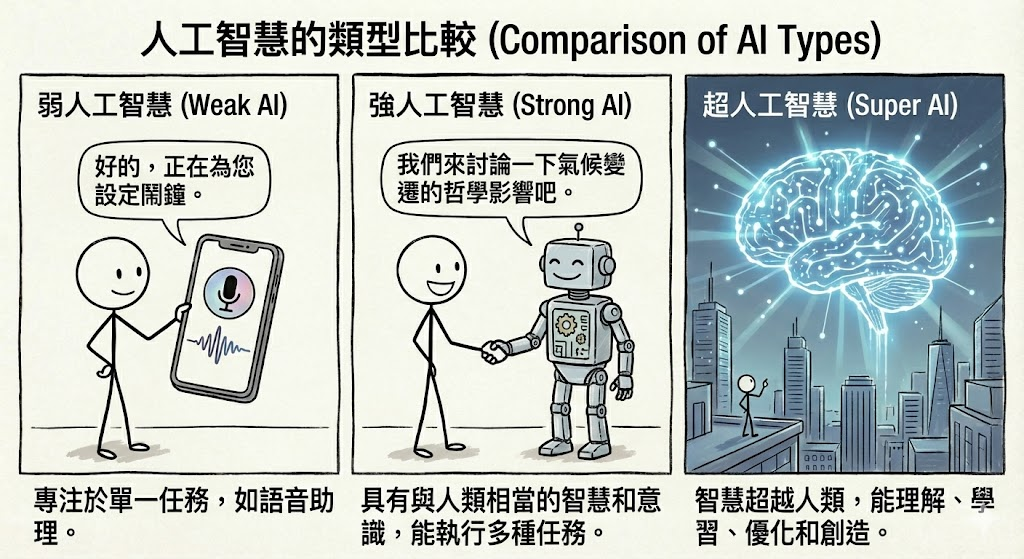
\includegraphics[keepaspectratio]{images/3-ai.jpg}}

}

\caption{AI 的三種型態}

\end{figure}%

\section{符號式 AI (Symbolic AI) 與專家系統}\label{sec-symbolic-ai}

在 AI 發展的早期（1950-1980年代），主流的方法是「符號式 AI」。

\begin{itemize}
\tightlist
\item
  \textbf{核心概念}：認為智慧可以簡化為對符號的邏輯運算。人類將知識編寫成一條條明確的「規則
  (Rules)」，教電腦如何推理。
\item
  \textbf{專家系統 (Expert Systems)} \{\#def-expert-systems\}：是符號式
  AI 的代表。它將人類專家的知識轉化為
  \texttt{If-Then}（如果-那麼）的規則庫。

  \begin{itemize}
  \tightlist
  \item
    \textbf{運作方式}：例如一個醫療診斷系統，規則可能是：「\textbf{如果}病人發燒
    \textbf{且} 咳嗽，\textbf{那麼} 可能是感冒」。
  \item
    \textbf{優點}：邏輯清晰，可解釋性高（我們知道它為什麼這樣判斷）。
  \item
    \textbf{缺點}：

    \begin{itemize}
    \tightlist
    \item
      \textbf{缺乏彈性}：無法處理模糊、不確定或規則難以窮舉的問題（例如：如何定義「貓」的長相？）。一旦遇到規則庫以外的情況，系統就會崩潰。
    \item
      \textbf{知識擷取瓶頸 (Knowledge Acquisition
      Bottleneck)}：將人類專家的隱性知識轉化為明確的規則，需要耗費大量的人力與時間。
    \end{itemize}
  \end{itemize}
\end{itemize}

\section{統計式 AI (Statistical AI)}\label{sec-statistical-ai}

隨著電腦算力的提升和大數據的出現，AI 的發展重心轉向了「統計式
AI」，也就是現在主流的機器學習。

\begin{itemize}
\tightlist
\item
  \textbf{核心概念}：不再由人類手寫規則，而是讓電腦從大量的「數據」中，利用統計學方法自己找出規律和模式。
\item
  \textbf{代表技術}：決策樹 (Decision Tree)、支援向量機
  (SVM)、類神經網路 (Neural Networks) 等。
\item
  \textbf{優勢}：能夠處理複雜、模糊的非結構化數據（如影像、語音、自然語言），並且具備從經驗中學習的能力。
\item
  \textbf{缺點}：

  \begin{itemize}
  \tightlist
  \item
    \textbf{可解釋性低 (Black
    Box)}：統計模型內部的運作複雜，基本上是無法理解的黑盒子，難以解釋為何做出某個判斷。
  \item
    \textbf{依賴數據 (Data
    Dependency)}：模型的好壞取決於數據的品質與數量（Garbage In, Garbage
    Out）。
  \item
    \textbf{偏差風險
    (Bias)}：如果訓練數據包含偏見，模型也會學到這些偏見。
  \end{itemize}
\end{itemize}

\begin{center}\rule{0.5\linewidth}{0.5pt}\end{center}

\chapter{1.2 技術層次關係}\label{ux6280ux8853ux5c64ux6b21ux95dcux4fc2}

要釐清 AI 領域的各種名詞，最簡單的方法是理解它們之間的「包含關係」。

\section{AI、機器學習 (ML)、深度學習 (DL)
的包含關係}\label{sec-ai-ml-dl}

這三者就像是俄羅斯娃娃一樣，一層包著一層：

\begin{enumerate}
\def\labelenumi{\arabic{enumi}.}
\tightlist
\item
  \textbf{人工智慧 (Artificial Intelligence)}
  \{\#def-ai\}：最外層的大圈圈。包含了所有讓機器展現智慧的技術，包括早期的符號式
  AI 和現代的機器學習。
\item
  \textbf{機器學習 (Machine Learning, ML)} \{\#def-ml\}：AI
  的子集。專指那些「不需明確編寫指令，就能讓電腦從數據中學習」的演算法。它包含了傳統的統計學習方法（如決策樹、SVM）和深度學習。
\item
  \textbf{深度學習 (Deep Learning, DL)}
  \{\#def-dl\}：機器學習的子集。特指使用「多層類神經網路 (Deep Neural
  Networks)」來模擬人類大腦運作的技術。它是目前推動 AI 爆發性成長（如
  AlphaGo, ChatGPT）的核心技術。
\end{enumerate}

\begin{figure}[H]

{\centering \pandocbounded{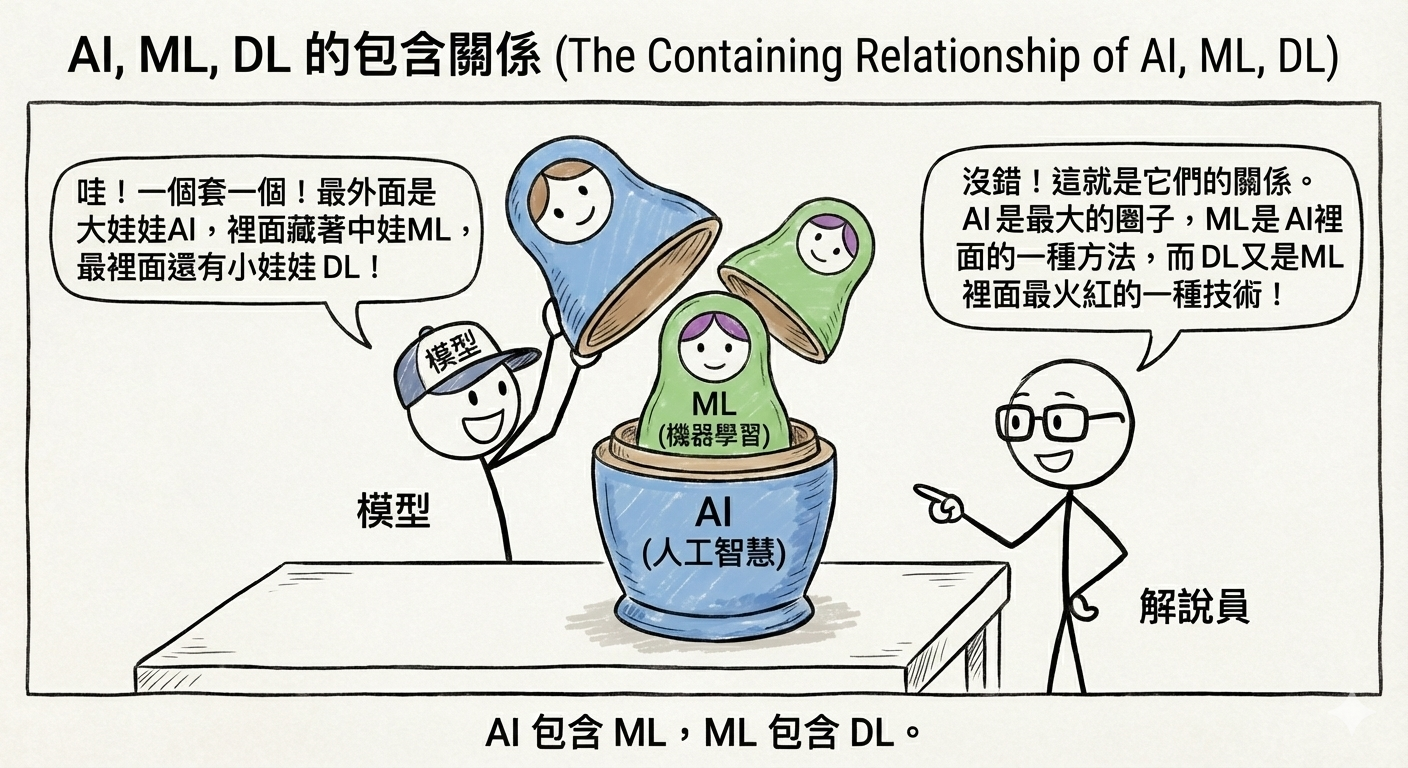
\includegraphics[keepaspectratio]{images/ai-ml-dl.png}}

}

\caption{AI、機器學習、深度學習的包含關係}

\end{figure}%

\section{資料驅動 (Data-Driven) vs.~規則驅動
(Rule-Based)}\label{sec-data-vs-rule}

\begin{itemize}
\tightlist
\item
  \textbf{規則驅動 (Rule-Based)} \{\#def-rule-based\}：

  \begin{itemize}
  \tightlist
  \item
    \textbf{代表}：符號式 AI、專家系統。
  \item
    \textbf{邏輯}：輸入 + 規則 = 輸出。
  \item
    \textbf{比喻}：像是一個只會照著食譜做菜的廚師，食譜沒寫的就不會做。
  \end{itemize}
\item
  \textbf{資料驅動 (Data-Driven)} \{\#def-data-driven\}：

  \begin{itemize}
  \tightlist
  \item
    \textbf{代表}：機器學習、深度學習。
  \item
    \textbf{邏輯}：輸入 + 輸出 = 規則（模型）。
  \item
    \textbf{比喻}：像是一個聰明的學徒，看了一萬次師傅做菜（數據），自己領悟出了做菜的訣竅（模型）。
  \end{itemize}
\end{itemize}

\section{傳統機器學習
vs.~深度學習的適用場景與成本效益分析}\label{sec-ml-vs-dl-cost}

\begin{longtable}[]{@{}
  >{\raggedright\arraybackslash}p{(\linewidth - 4\tabcolsep) * \real{0.3333}}
  >{\raggedright\arraybackslash}p{(\linewidth - 4\tabcolsep) * \real{0.3333}}
  >{\raggedright\arraybackslash}p{(\linewidth - 4\tabcolsep) * \real{0.3333}}@{}}
\toprule\noalign{}
\begin{minipage}[b]{\linewidth}\raggedright
特性
\end{minipage} & \begin{minipage}[b]{\linewidth}\raggedright
傳統機器學習 (Traditional ML)
\end{minipage} & \begin{minipage}[b]{\linewidth}\raggedright
深度學習 (Deep Learning)
\end{minipage} \\
\midrule\noalign{}
\endhead
\bottomrule\noalign{}
\endlastfoot
\textbf{數據需求量} & 較少，小數據集也能運作良好。 &
極大，需要海量數據才能發揮優勢。 \\
\textbf{硬體需求} & 較低，一般 CPU 即可訓練。 & 極高，通常需要高階 GPU
加速運算。 \\
\textbf{特徵工程} &
\textbf{關鍵}。需要人類專家手工提取特徵（如定義貓有尖耳朵）。 &
\textbf{自動化}。模型能自動從數據中提取特徵（End-to-End Learning）。 \\
\textbf{可解釋性} & 較高（如決策樹），容易理解判斷依據。 &
較低（黑盒子），難以解釋神經網路內部的運作。 \\
\textbf{適用場景} & 表格數據 (Tabular Data)、簡單分類、資源受限的環境。
& 影像辨識、自然語言處理 (NLP)、語音生成、複雜決策。 \\
\end{longtable}

\begin{center}\rule{0.5\linewidth}{0.5pt}\end{center}

\chapter{1.3 人類與 AI 的協作模式 (Human-AI
Collaboration)}\label{sec-human-ai-collab}

AI
並非要完全取代人類，更多時候是與人類協作。根據人類介入的程度，我們可以將協作模式分為三種：

\section{1. 人在迴圈中 (Human-in-the-loop, HITL)}\label{sec-hitl}

\begin{itemize}
\tightlist
\item
  \textbf{定義}：人類是 AI 系統運作流程中\textbf{不可或缺}的一部分。AI
  無法獨立完成任務，必須由人類進行確認、修正或提供回饋，系統才能繼續運作或改進。
\item
  \textbf{應用場景}：

  \begin{itemize}
  \tightlist
  \item
    \textbf{資料標註 (Data Labeling)}：AI
    需要人類教它什麼是「貓」。人類負責標記圖片，AI 才能學習。
  \item
    \textbf{醫療診斷輔助}：AI 分析 X
    光片並標記出可疑病灶，但\textbf{最終診斷}必須由醫生確認並簽名。AI
    只是醫生的助手，決策權在人。
  \item
    \textbf{AI 輔助寫作/翻譯}：AI 產生初稿，人類進行潤飾與確認。
  \item
    \textbf{法律合約審查}：AI 標記潛在風險條款，律師進行最終判斷。
  \end{itemize}
\end{itemize}

\section{2. 人在迴圈上 / 人監督迴路 (Human-over-the-loop /
Human-on-the-loop, HOTL)}\label{sec-hotl}

\begin{itemize}
\tightlist
\item
  \textbf{定義}：AI 可以獨立完成大部分的任務，人類扮演\textbf{監督者
  (Supervisor)}
  的角色。人類不直接參與每一個決策，但會監控系統運作，並在發生異常或信心不足時介入。
\item
  \textbf{應用場景}：

  \begin{itemize}
  \tightlist
  \item
    \textbf{智慧工廠監控}：AI
    自動控制生產線的溫度與速度。人類工程師在控制室監控儀表板，只有在警報響起或數值異常時，才手動接管控制。
  \item
    \textbf{自駕車 (Level
    3)}：車輛在高速公路上自動駕駛，但駕駛人必須隨時準備好在系統請求時接手方向盤。
  \item
    \textbf{IT 維運監控 (AIOps)}：AI
    自動偵測並修復常見故障，遇到未知問題才通知工程師。
  \item
    \textbf{智慧交通號誌控制}：AI
    根據車流自動調整紅綠燈，交警僅在特殊狀況（如事故）時介入。
  \end{itemize}
\end{itemize}

\section{3. 人在迴圈外 (Human-out-of-the-loop, HOOTL)}\label{sec-hootl}

\begin{itemize}
\tightlist
\item
  \textbf{定義}：AI
  系統完全\textbf{全自動化}運作，人類不介入其決策過程，甚至無法即時干預。這通常用於需要極快反應速度或人類無法處理的場景。
\item
  \textbf{應用場景}：

  \begin{itemize}
  \tightlist
  \item
    \textbf{高頻交易 (High-Frequency Trading)}：AI
    在毫秒等級內分析股市並自動下單。人類根本來不及反應，只能事後檢討演算法。
  \item
    \textbf{全自動化網路防禦}：面對大規模 DDoS 攻擊，AI
    必須即時自動阻擋惡意流量，等待人類批准會造成系統癱瘓。
  \item
    \textbf{個人化推薦系統}：Netflix 或 YouTube
    根據你的觀看紀錄自動推薦影片，人類完全不介入。
  \item
    \textbf{動態定價 (Dynamic Pricing)}：Uber
    或機票網站根據供需自動調整價格。
  \end{itemize}
\item
  \textbf{風險}：由於人類無法即時監控，HOOTL
  系統必須具備極高的可靠性，並內建嚴格的安全機制 (Safety Guardrails)
  以防止災難性的錯誤（如股市閃崩）。
\end{itemize}

\begin{figure}[H]

{\centering \pandocbounded{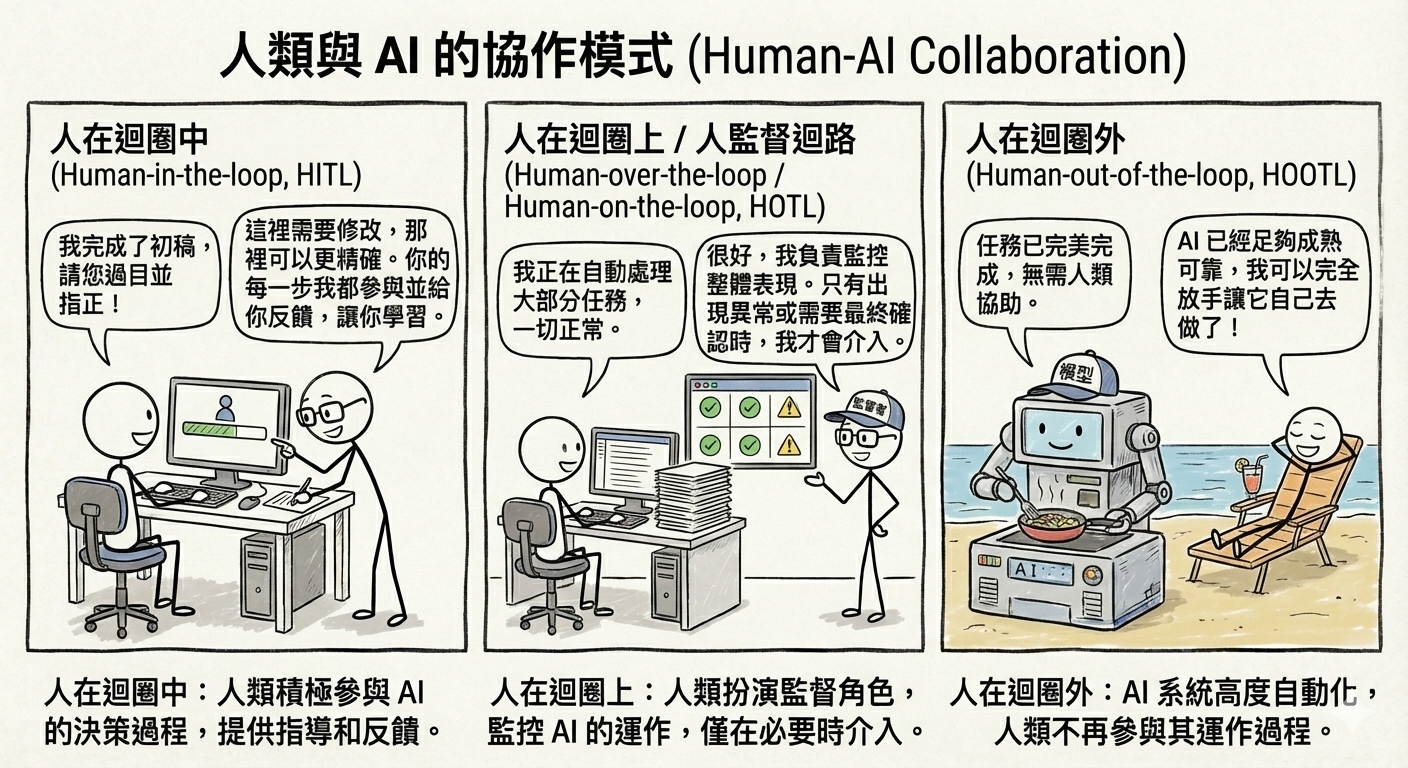
\includegraphics[keepaspectratio]{images/human-ai-collaboration.png}}

}

\caption{Human-AI Collaboration Models}

\end{figure}%

\part{AI 應用問題類型}\label{ai-ux61c9ux7528ux554fux984cux985eux578b}

在開始深入各種技術細節之前，我們需要先了解 AI
究竟能解決什麼樣的問題。這就像在學習使用工具箱之前，先了解有哪些類型的釘子和螺絲一樣。本章將介紹
AI
的學習範式（它是如何學習的）以及資料分析的層次（它能提供多深的見解）。

\chapter{2.1 學習範式}\label{sec-learning-paradigms}

機器學習的核心在於「從資料中學習」。根據資料的型態以及學習的方式，我們可以將其分為幾種主要的範式。

\section{監督式學習 (Supervised
Learning)}\label{sec-supervised-learning}

這是目前應用最廣泛的 AI
學習方式。想像一位\textbf{老師}在教導學生，老師會提供題目（輸入資料）以及標準答案（標籤）。學生的目標是找出題目與答案之間的關聯規則，以便將來遇到沒有答案的新題目時，也能答對。

\begin{itemize}
\tightlist
\item
  \textbf{關鍵要素}：需要有標籤的資料 (Labeled Data)。
\item
  \textbf{生活案例}：

  \begin{itemize}
  \tightlist
  \item
    \textbf{垃圾郵件過濾}：系統看過成千上萬封標示為「垃圾信」或「正常信」的郵件後，學會分辨新郵件。
  \item
    \textbf{房價預測}：根據過去房屋的坪數、地點、屋齡（輸入）以及最終成交價（答案），預測新房子的價格。
  \end{itemize}
\end{itemize}

\section{非監督式學習 (Unsupervised
Learning)}\label{sec-unsupervised-learning}

這種方式就像是\textbf{自修}，或者是一個嬰兒在探索世界。沒有老師告訴它什麼是對的、什麼是錯的，也沒有標準答案。模型必須自己從資料中尋找隱藏的結構或規律。

\begin{itemize}
\tightlist
\item
  \textbf{關鍵要素}：只有輸入資料，沒有標籤。
\item
  \textbf{生活案例}：

  \begin{itemize}
  \tightlist
  \item
    \textbf{顧客分群 (Customer
    Segmentation)}：電商平台分析消費者的購買紀錄，自動將顧客分成「精打細算型」、「衝動購物型」等群體，但系統事先並不知道這些群體的定義。
  \item
    \textbf{異常偵測}：信用卡公司分析刷卡行為，發現某筆交易與平常的模式差異過大，判定為潛在盜刷。
  \end{itemize}
\end{itemize}

\begin{figure}[H]

{\centering \pandocbounded{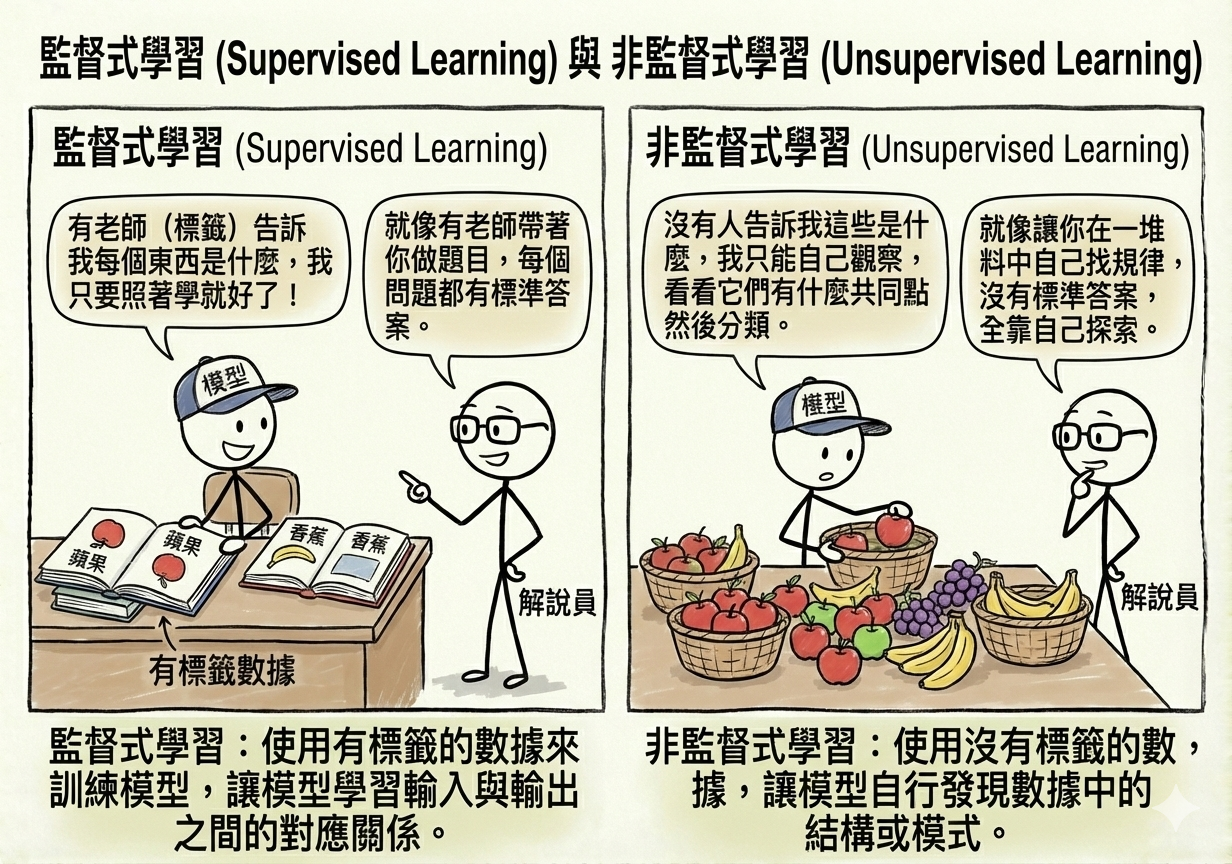
\includegraphics[keepaspectratio]{images/supervised.png}}

}

\caption{監督式學習與非監督式學習}

\end{figure}%

\section{半監督式學習 (Semi-supervised
Learning)}\label{sec-semi-supervised-learning}

這是一種折衷方案。在現實世界中，取得有標籤的資料往往很昂貴（需要人工標註），但沒標籤的資料卻隨處可見。半監督式學習結合了少量的標籤資料和大量的無標籤資料。

\begin{itemize}
\tightlist
\item
  \textbf{類比}：老師只教了幾個核心概念（少量標籤），剩下的要學生舉一反三，從大量練習題中自己摸索（大量無標籤）。
\item
  \textbf{應用}：醫療影像分析（醫生標註幾張 X
  光片很花時間，但醫院有大量未標註的片子）。
\end{itemize}

\begin{figure}[H]

{\centering \pandocbounded{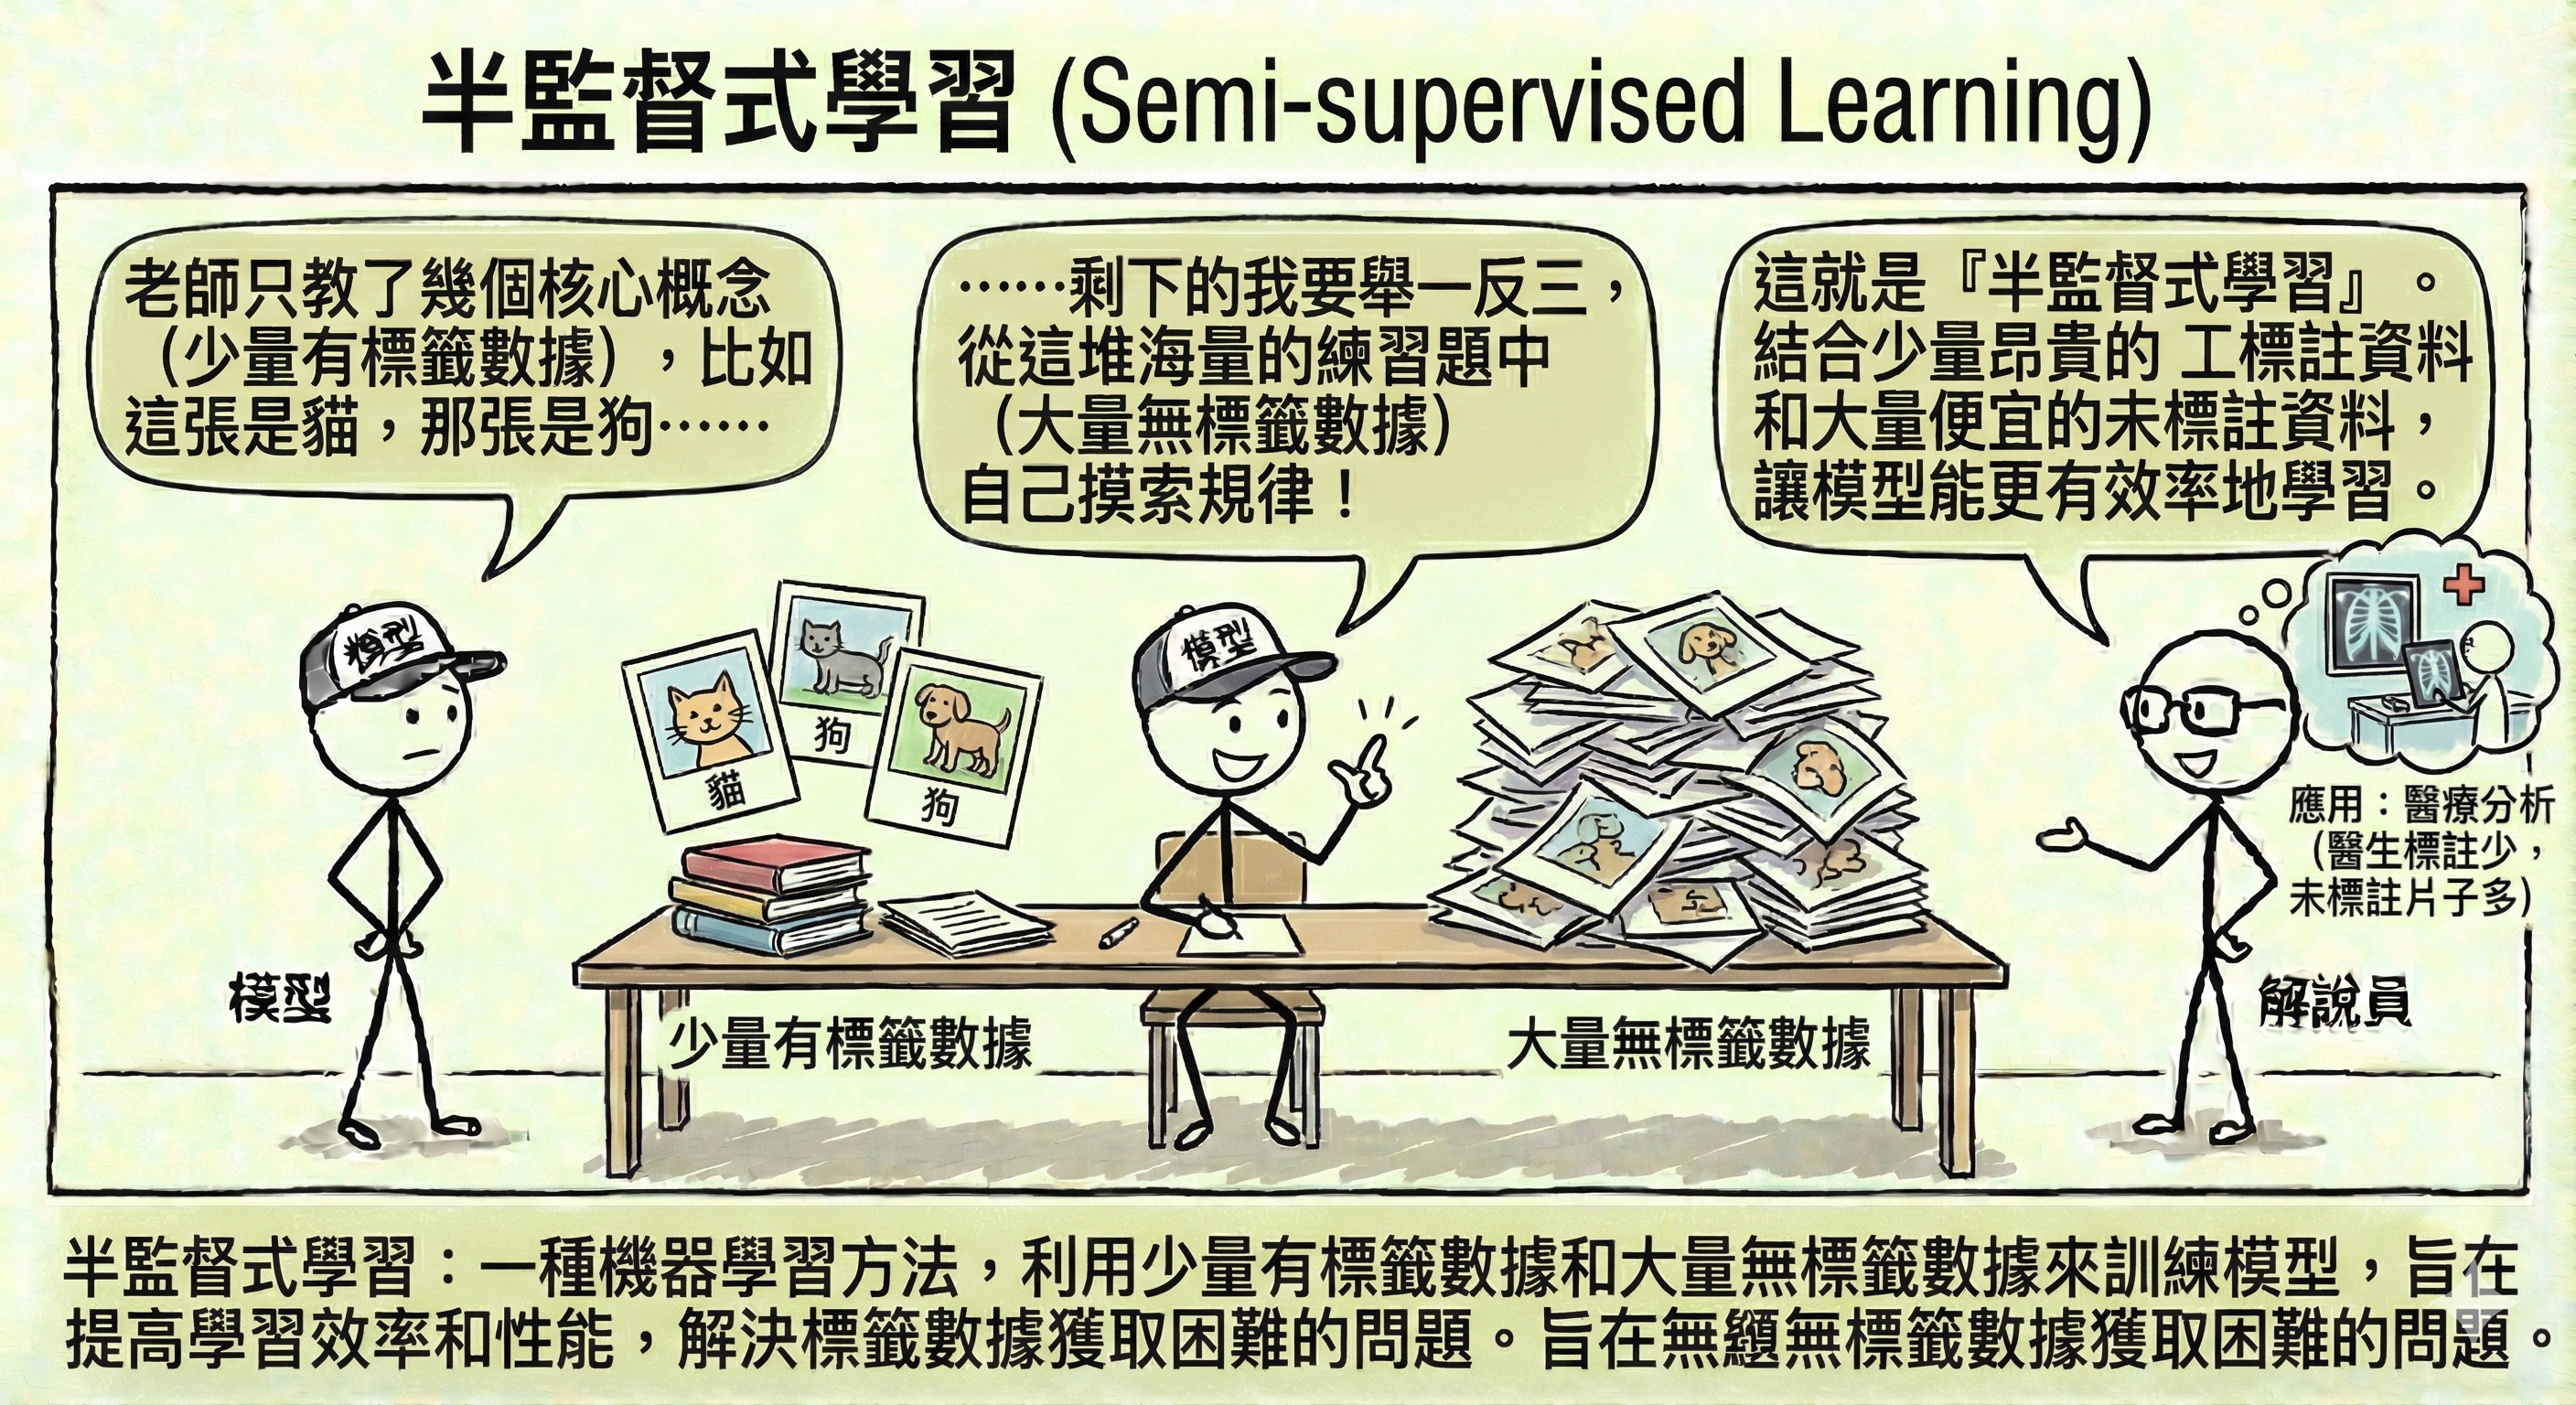
\includegraphics[keepaspectratio]{images/semi-supervised.png}}

}

\caption{半監督式學習}

\end{figure}%

\section{強化學習 (Reinforcement
Learning)}\label{sec-reinforcement-learning}

這就像是\textbf{訓練寵物}。我們不會直接告訴 AI
每一步該怎麼走，而是讓它在一個環境中嘗試。做對了就給予獎勵（Reward），做錯了就給予懲罰（Penalty）。AI
的目標是透過不斷嘗試錯誤（Trial and
Error），找出能獲得最大累積獎勵的策略。

強化學習的過程可以拆解為以下幾個關鍵要素的互動：

\begin{enumerate}
\def\labelenumi{\arabic{enumi}.}
\tightlist
\item
  \textbf{代理人 (Agent)}：也就是正在學習的 AI
  模型（例如：掃地機器人）。
\item
  \textbf{環境
  (Environment)}：代理人所處的世界（例如：充滿家具的客廳）。
\item
  \textbf{狀態 (State)}：代理人當前的情況（例如：前方 10
  公分有障礙物）。
\item
  \textbf{行動 (Action)}：代理人採取的動作（例如：向左轉）。
\item
  \textbf{獎勵 (Reward)}：環境給予的回饋（例如：成功避開障礙物得 +1
  分，撞到桌腳得 -10 分）。
\end{enumerate}

\textbf{探索與利用 (Exploration vs.~Exploitation)}

強化學習中有一個經典的難題： * \textbf{探索
(Exploration)}：嘗試新的、未知的行動，希望能發現更好的策略（但也可能失敗）。
* \textbf{利用
(Exploitation)}：堅持目前已知最好的策略，確保獲得穩定的獎勵。 AI
必須在這兩者之間取得平衡，才能不斷進步。

\begin{itemize}
\tightlist
\item
  \textbf{生活案例}：

  \begin{itemize}
  \tightlist
  \item
    \textbf{AlphaGo}：圍棋程式透過無數次的自我對弈，學習如何贏得比賽。它不僅學習人類棋譜，更透過自我探索發現了人類未曾想過的下法。
  \item
    \textbf{掃地機器人}：在房間裡碰撞學習，慢慢規劃出最有效率的清掃路徑，同時避開障礙物。
  \end{itemize}
\end{itemize}

\begin{figure}[H]

{\centering \pandocbounded{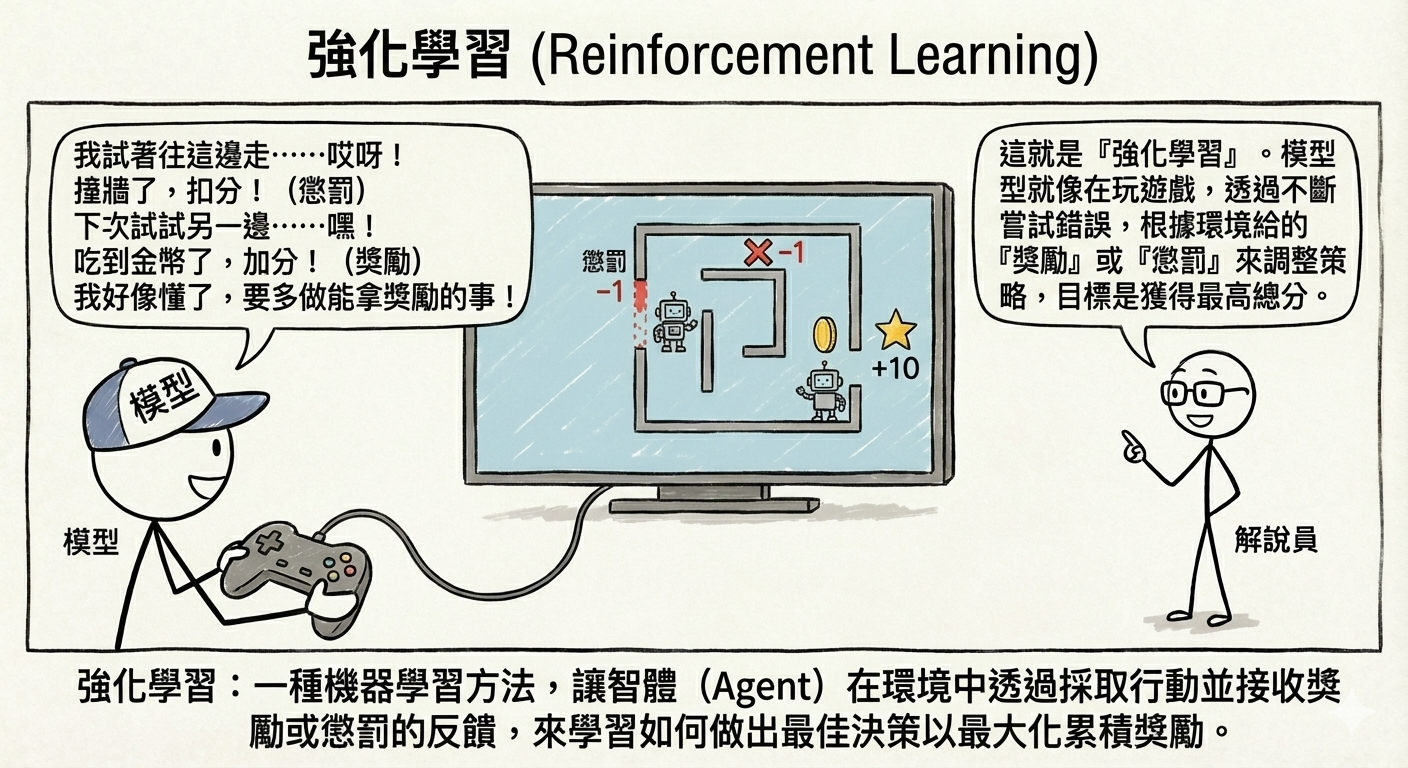
\includegraphics[keepaspectratio]{images/reinforcement-learning.png}}

}

\caption{強化學習}

\end{figure}%

\section{遷移學習 (Transfer Learning)}\label{sec-transfer-learning}

這就是所謂的「站在巨人的肩膀上」。人類在學習新技能時，通常會運用舊有的經驗。例如學會騎腳踏車的人，學騎機車會比較快。遷移學習就是將一個已經訓練好的強大模型（預訓練模型），微調後應用到新的、類似的任務上。

\begin{itemize}
\tightlist
\item
  \textbf{優勢}：不需要從頭開始訓練，大幅節省時間與資料需求。
\item
  \textbf{生活案例}：

  \begin{itemize}
  \tightlist
  \item
    \textbf{醫療影像診斷}：使用一個已經看過數百萬張日常照片（如貓、狗、車）的模型，因為它已經學會了如何辨識邊緣、形狀和紋理，只需要再給它少量的
    X 光片或 MRI 影像，它就能快速學會判讀病灶。
  \item
    \textbf{特定領域的語言模型}：使用像 GPT
    這樣已經讀過整個網際網路的通用模型，針對「法律文件」或「醫療報告」進行微調，讓它變成該領域的專家助手。
  \item
    \textbf{風格轉換}：將一位畫家（如梵谷）的畫風「遷移」到一張普通的風景照上，讓照片瞬間變成名畫風格。
  \end{itemize}
\end{itemize}

\begin{figure}[H]

{\centering \pandocbounded{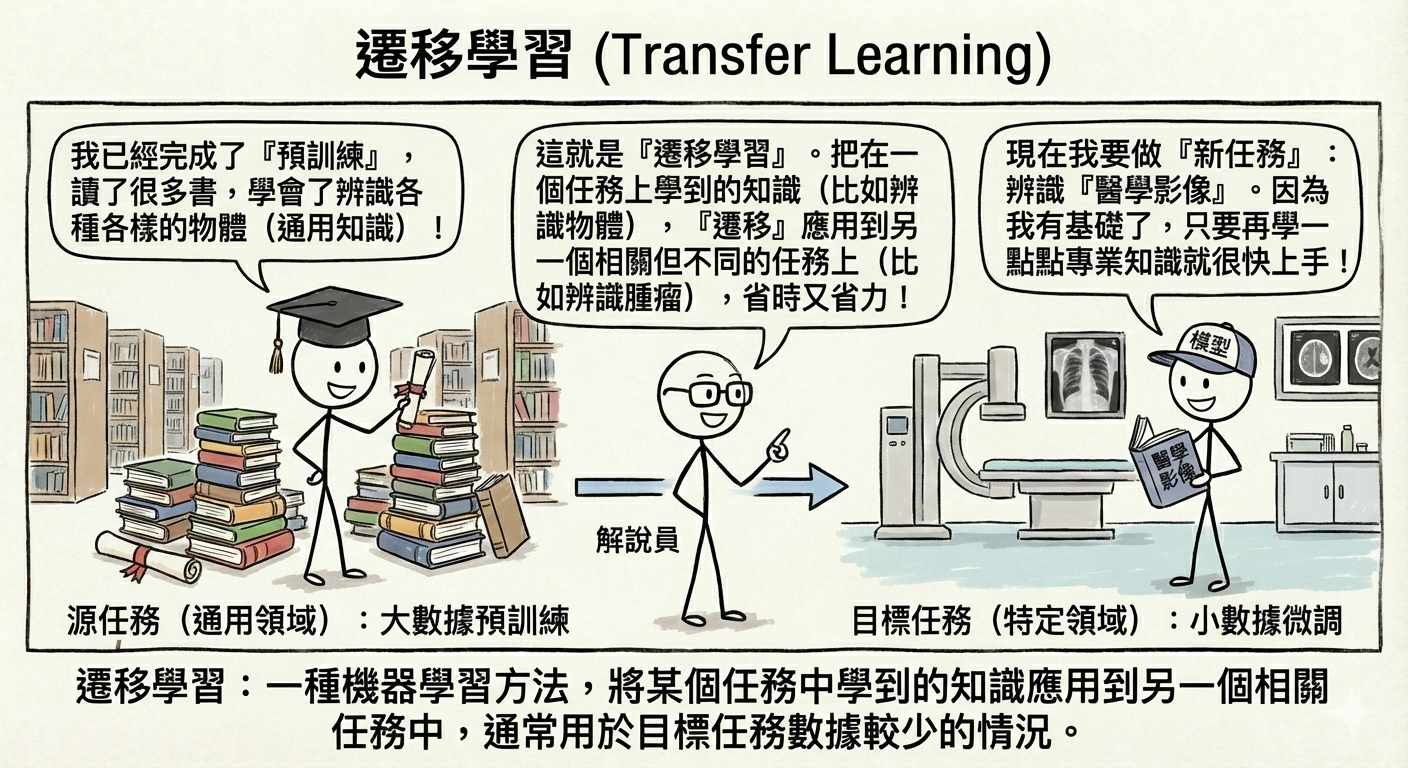
\includegraphics[keepaspectratio]{images/transfer-learning.png}}

}

\caption{遷移學習}

\end{figure}%

\chapter{2.2 資料分析層次}\label{sec-data-analysis-levels}

AI
與資料科學不僅僅是預測未來，它在商業應用上通常被分為四個價值層次，由淺入深：

\section{1. 描述性分析 (Descriptive Analysis):
發生了什麼？}\label{sec-descriptive-analysis}

這是最基礎的層次，重點在於\textbf{總結過去}。透過報表、儀表板
(Dashboard) 來呈現歷史數據。 * \textbf{例子}： *
\textbf{銷售報表}：上個月的總銷售額是多少？哪個產品賣得最好？ *
\textbf{網站分析}：昨天有多少人造訪網站？平均停留時間多久？ *
\textbf{人資盤點}：目前公司有多少員工？各部門的人數分佈為何？

\begin{figure}[H]

{\centering \pandocbounded{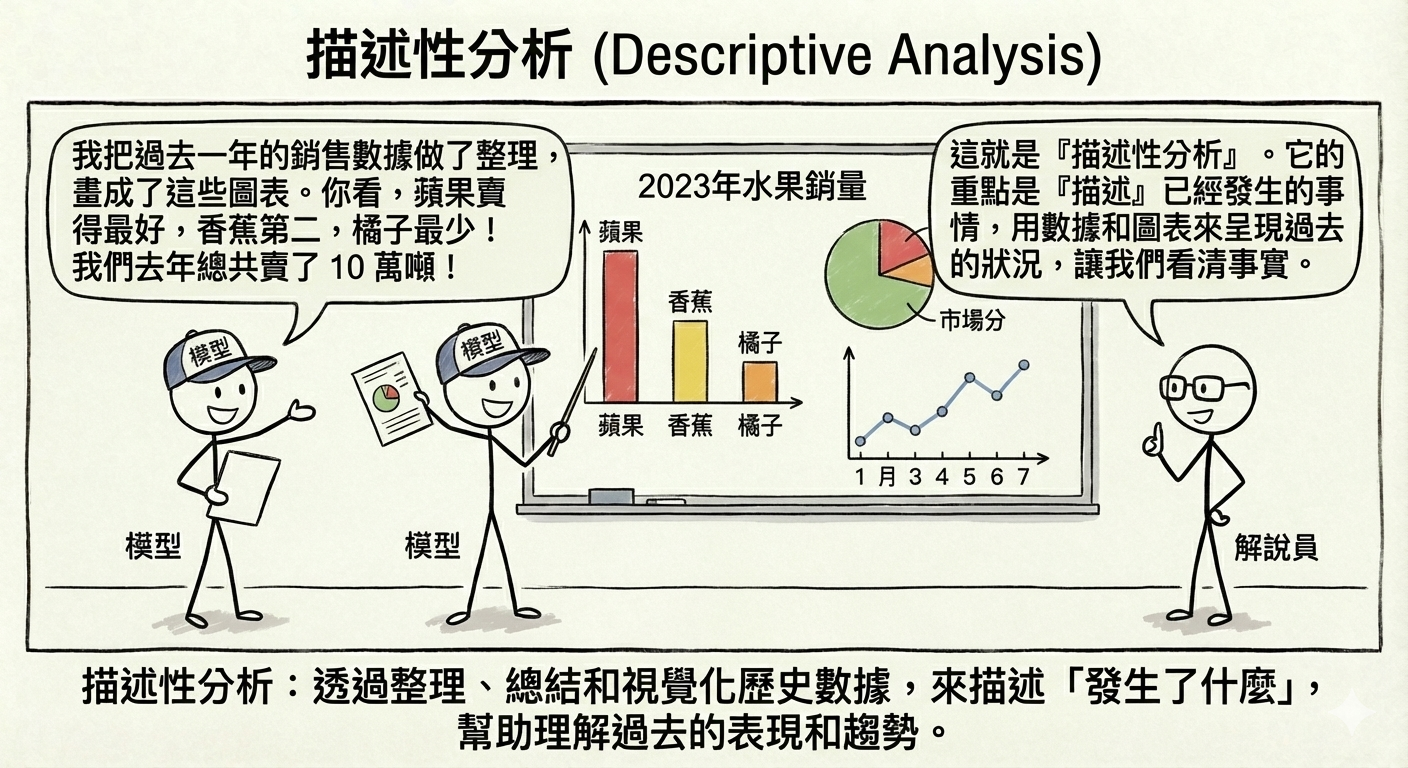
\includegraphics[keepaspectratio]{images/descriptive-analysis.png}}

}

\caption{描述性分析}

\end{figure}%

\section{2. 診斷性分析 (Diagnostic Analysis):
為什麼發生？}\label{sec-diagnostic-analysis}

這層次試圖找出\textbf{原因}。透過資料鑽取 (Drill-down)
或相關性分析，解釋過去事件的成因。 * \textbf{例子}： *
\textbf{銷售檢討}：為什麼上個月銷售額下降？是因為季節性因素，還是競爭對手降價？
* \textbf{設備故障}：為什麼這台機器突然停機？是因為過熱還是零件磨損？ *
\textbf{客戶流失}：為什麼這群客戶不再續約？是因為價格太高還是服務滿意度下降？

\begin{figure}[H]

{\centering \pandocbounded{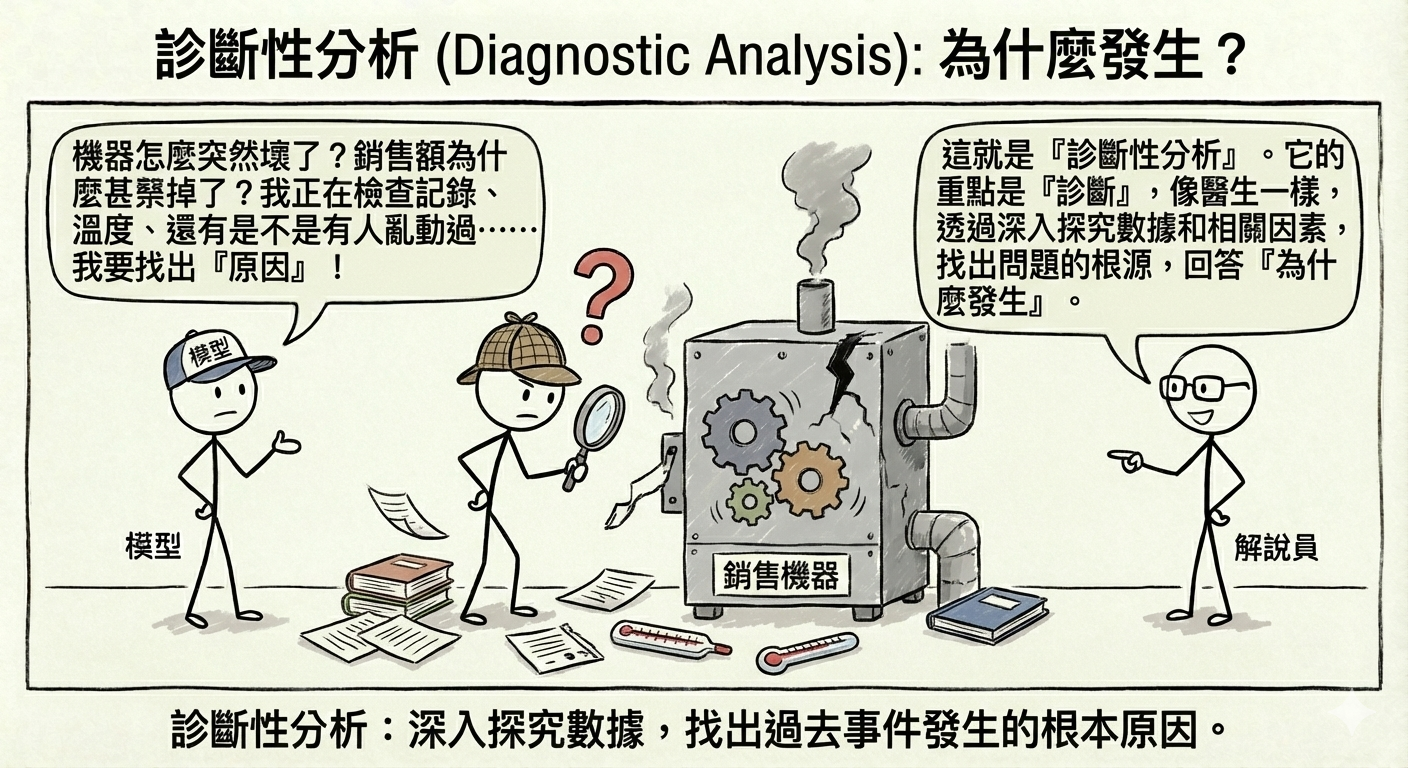
\includegraphics[keepaspectratio]{images/diagnostic-analysis.png}}

}

\caption{診斷性分析}

\end{figure}%

\section{3. 預測性分析 (Predictive Analysis):
將會發生什麼？}\label{sec-predictive-analysis}

這正是 AI
與機器學習大顯身手的地方。利用過去的模式來\textbf{預測未來}的趨勢或事件。
* \textbf{例子}： *
\textbf{銷售預測}：根據目前的趨勢，下個月的銷售額預計會是多少？ *
\textbf{預防性維護}：這台機器在未來一週內故障的機率有多高？ *
\textbf{信用評分}：這位申請人未來違約的機率是多少？

\begin{figure}[H]

{\centering \pandocbounded{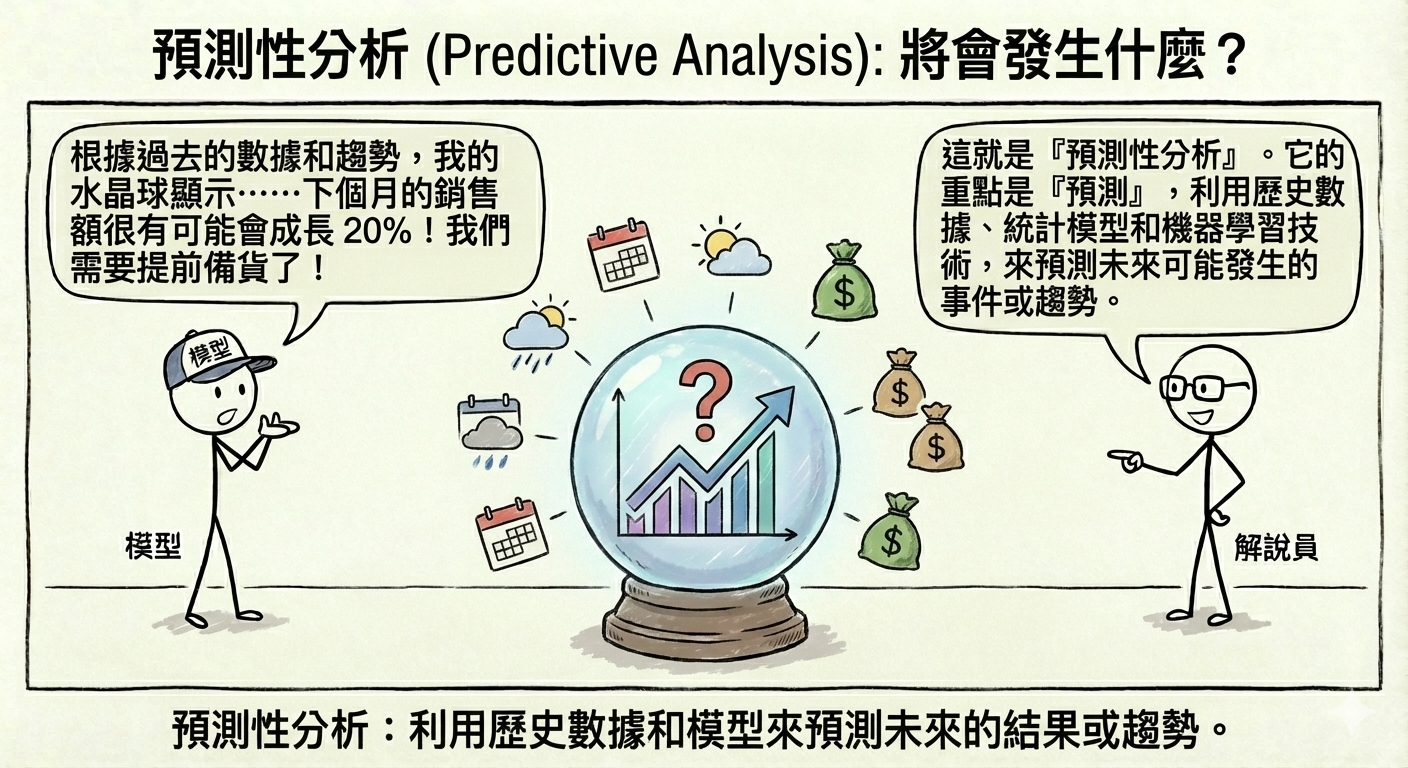
\includegraphics[keepaspectratio]{images/predictive-analysis.png}}

}

\caption{預測性分析}

\end{figure}%

\section{4. 處方性分析 (Prescriptive Analysis):
應該怎麼做？}\label{sec-prescriptive-analysis}

這是分析的最高境界。不僅預測未來，還能提供\textbf{最佳行動建議}，告訴決策者如何優化結果。
* \textbf{例子}： *
\textbf{庫存優化}：既然預測下個月庫存會不足，系統建議現在應該向供應商 A
訂購 500 個零件，並向供應商 B 訂購 300 個，以達到成本最低且到貨最快。 *
\textbf{路徑規劃}：考量到預測的塞車狀況，導航系統建議司機改走 B
路線以節省 10 分鐘。 * \textbf{行銷配置}：為了最大化轉換率，系統建議將
60\% 的預算投入 Instagram 廣告，40\% 投入 Google 關鍵字。

\begin{figure}[H]

{\centering \pandocbounded{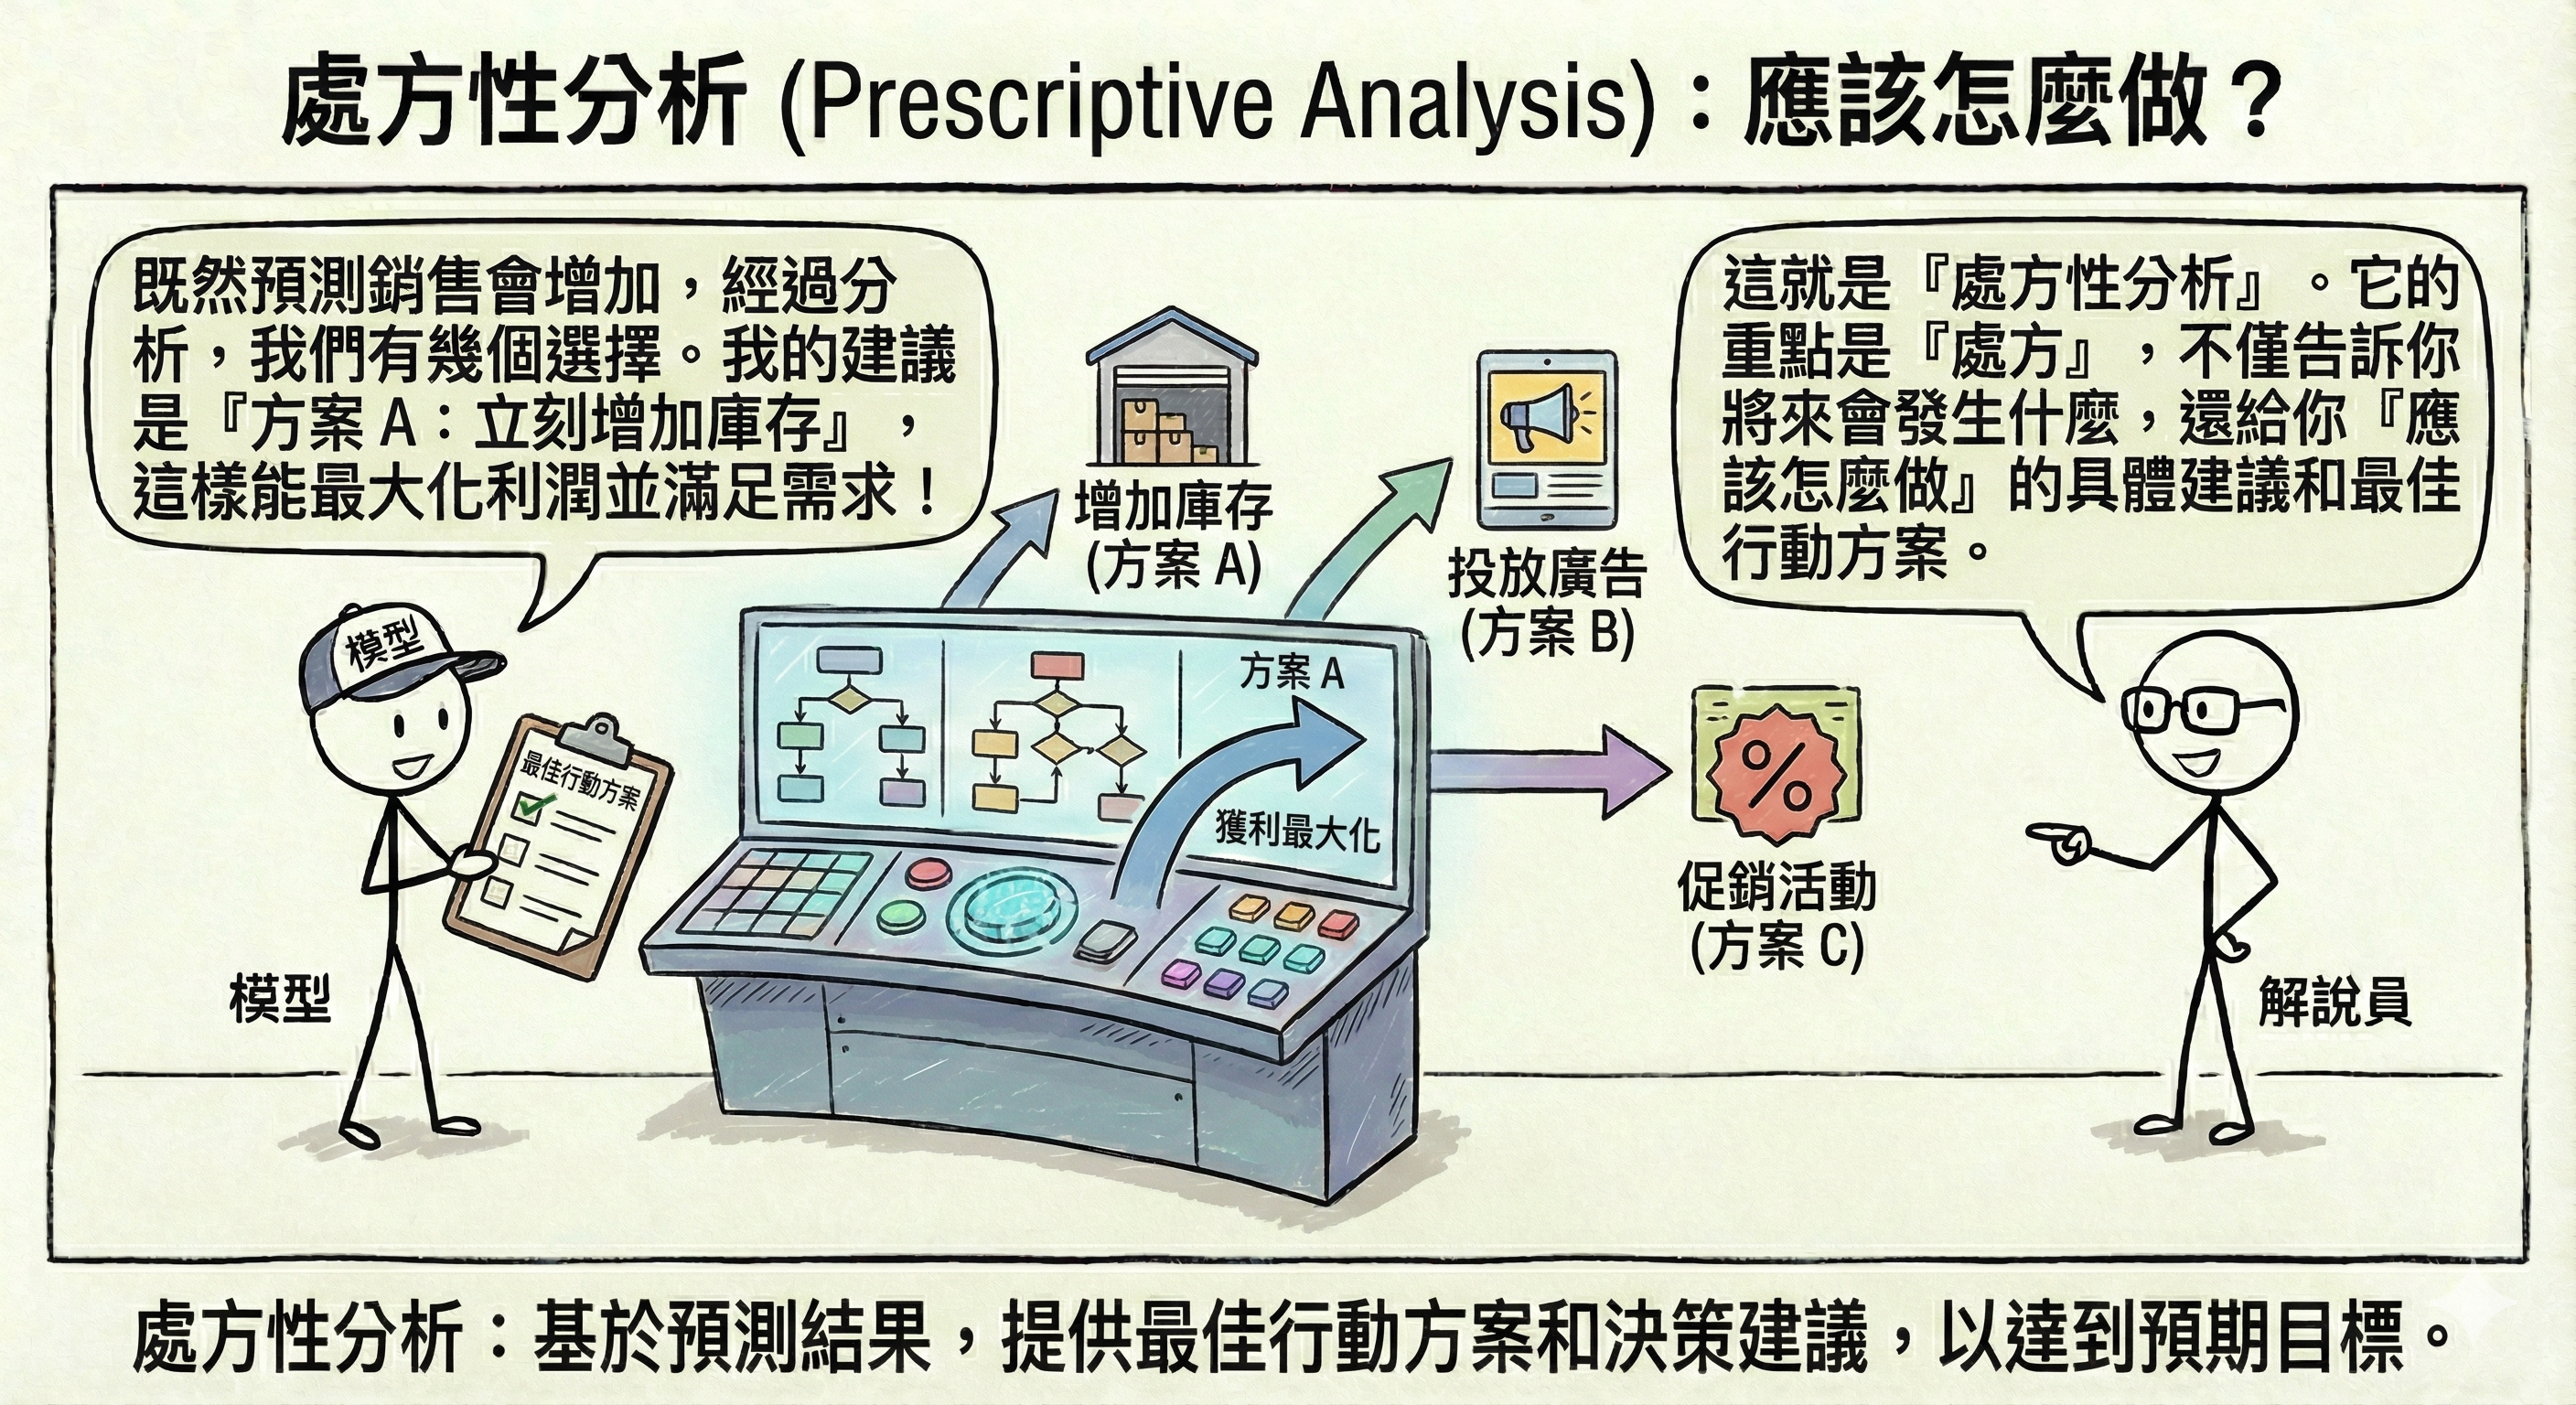
\includegraphics[keepaspectratio]{images/prescriptive-analysis.png}}

}

\caption{處方性分析}

\end{figure}%

\chapter{本章總結與考點提示}\label{sec-chapter2-summary}

\section{核心概念回顧}\label{ux6838ux5fc3ux6982ux5ff5ux56deux9867}

本章介紹了 AI 應用的兩大基礎框架：\textbf{學習範式}（AI
如何學習）與\textbf{資料分析層次}（AI 能提供什麼價值）。

\textbf{學習範式比較表}：

\begin{longtable}[]{@{}
  >{\raggedright\arraybackslash}p{(\linewidth - 6\tabcolsep) * \real{0.2500}}
  >{\raggedright\arraybackslash}p{(\linewidth - 6\tabcolsep) * \real{0.2500}}
  >{\raggedright\arraybackslash}p{(\linewidth - 6\tabcolsep) * \real{0.2500}}
  >{\raggedright\arraybackslash}p{(\linewidth - 6\tabcolsep) * \real{0.2500}}@{}}
\toprule\noalign{}
\begin{minipage}[b]{\linewidth}\raggedright
學習範式
\end{minipage} & \begin{minipage}[b]{\linewidth}\raggedright
資料特性
\end{minipage} & \begin{minipage}[b]{\linewidth}\raggedright
典型應用
\end{minipage} & \begin{minipage}[b]{\linewidth}\raggedright
關鍵概念
\end{minipage} \\
\midrule\noalign{}
\endhead
\bottomrule\noalign{}
\endlastfoot
\textbf{監督式學習} & 有標籤資料 & 分類、迴歸 & 訓練集、測試集 \\
\textbf{非監督式學習} & 無標籤資料 & 分群、降維 & 隱藏結構、模式發現 \\
\textbf{半監督式學習} & 少量標籤 + 大量無標籤 & 醫療影像 & 標註成本 \\
\textbf{強化學習} & 獎勵/懲罰訊號 & 遊戲、機器人 &
Agent、Environment、Policy \\
\textbf{遷移學習} & 預訓練模型 & 微調應用 & Pre-training、Fine-tuning \\
\end{longtable}

\textbf{資料分析層次}：

\begin{enumerate}
\def\labelenumi{\arabic{enumi}.}
\tightlist
\item
  \textbf{描述性} → 發生了什麼？（報表、儀表板）
\item
  \textbf{診斷性} → 為什麼發生？（根因分析）
\item
  \textbf{預測性} → 將會發生什麼？（機器學習預測）
\item
  \textbf{處方性} → 應該怎麼做？（最佳化建議）
\end{enumerate}

\section{AI
應用規劃師認證考點}\label{ai-ux61c9ux7528ux898fux5283ux5e2bux8a8dux8b49ux8003ux9ede}

\textbf{常考題型與解題策略}：

\begin{enumerate}
\def\labelenumi{\arabic{enumi}.}
\tightlist
\item
  \textbf{情境判斷題}：給定商業問題，選擇最適合的學習範式

  \begin{itemize}
  \tightlist
  \item
    \emph{例題}：「公司想根據客戶過去的購買紀錄預測流失率」

    \begin{itemize}
    \tightlist
    \item
      \textbf{解答}：監督式學習（分類問題）
    \item
      \textbf{關鍵字}：「過去紀錄」= 有標籤資料；「預測」= 監督式學習
    \end{itemize}
  \item
    \emph{例題}：「想將客戶分成不同群組進行精準行銷，但不知道該分幾群」

    \begin{itemize}
    \tightlist
    \item
      \textbf{解答}：非監督式學習（分群）
    \item
      \textbf{關鍵字}：「不知道分幾群」= 無預設標籤；「分群」=
      非監督式學習
    \end{itemize}
  \end{itemize}
\item
  \textbf{分析層次判斷題}：識別問題屬於哪個分析層次

  \begin{itemize}
  \tightlist
  \item
    \emph{例題}：「為什麼上個月銷售下降？」→
    \textbf{診斷性分析}（找原因）
  \item
    \emph{例題}：「下個月銷售會是多少？」→
    \textbf{預測性分析}（預測未來）
  \item
    \emph{例題}：「應該如何調整行銷策略以提升銷售？」→
    \textbf{處方性分析}（給建議）
  \end{itemize}
\item
  \textbf{概念辨析題}：

  \begin{itemize}
  \tightlist
  \item
    \textbf{監督 vs.~非監督}：關鍵在於「是否有標籤」
  \item
    \textbf{強化學習的特點}：透過「試錯」學習，需要「獎勵機制」
  \item
    \textbf{遷移學習的優勢}：「站在巨人肩膀上」，減少訓練時間與資料需求
  \item
    \textbf{探索
    vs.~利用}：新嘗試（可能更好但有風險）vs.~已知最佳（穩定但不會進步）
  \end{itemize}
\item
  \textbf{應用場景配對題}：

  \begin{itemize}
  \tightlist
  \item
    垃圾郵件過濾 → 監督式學習（分類）
  \item
    客戶分群 → 非監督式學習
  \item
    AlphaGo 圍棋 → 強化學習
  \item
    醫療影像診斷（資料少）→ 遷移學習
  \item
    異常交易偵測 → 非監督式學習（異常偵測）
  \end{itemize}
\end{enumerate}

\section{記憶口訣}\label{ux8a18ux61b6ux53e3ux8a23}

\begin{itemize}
\tightlist
\item
  \textbf{學習範式}：「監非半強遷」（監督、非監督、半監督、強化、遷移）
\item
  \textbf{分析層次}：「描診預處」（描述、診斷、預測、處方）
\item
  \textbf{強化學習}：「代環狀動獎」（代理人、環境、狀態、行動、獎勵）
\end{itemize}

\section{延伸思考}\label{ux5ef6ux4f38ux601dux8003}

\begin{itemize}
\tightlist
\item
  為什麼 AlphaGo 使用強化學習而不是監督式學習？
\item
  在什麼情況下，描述性分析就足夠了，不需要預測性分析？
\item
  遷移學習為何能讓小公司也能使用 AI？
\end{itemize}

\part{第二部：數據工程------AI 的堅實地基}

\part{數據處理生命週期與架構}\label{ux6578ux64daux8655ux7406ux751fux547dux9031ux671fux8207ux67b6ux69cb}

在 AI 的世界裡，有一句名言：「垃圾進，垃圾出 (Garbage In, Garbage Out,
GIGO)」。無論你的模型多麼先進，如果餵給它的資料品質低劣，結果也將毫無價值。本章將探討資料如何從原始狀態，經過層層處理，最終變成模型可用的燃料。

\chapter{3.1 資料管道 (Data Pipeline)}\label{sec-data-pipeline}

資料管道就像是城市的\textbf{供水系統}。水源（原始資料）可能來自水庫、河流或地下水，必須經過過濾、消毒、輸送（處理過程），最後才能從家裡的水龍頭流出乾淨的自來水（可用資料）。

\section{ETL (Extract-Transform-Load) 架構}\label{sec-etl}

這是最傳統也最常見的資料處理流程，特別適用於結構化資料（如資料庫表格）。

\begin{enumerate}
\def\labelenumi{\arabic{enumi}.}
\tightlist
\item
  \textbf{資料擷取
  (Extract)}：從各種來源（資料庫、API、檔案）收集資料。就像去市場\textbf{買菜}。
\item
  \textbf{資料轉換
  (Transform)}：清洗、格式化、計算衍生欄位。就像在廚房\textbf{備料}（洗菜、切肉、醃製）。這是最耗時的步驟。
\item
  \textbf{資料載入 (Load)}：將處理好的資料存入目標系統（通常是資料倉儲
  Data Warehouse）。就像將煮好的菜\textbf{端上桌}。
\end{enumerate}

\begin{itemize}
\tightlist
\item
  \textbf{特點}：先處理再儲存，確保進入倉庫的資料都是乾淨、格式統一的。但若需求變更，需要重新設計轉換流程。
\end{itemize}

\section{ELT (Extract-Load-Transform) 架構與資料湖 (Data
Lake)}\label{sec-elt}

隨著大數據 (Big Data)
的興起，資料量大到無法先處理再儲存，或者資料是非結構化的（如日誌、圖片、影片），ELT
架構應運而生。

\begin{itemize}
\tightlist
\item
  \textbf{流程}：先把所有資料（不管髒不髒）全部抓進來（Extract \&
  Load），存放在一個巨大的儲存庫中，稱為\textbf{資料湖 (Data
  Lake)}。等到需要分析時，再進行轉換 (Transform)。
\item
  \textbf{類比}：這就像\textbf{搬家}。先把舊家的東西全部裝箱搬到新家（Load），等到要用某個東西時，再打開箱子整理（Transform）。
\item
  \textbf{優勢}：靈活、速度快，保留了原始資料的細節。
\end{itemize}

\section{批次處理 vs.~串流處理}\label{sec-batch-vs-streaming}

\begin{itemize}
\tightlist
\item
  \textbf{批次處理 (Batch
  Processing)}：累積一段時間的資料後，一次性處理。

  \begin{itemize}
  \tightlist
  \item
    \textbf{類比}：\textbf{公車}。要等到時刻表到了或人坐滿了才發車。
  \item
    \textbf{適用}：日報表、月結算、不需要即時性的分析。
  \end{itemize}
\item
  \textbf{串流處理 (Streaming Processing)}：資料一產生就立刻處理。

  \begin{itemize}
  \tightlist
  \item
    \textbf{類比}：\textbf{計程車}。隨叫隨走，來一個載一個。
  \item
    \textbf{適用}：即時詐欺偵測、股市交易監控、即時推薦系統。
  \end{itemize}
\end{itemize}

\chapter{3.2 探索性資料分析 (EDA)}\label{sec-eda}

在正式建模之前，我們必須先「認識」資料。探索性資料分析 (Exploratory Data
Analysis, EDA)
就像是\textbf{相親}，你需要透過各種方式了解對方的個性、習慣和背景。

\section{統計摘要 (Descriptive
Statistics)}\label{sec-descriptive-statistics}

用數字來描述資料的整體樣貌。

\begin{itemize}
\tightlist
\item
  \textbf{集中趨勢}：尋找資料的「中心」。

  \begin{itemize}
  \tightlist
  \item
    \textbf{平均數
    (Mean)}：所有數值加總除以個數。容易受極端值影響（如比爾蓋茲走進酒吧，平均財富瞬間飆升）。
  \item
    \textbf{中位數
    (Median)}：將資料由小到大排列，位於中間的那個數。代表「一般人」的水準，不受極端值影響。
  \item
    \textbf{眾數 (Mode)}：出現次數最多的數值。
  \end{itemize}
\item
  \textbf{離散程度}：資料分佈得有多「散」。

  \begin{itemize}
  \tightlist
  \item
    \textbf{標準差 (Standard
    Deviation)}：數值與平均數的平均距離。標準差越大，代表資料越參差不齊。
  \item
    \textbf{四分位數 (Quartiles)}：將資料切成四等份的切點。
  \end{itemize}
\item
  \textbf{偏態 (Skewness)}：資料分佈是偏左還是偏右。
\end{itemize}

\section{資料視覺化決策邏輯}\label{sec-data-visualization}

一張圖勝過千言萬語，但選錯圖表會造成誤導。

\begin{itemize}
\item
  \textbf{散佈圖 (Scatter
  Plot)}：看兩個變數之間的\textbf{關聯}（例如：身高 vs.~體重）。
  \pandocbounded{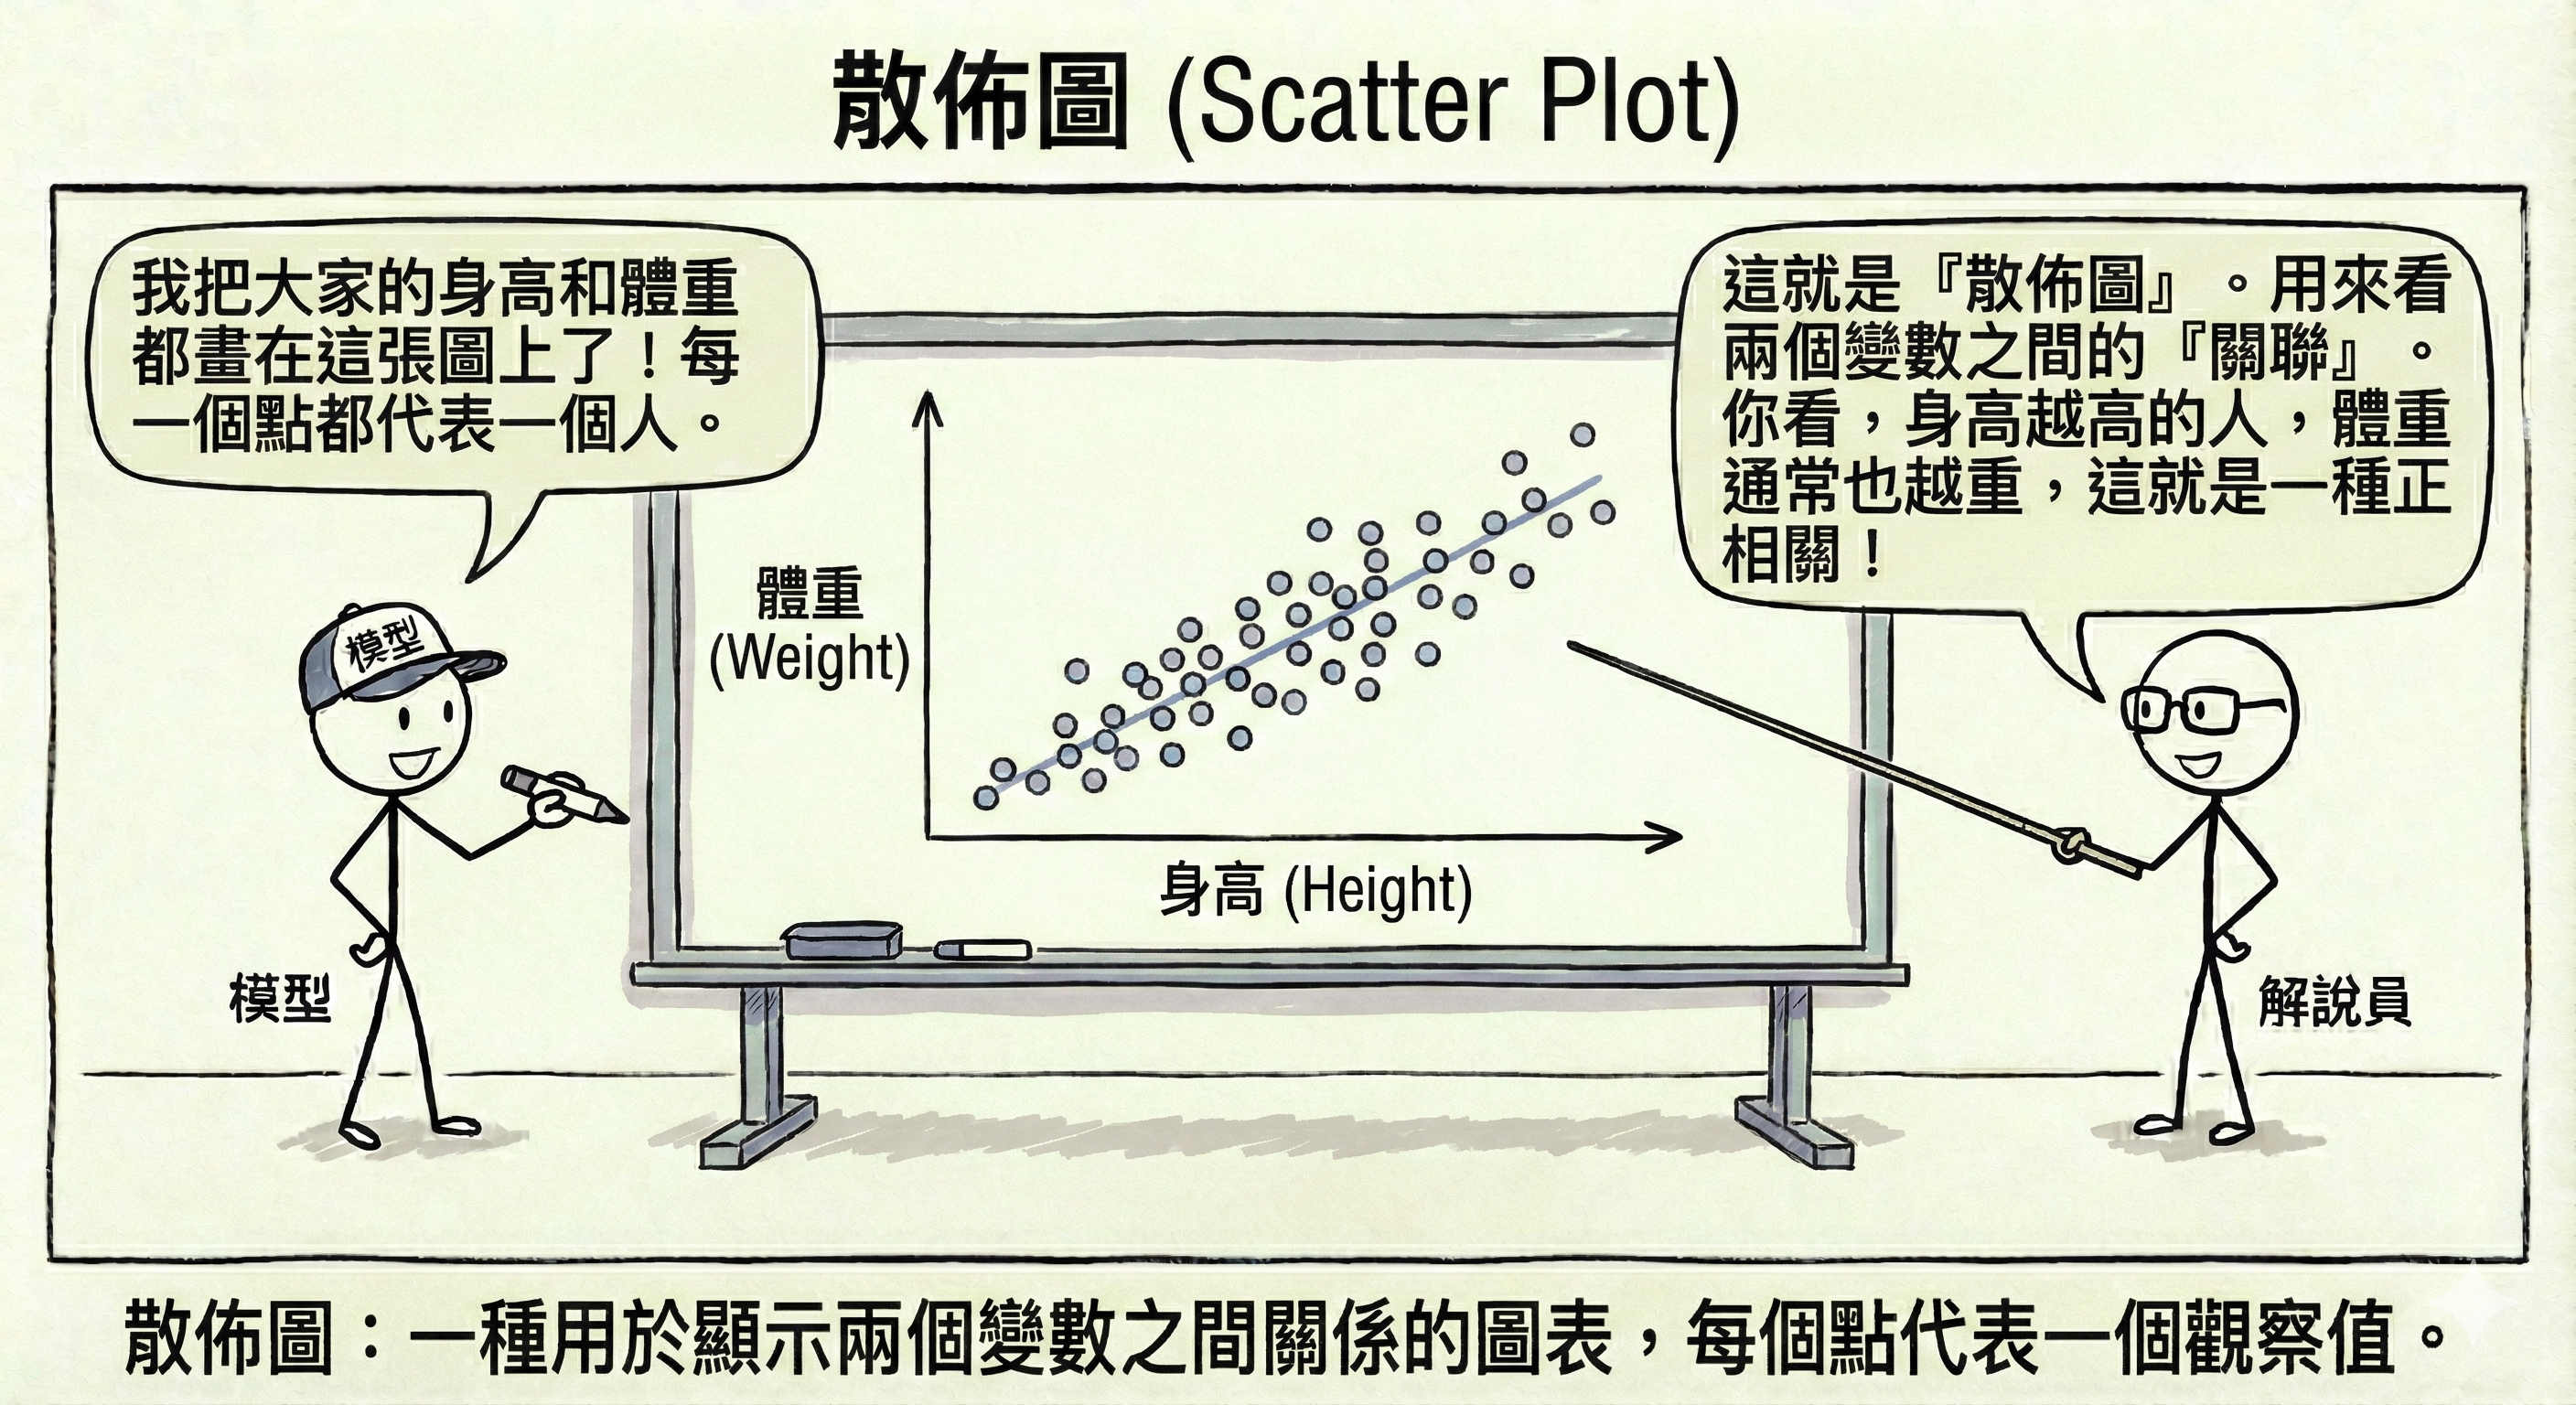
\includegraphics[keepaspectratio]{images/scatter-plot.png}}
\item
  \textbf{圓餅圖 (Pie
  Chart)}：顯示各類別佔整體的\textbf{比例}（例如：市佔率）。
  \pandocbounded{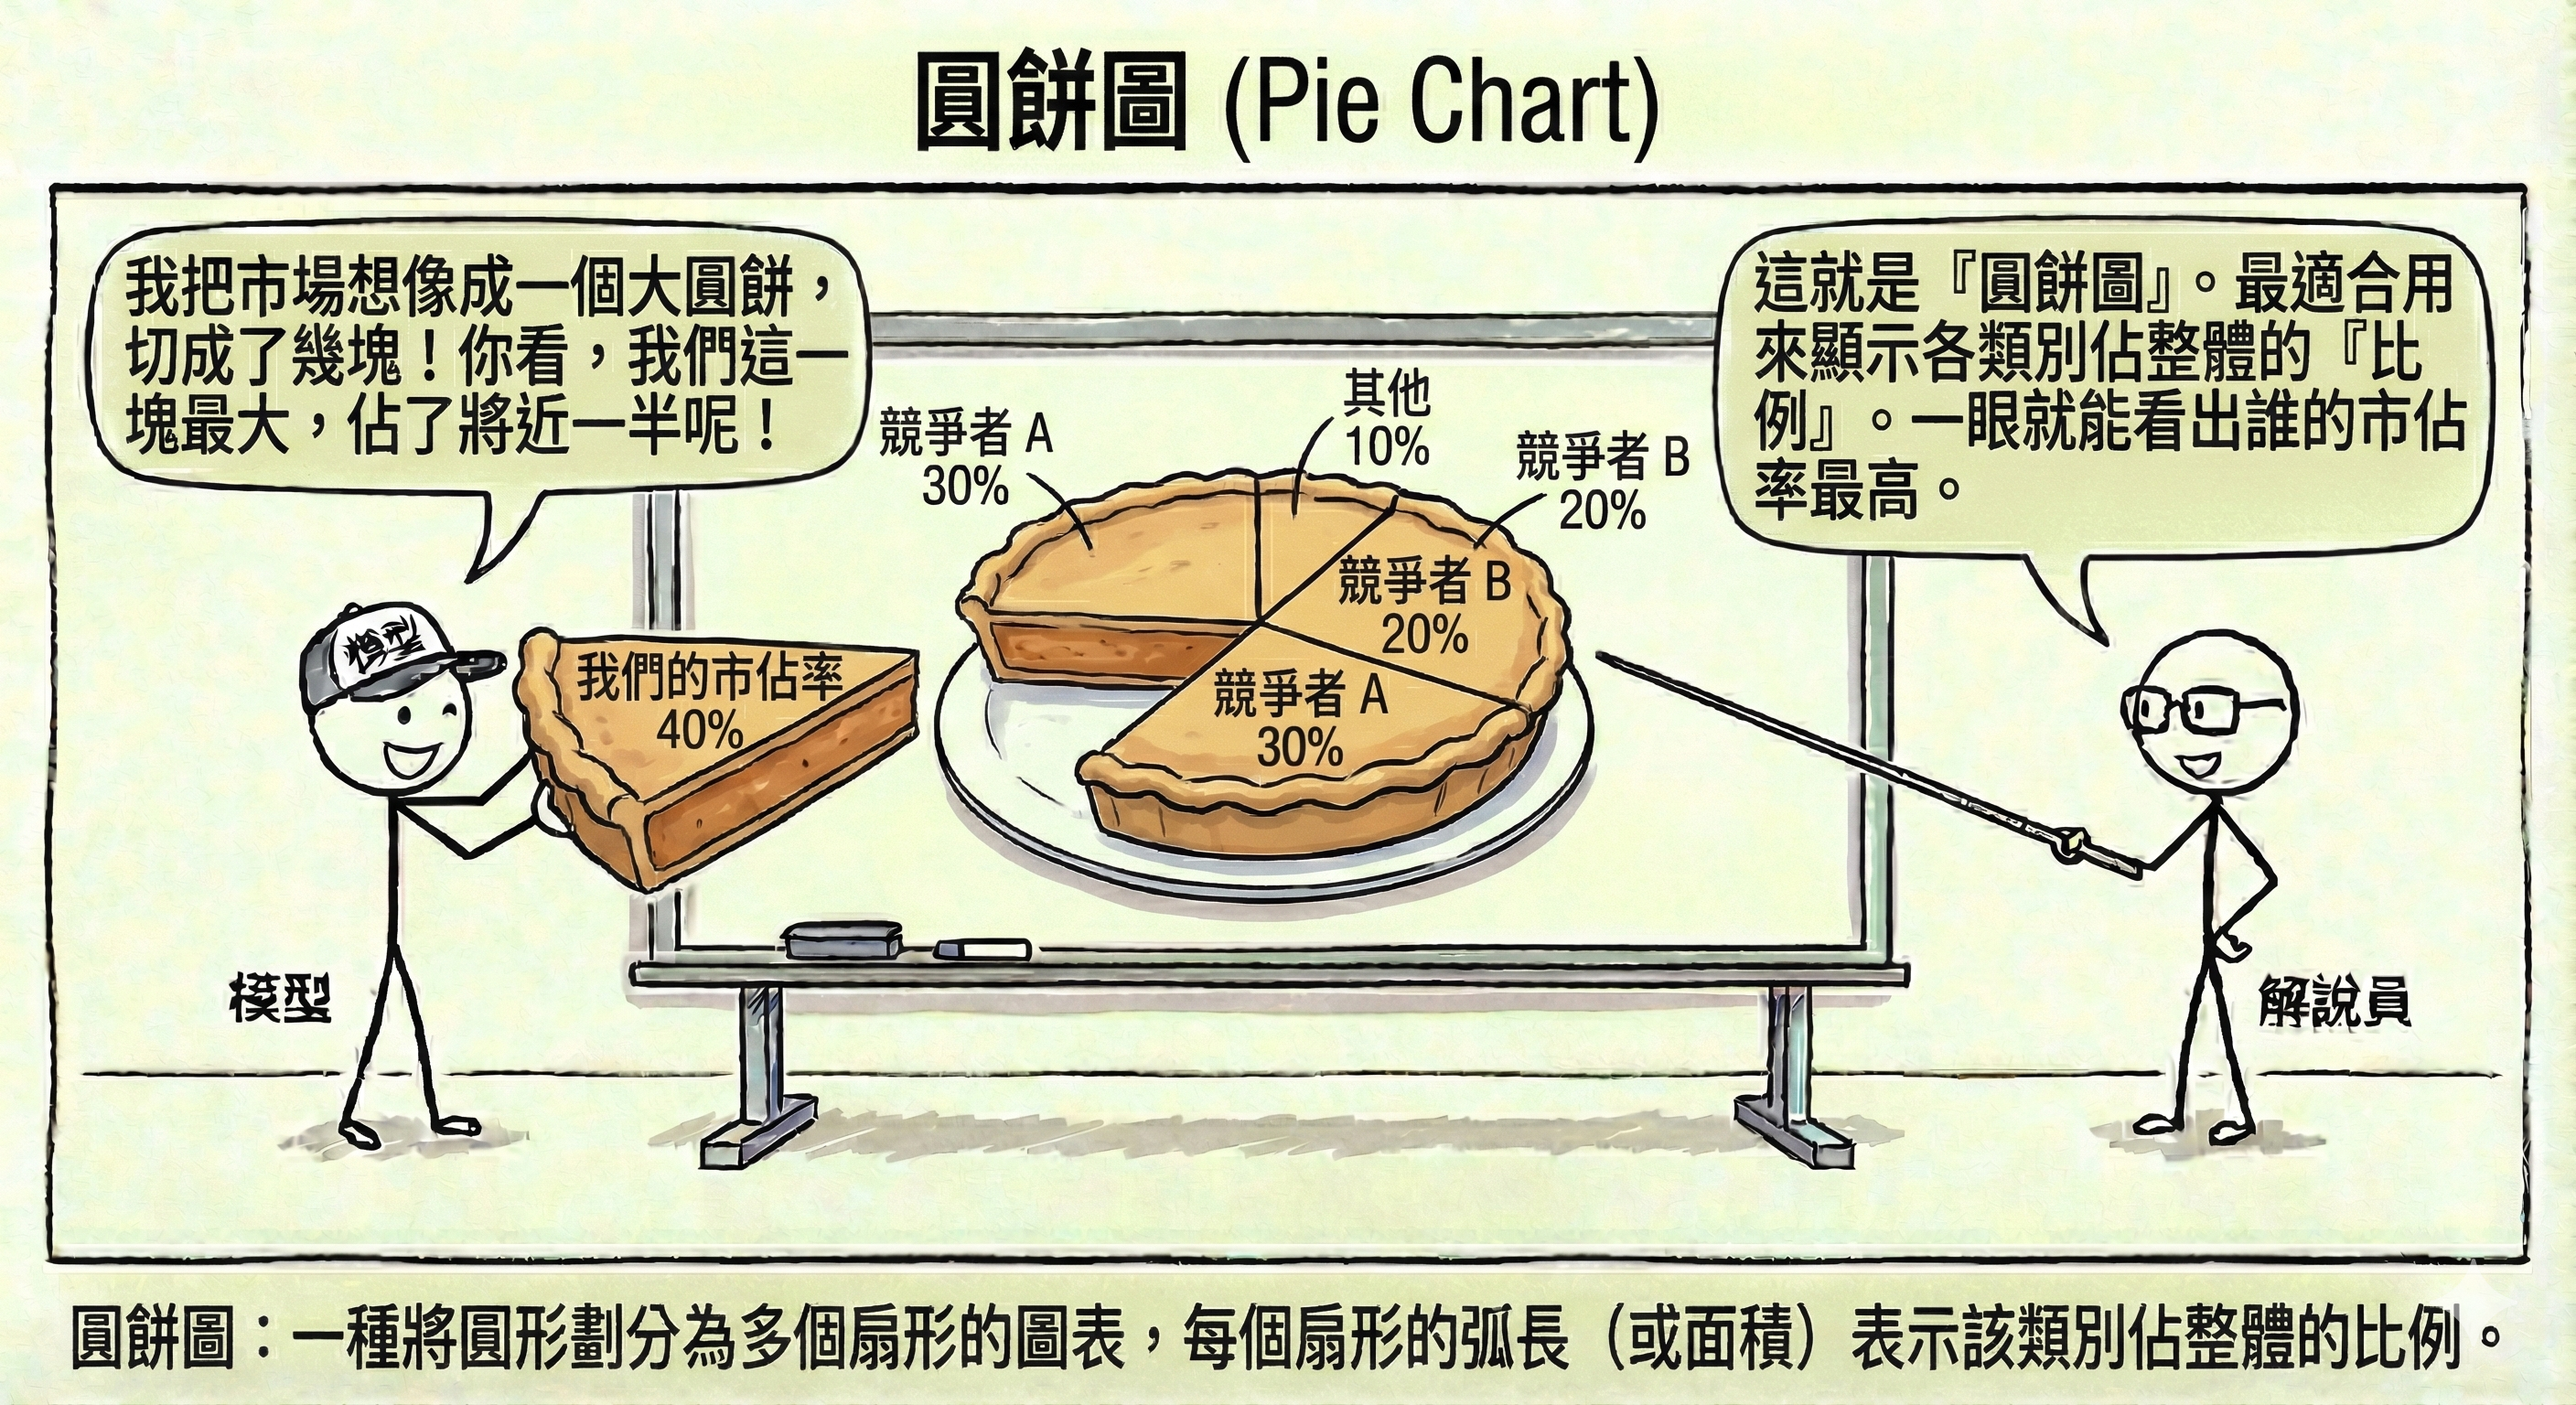
\includegraphics[keepaspectratio]{images/pie-chart.png}}
\item
  \textbf{折線圖 (Line
  Chart)}：看\textbf{時間趨勢}（例如：股價走勢、氣溫變化）。
  \pandocbounded{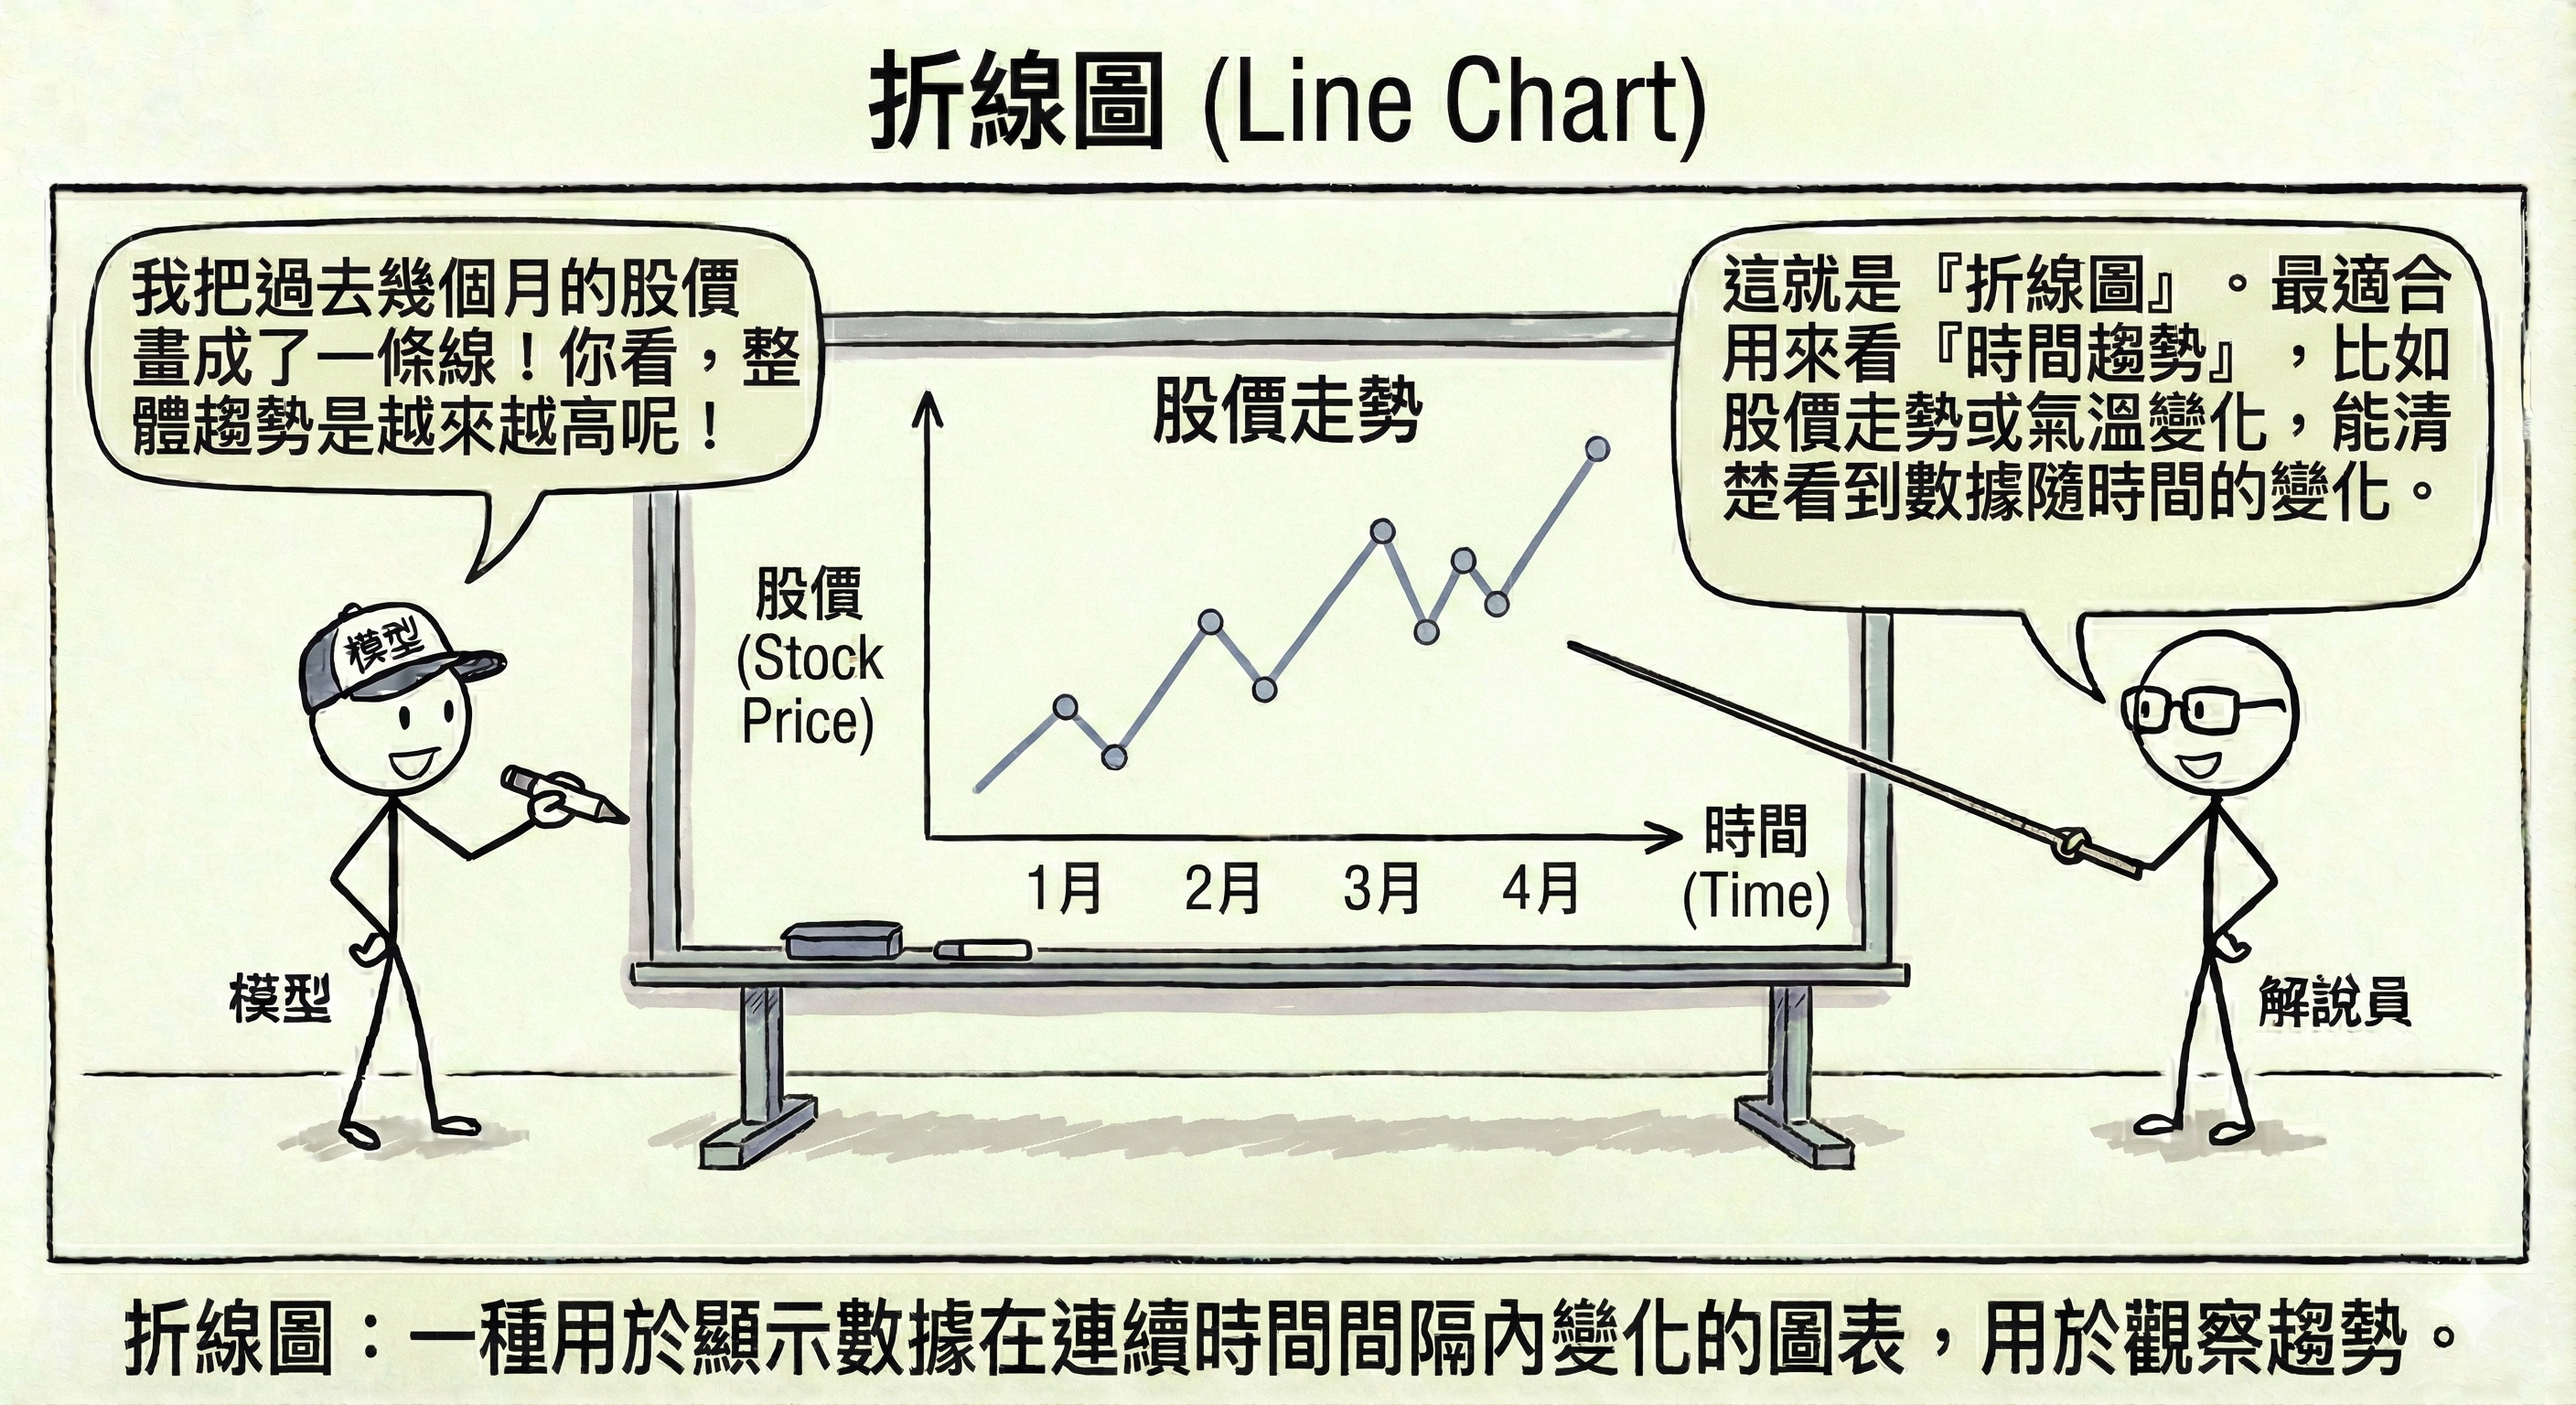
\includegraphics[keepaspectratio]{images/line-chart.png}}
\item
  \textbf{直方圖
  (Histogram)}：看單一變數的\textbf{分佈}情況（例如：全校學生的成績分佈）。
  \pandocbounded{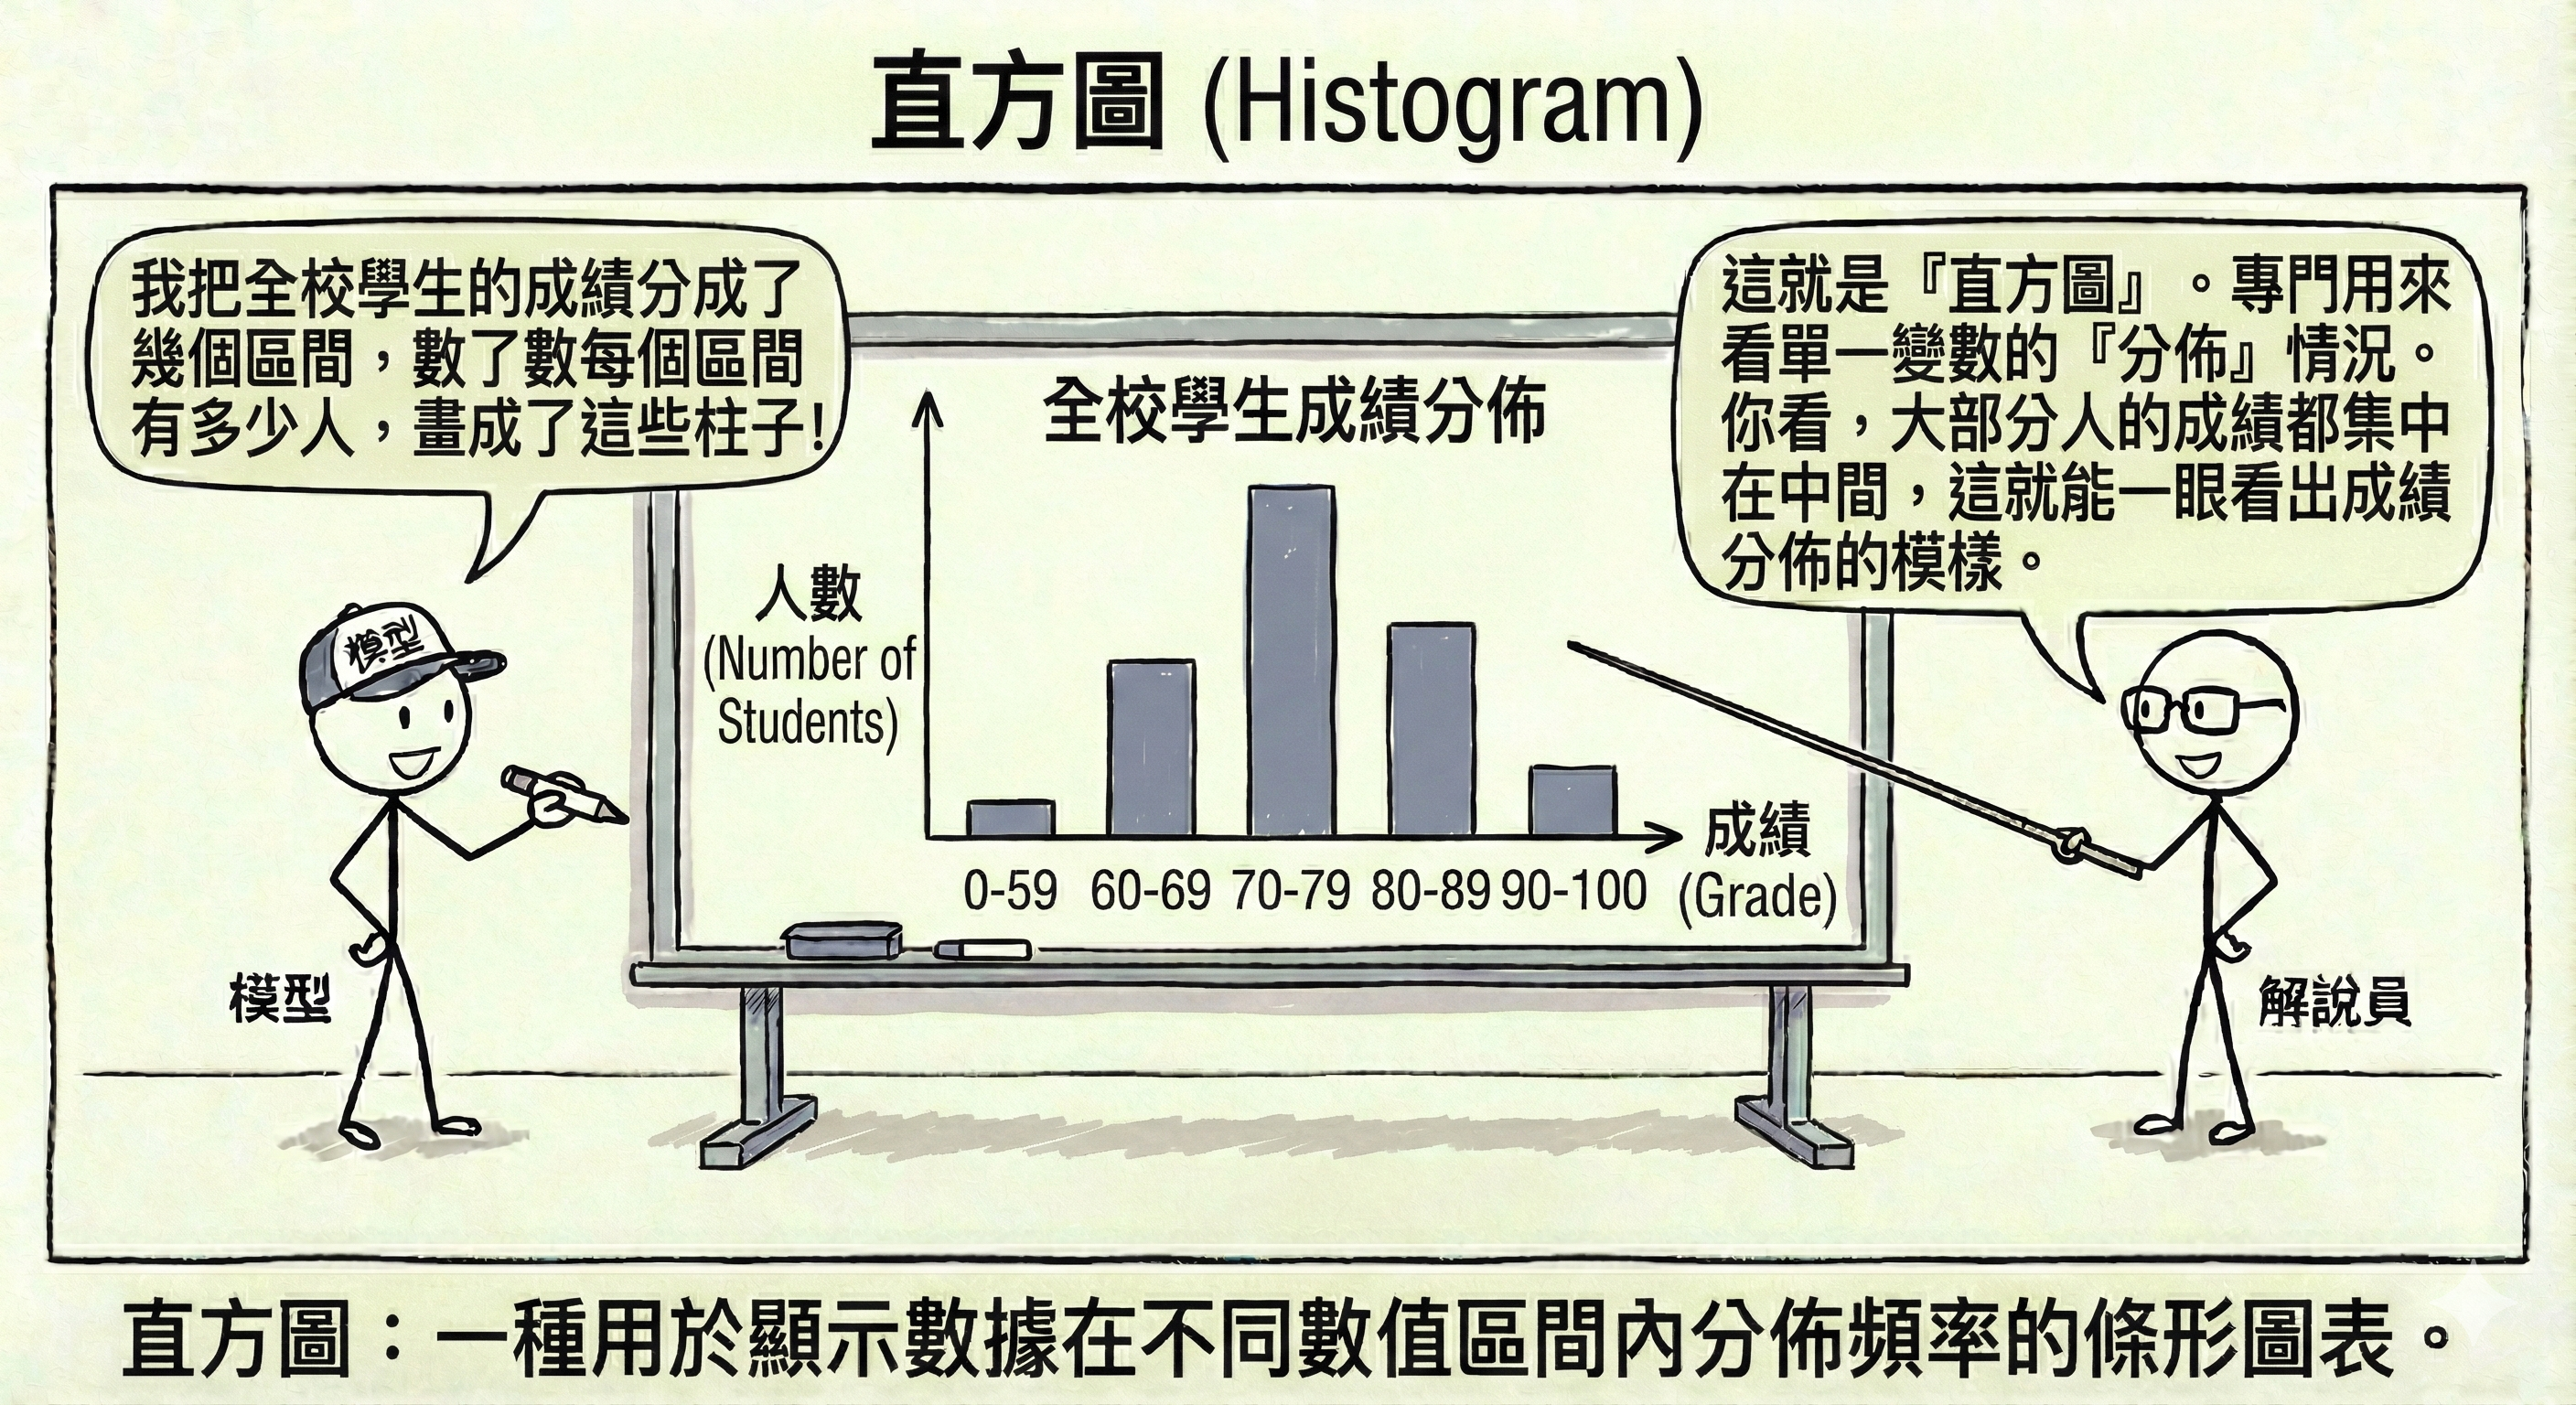
\includegraphics[keepaspectratio]{images/histogram.png}}
\item
  \textbf{長條圖 (Bar
  Chart)}：比較不同\textbf{類別}的大小（例如：各部門的業績比較）。
  \pandocbounded{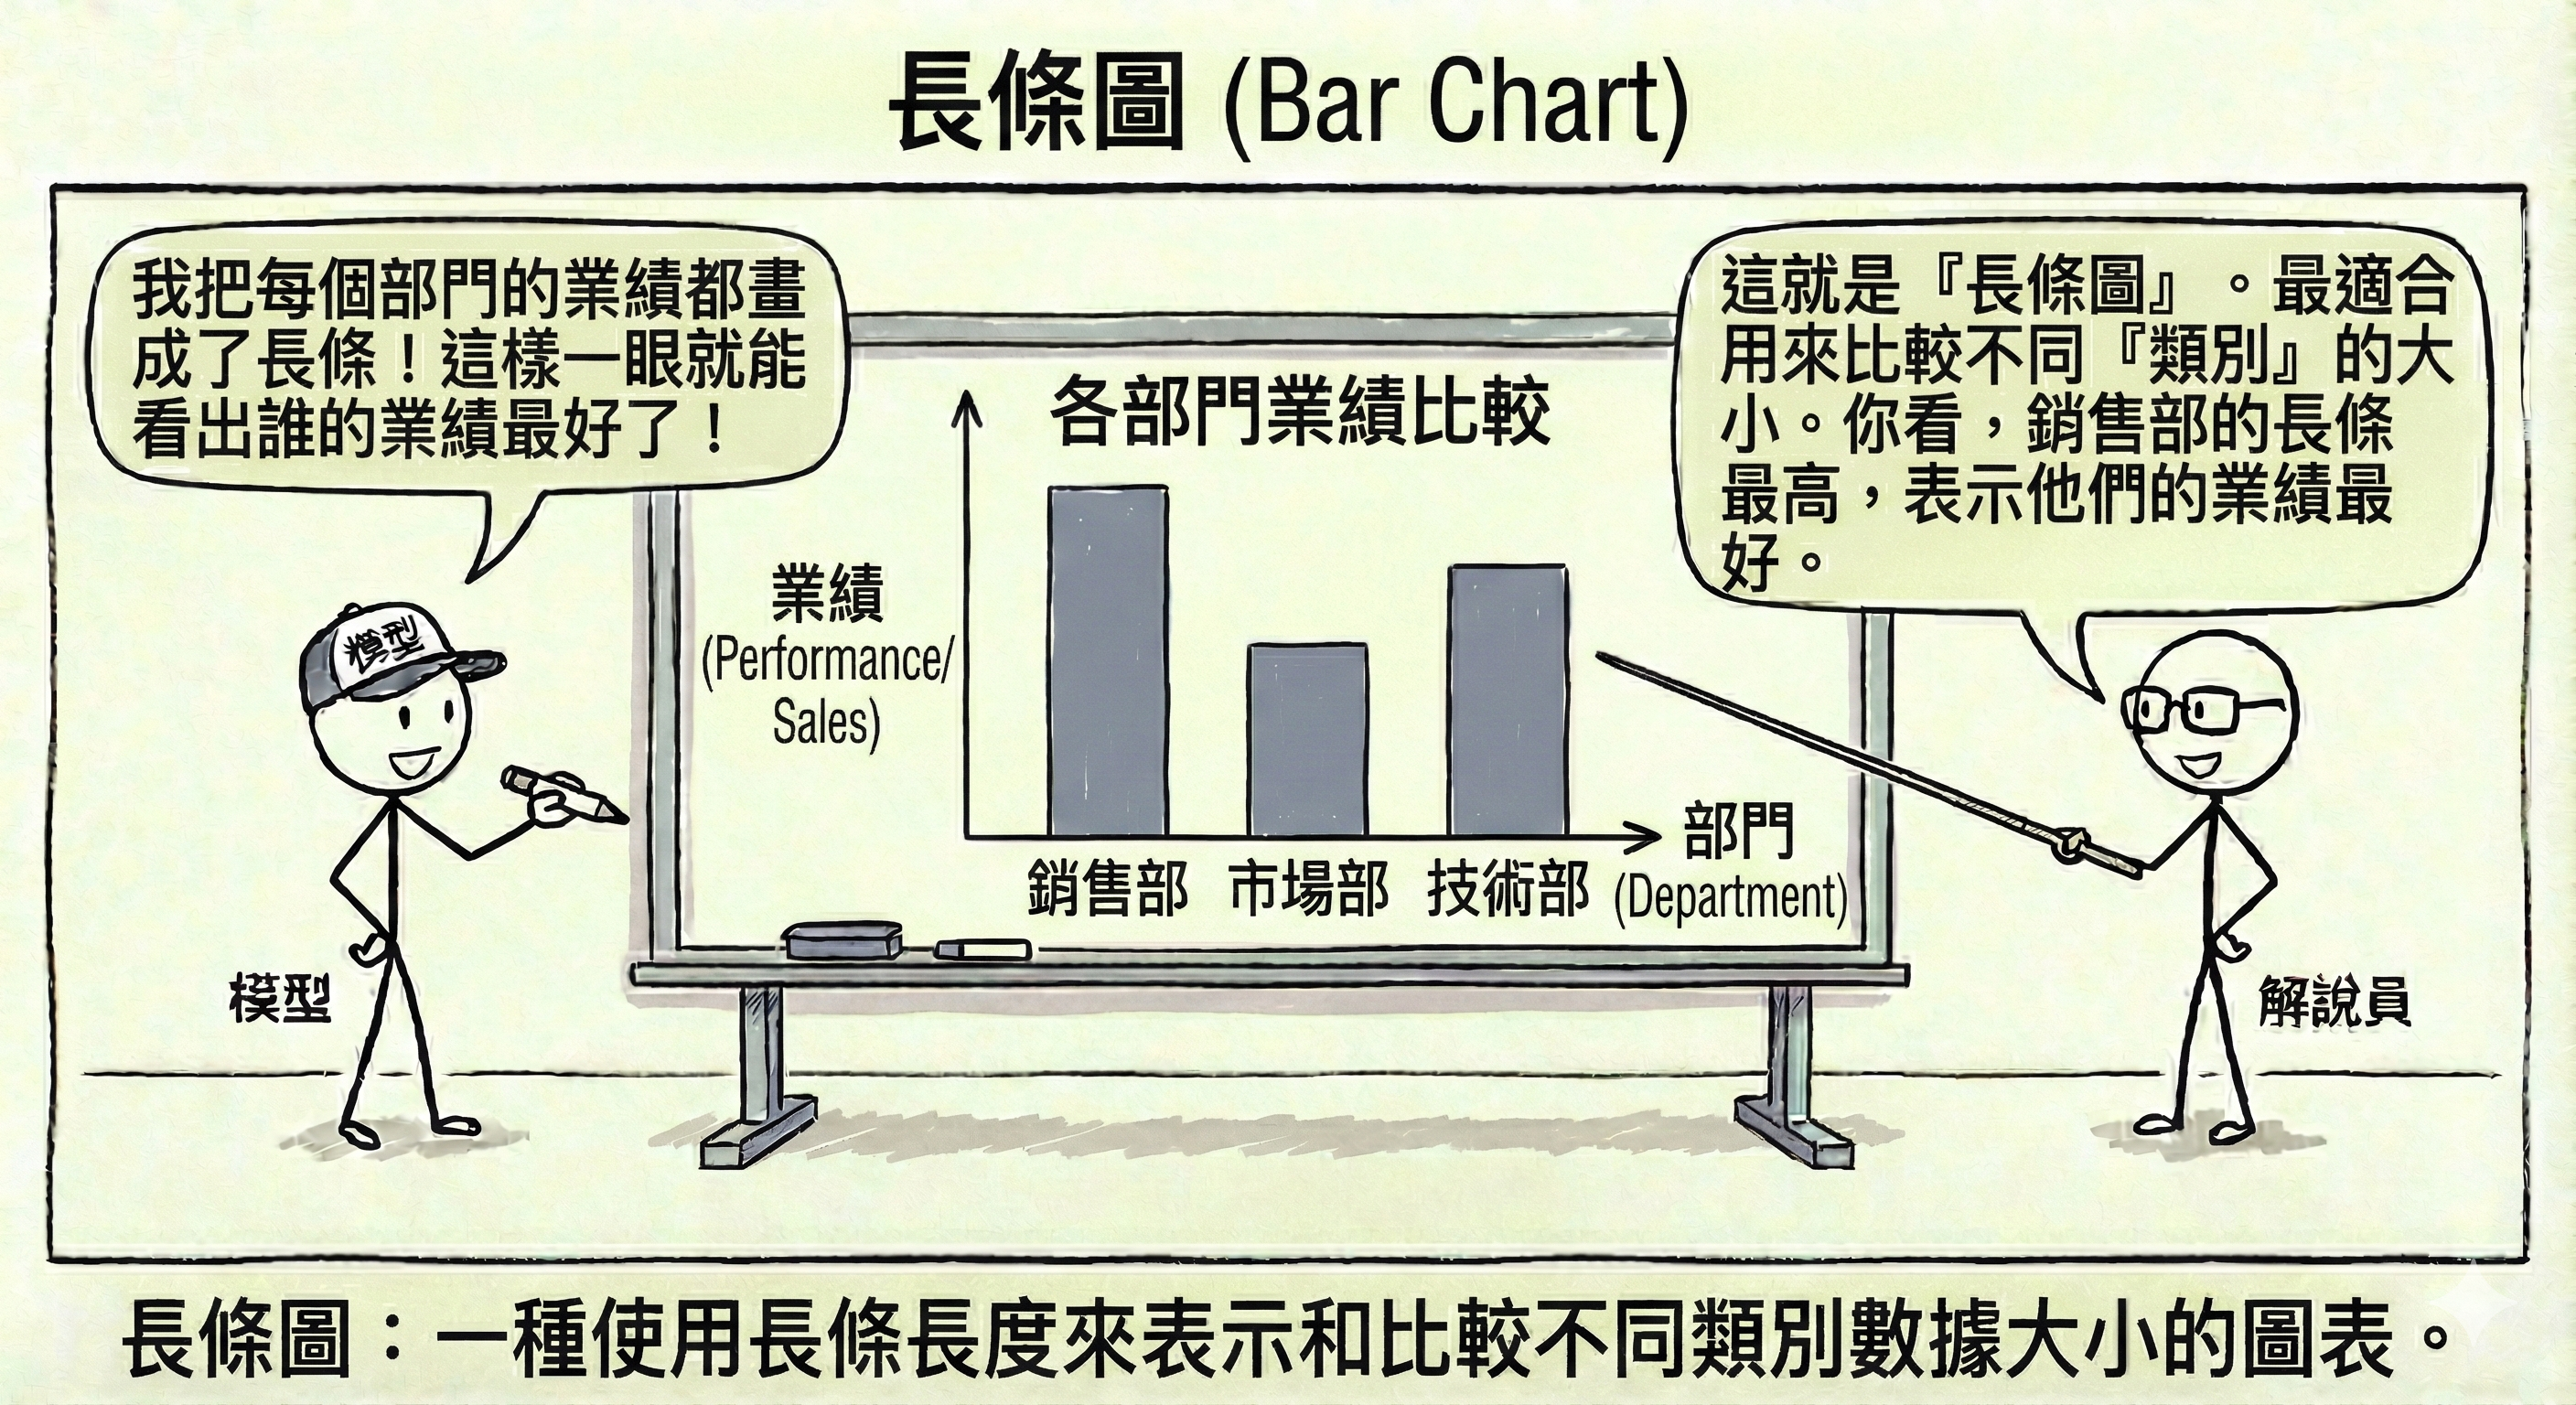
\includegraphics[keepaspectratio]{images/bar-chart.png}}
\item
  \textbf{熱圖
  (Heatmap)}：用顏色深淺表示數值大小，常用於顯示\textbf{相關係數矩陣}（哪些變數連動性高）。
  \pandocbounded{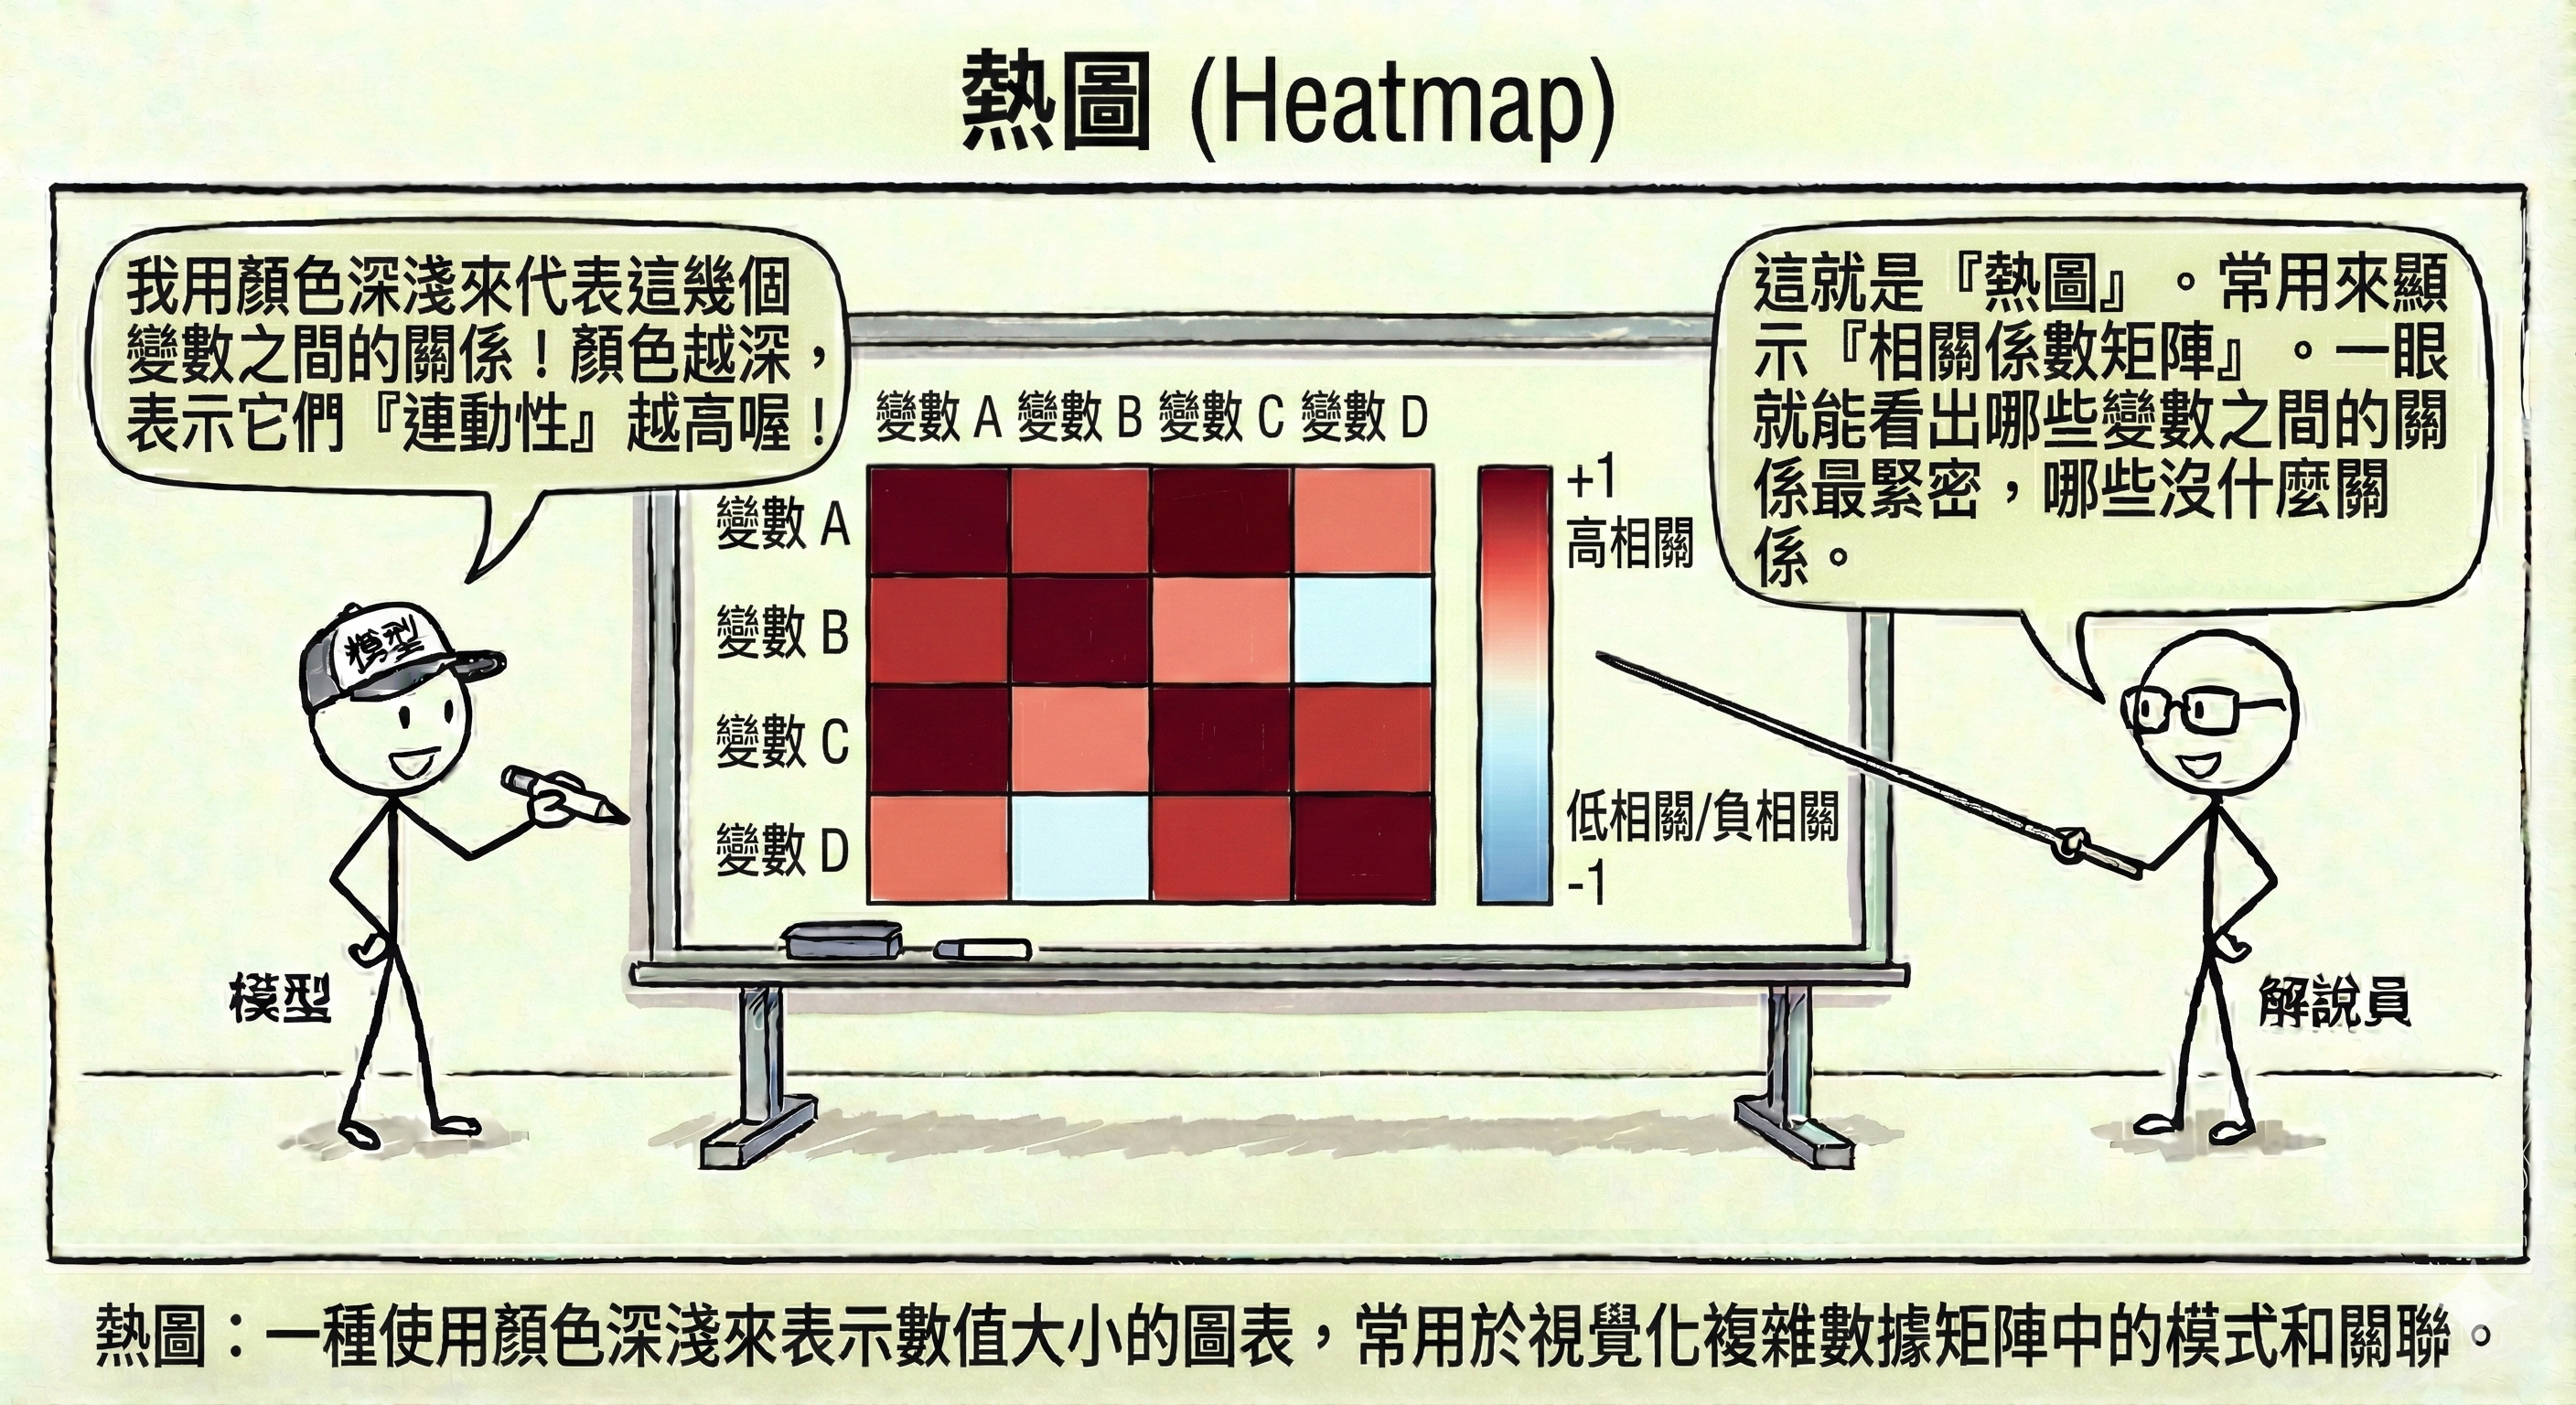
\includegraphics[keepaspectratio]{images/heatmap.png}}
\item
  \textbf{盒鬚圖 (Box
  Plot)}：快速看出資料的分佈範圍、中位數以及\textbf{離群值}。
  \pandocbounded{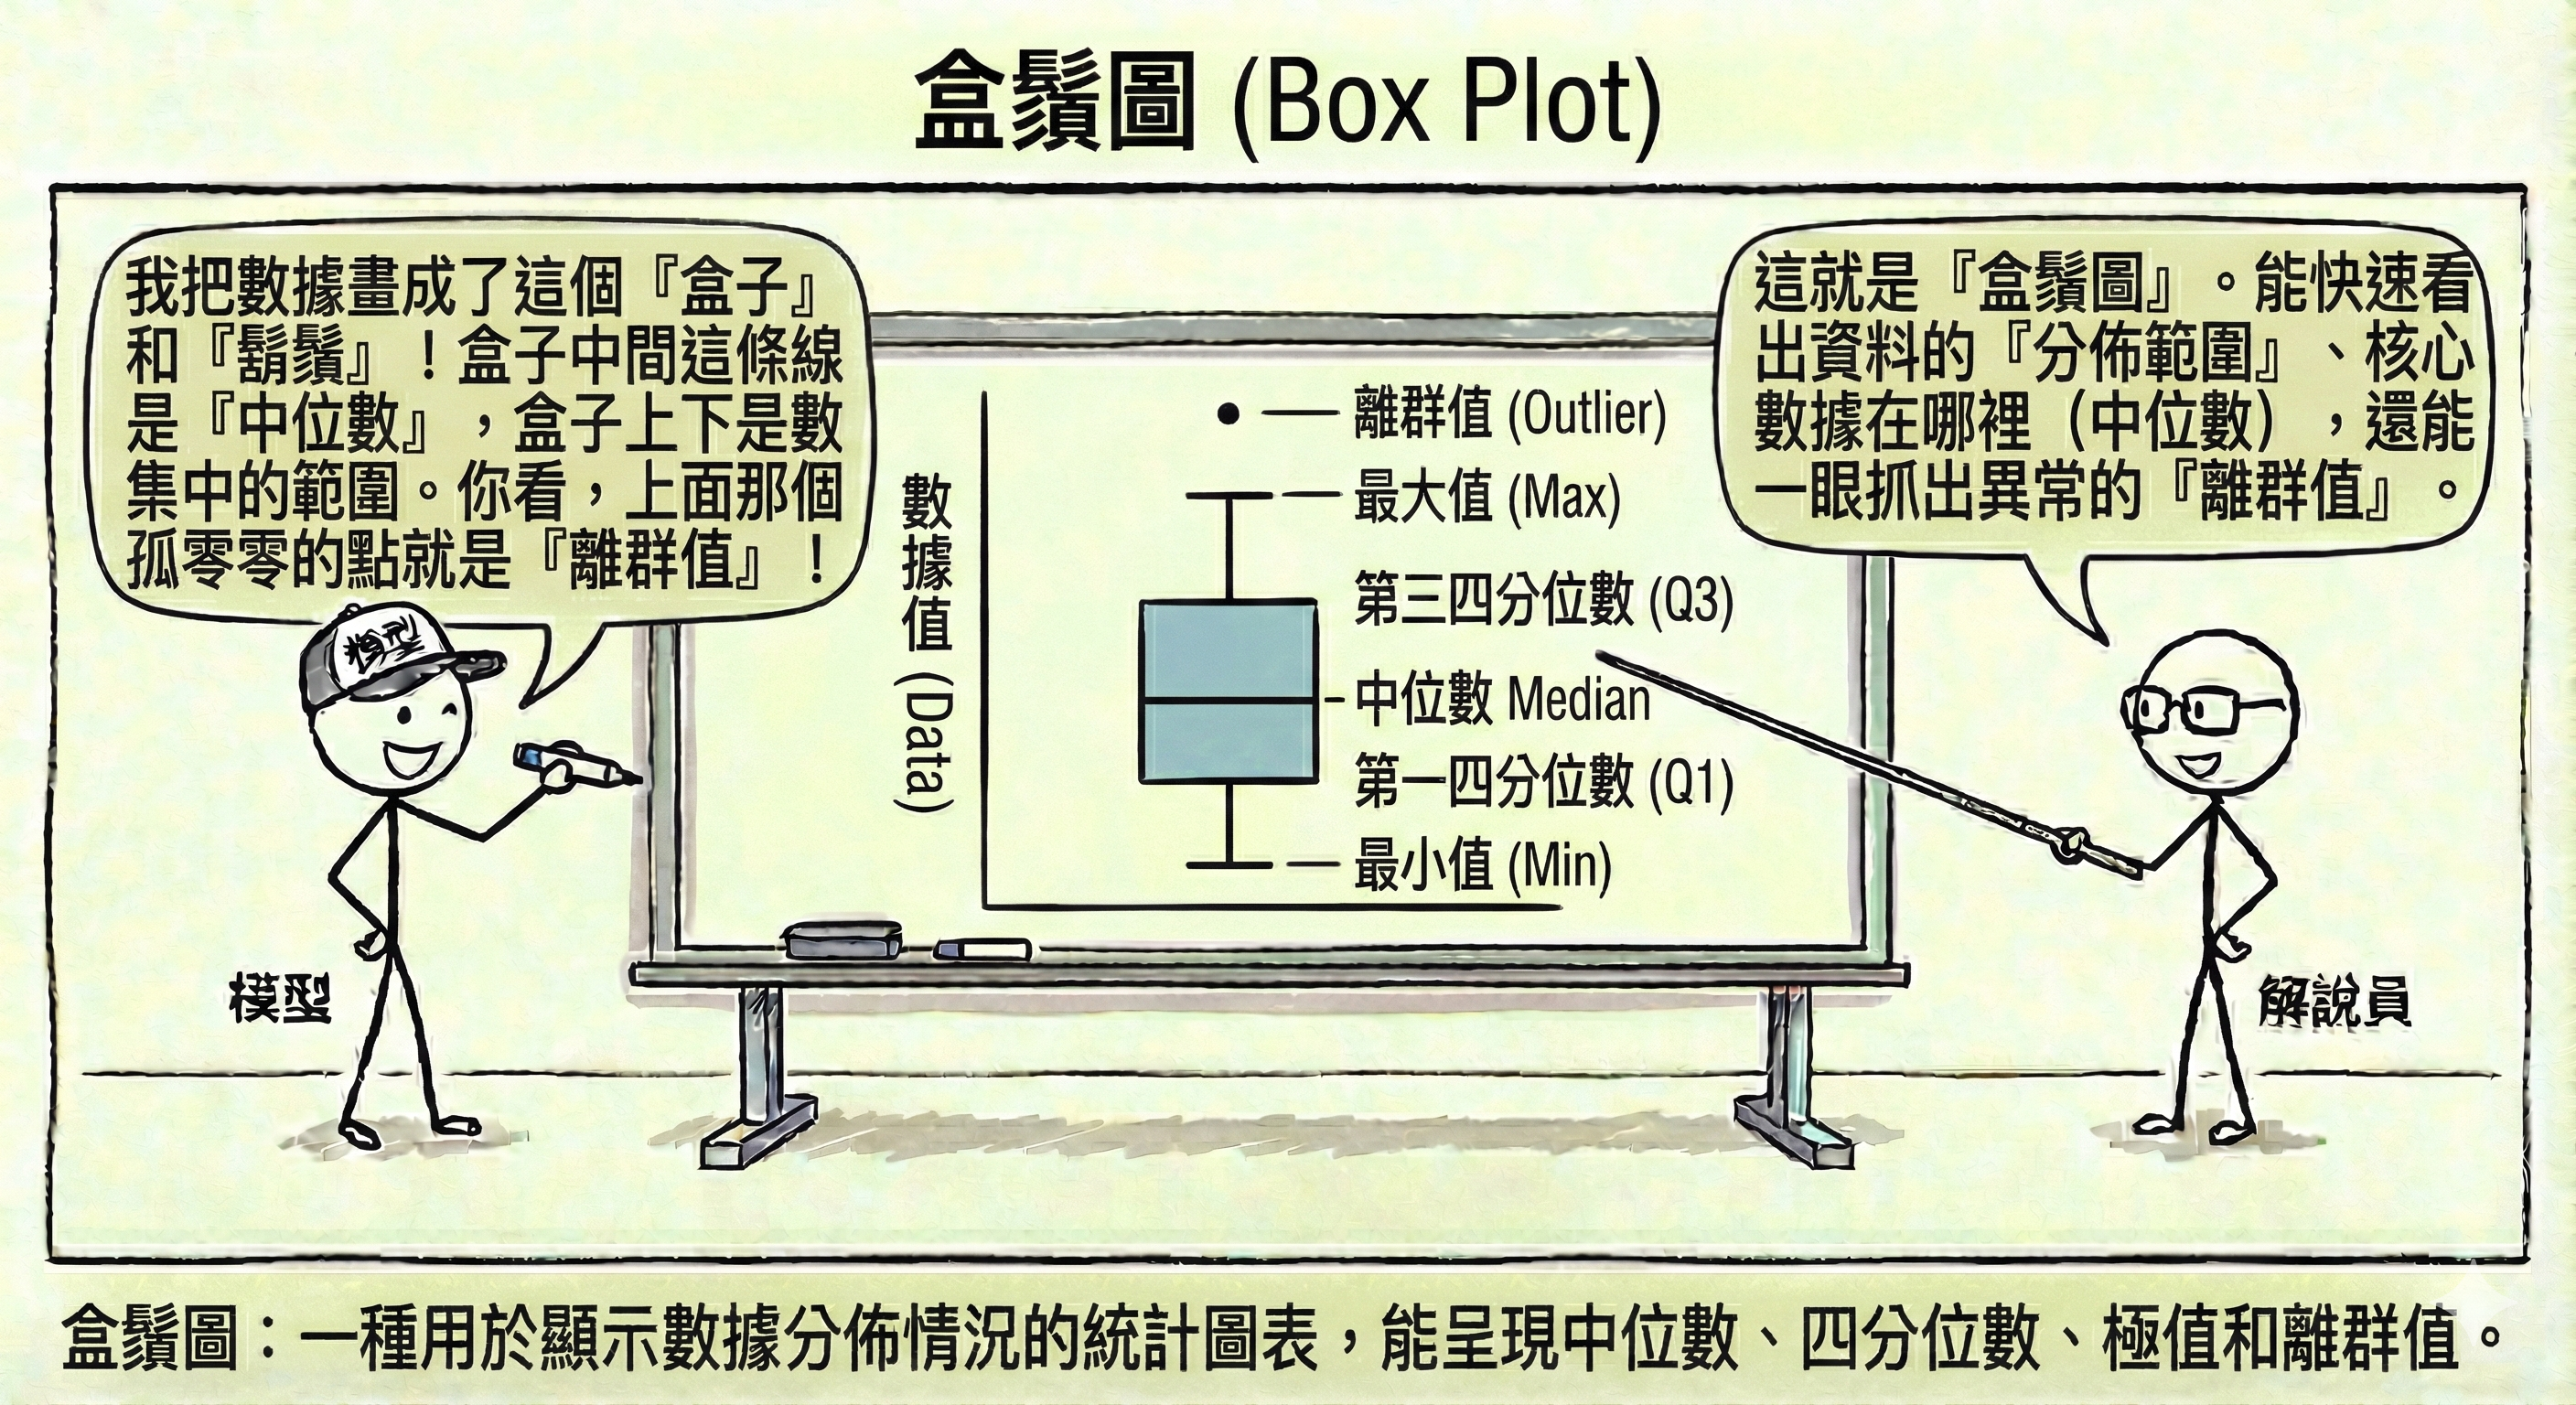
\includegraphics[keepaspectratio]{images/box-plot.png}}
\end{itemize}

\chapter{3.3 資料清理與品質管理}\label{sec-data-cleaning}

現實世界的資料往往是髒亂的。資料清理 (Data Cleaning) 通常佔據資料科學家
80\% 的時間。

\section{缺失值處理 (Missing Values)}\label{sec-missing-values}

資料中有空格怎麼辦？

\begin{itemize}
\tightlist
\item
  \textbf{刪除法}：如果缺失比例很低，直接刪除該筆資料。但可能會丟失重要資訊。
\item
  \textbf{插補法 (Imputation)}：用「猜」的。

  \begin{itemize}
  \tightlist
  \item
    用平均數、中位數填補（最簡單）。
  \item
    用機器學習模型預測缺失值（較精準）。
  \end{itemize}
\end{itemize}

\section{異常值/離群值處理 (Outliers)}\label{sec-outliers}

有些資料點明顯與眾不同，例如身高 300 公分的人，或是年齡 200 歲。

\begin{itemize}
\tightlist
\item
  \textbf{偵測方法}：

  \begin{itemize}
  \tightlist
  \item
    \textbf{Z-score}：超過平均數 3 個標準差以外的數值。
  \item
    \textbf{四分位距 (IQR)}：在盒鬚圖鬚鬚之外的點。
  \end{itemize}
\item
  \textbf{處理方式}：

  \begin{itemize}
  \tightlist
  \item
    如果是輸入錯誤（如年齡 200），直接修正或刪除。
  \item
    如果是真實存在的極端值（如億萬富翁的收入），可以使用\textbf{對數轉換
    (Log Transformation)} 來壓縮數值，減少其對模型的影響。
  \end{itemize}
\end{itemize}

\section{數據一致性處理}\label{sec-consistency}

\begin{itemize}
\tightlist
\item
  \textbf{欄位標準化}：將 ``Taipei'', ``Taipei City'', ``TP'' 統一為
  ``Taipei''。
\item
  \textbf{去重 (Deduplication)}：刪除重複的紀錄。
\end{itemize}

\section{資料匿名化與隱私保護 (PII 處理)}\label{sec-anonymization}

在處理涉及個人隱私 (PII, Personally Identifiable Information)
的資料時，必須進行去識別化。 * \textbf{遮罩 (Masking)}：將姓名顯示為
``王O明''。 * \textbf{泛化 (Generalization)}：將年齡 ``25 歲'' 改為
``20-30 歲區間''。

\part{特徵工程 (Feature
Engineering)}\label{ux7279ux5fb5ux5de5ux7a0b-feature-engineering}

特徵工程被認為是機器學習中「最像藝術」的部分。吳恩達 (Andrew Ng)
曾說：「數據就像原油，而特徵工程就是煉油的過程。」好的特徵工程能讓普通的模型表現出色，而糟糕的特徵工程則會讓頂尖的模型無用武之地。

\chapter{4.1 數值特徵處理}\label{sec-numerical-features}

數值資料（如身高、價格、次數）看似可以直接使用，但往往需要經過轉換才能發揮最大效用。

\section{特徵縮放 (Feature Scaling)}\label{sec-feature-scaling}

當不同特徵的單位或範圍差異很大時（例如：年齡 0-100，年薪
0-10,000,000），模型可能會被數值大的特徵主導，導致學習效果不佳。

\begin{itemize}
\tightlist
\item
  \textbf{標準化 (Standardization / Z-score Normalization)}：

  \begin{itemize}
  \tightlist
  \item
    將資料轉換為平均值為 0，標準差為 1 的分佈。
  \item
    \textbf{公式}：\(z = \frac{x - \mu}{\sigma}\)
  \item
    \textbf{適用}：大部分機器學習演算法（如 SVM, Logistic Regression,
    Neural Networks）。
  \end{itemize}
\item
  \textbf{正規化 (Normalization / Min-Max Scaling)}：

  \begin{itemize}
  \tightlist
  \item
    將資料壓縮到 {[}0, 1{]} 之間。
  \item
    \textbf{公式}：\(x_{new} = \frac{x - x_{min}}{x_{max} - x_{min}}\)
  \item
    \textbf{適用}：對範圍敏感的演算法，或影像處理（像素值 0-255）。
  \end{itemize}
\end{itemize}

\section{特徵轉換}\label{sec-feature-transformation}

\begin{itemize}
\tightlist
\item
  \textbf{對數轉換 (Log Transformation)}：

  \begin{itemize}
  \tightlist
  \item
    \textbf{目的}：處理\textbf{長尾分佈}或\textbf{偏態}資料（如收入、房價）。
  \item
    \textbf{效果}：將原本擠在一起的較小數值拉開，並壓縮極端大的數值，使分佈更接近常態分佈
    (Normal Distribution)。
  \end{itemize}
\item
  \textbf{特徵分箱 (Binning)}：

  \begin{itemize}
  \tightlist
  \item
    \textbf{目的}：將連續數值轉為區間類別。
  \item
    \textbf{例子}：將年齡 0-100
    歲轉為「兒童」、「青少年」、「成年」、「老年」。
  \item
    \textbf{效果}：減少微小數值波動的雜訊，增加模型的魯棒性。
  \end{itemize}
\end{itemize}

\chapter{4.2 類別特徵編碼}\label{sec-categorical-encoding}

機器學習模型通常只看得懂數字，看不懂文字。我們需要將類別資料（如顏色、城市）轉換為數字。

\begin{itemize}
\tightlist
\item
  \textbf{序數編碼 (Ordinal Encoding)}：

  \begin{itemize}
  \tightlist
  \item
    \textbf{適用}：類別之間有\textbf{順序}或\textbf{大小}關係。
  \item
    \textbf{例子}：衣服尺寸（S=1, M=2, L=3, XL=4）。
  \end{itemize}
\item
  \textbf{獨熱編碼 (One-hot Encoding)}：

  \begin{itemize}
  \tightlist
  \item
    \textbf{適用}：類別之間\textbf{沒有}順序關係。
  \item
    \textbf{例子}：顏色（紅、綠、藍）。
  \item
    \textbf{做法}：建立三個欄位，「是紅色嗎？」(1/0)、「是綠色嗎？」(1/0)、「是藍色嗎？」(1/0)。
  \item
    \textbf{缺點}：如果類別太多（如所有城市名），會產生過多欄位（維度災難）。
  \end{itemize}
\item
  \textbf{特徵嵌入 (Feature Embedding)}：

  \begin{itemize}
  \tightlist
  \item
    \textbf{適用}：高基數類別（類別數量極多）或文本。
  \item
    \textbf{做法}：將每個類別映射到一個低維度的向量空間（如
    Word2Vec），讓意義相近的類別在空間中距離較近。
  \end{itemize}
\end{itemize}

\chapter{4.3 進階特徵技巧}\label{sec-advanced-features}

\begin{itemize}
\tightlist
\item
  \textbf{特徵交叉 (Feature Cross)}：

  \begin{itemize}
  \tightlist
  \item
    將兩個或多個特徵組合起來，捕捉非線性的交互作用。
  \item
    \textbf{例子}：單看「地點」或「時間」可能無法預測計程車需求，但「地點
    x 時間」（例如：週五晚上的信義區）就是一個強特徵。
  \end{itemize}
\item
  \textbf{特徵選擇 (Feature Selection)}：

  \begin{itemize}
  \tightlist
  \item
    不是特徵越多越好。過多的特徵會導致\textbf{過度擬合 (Overfitting)}
    和計算量大增。
  \item
    \textbf{過濾法 (Filter)}：用統計方法（如相關係數）篩選。
  \item
    \textbf{包裝法 (Wrapper)}：直接用模型試跑，看哪些特徵效果好。
  \end{itemize}
\item
  \textbf{降維技術 (Dimensionality Reduction)}：

  \begin{itemize}
  \tightlist
  \item
    \textbf{主成分分析
    (PCA)}：將高維度資料投影到低維度空間，保留變異量最大的方向。就像把立體的物體拍成平面照片，盡量保留其形狀特徵。
  \end{itemize}
\end{itemize}

\chapter{4.4 不平衡資料處理 (Imbalanced
Data)}\label{sec-imbalanced-data}

在詐欺偵測或罕見疾病診斷中，正樣本（詐欺、患病）通常極少（例如
1\%），負樣本極多（99\%）。模型容易傾向全部猜「正常」，雖然準確率高達
99\%，但完全沒用。

\begin{itemize}
\tightlist
\item
  \textbf{重採樣技術 (Resampling)}：

  \begin{itemize}
  \tightlist
  \item
    \textbf{過採樣 (Oversampling)}：複製少數類別的樣本，使其數量增加。
  \item
    \textbf{欠採樣
    (Undersampling)}：隨機刪除多數類別的樣本，使其數量減少。
  \end{itemize}
\item
  \textbf{合成樣本生成 (SMOTE)}：

  \begin{itemize}
  \tightlist
  \item
    不是單純複製，而是透過演算法在少數類別樣本之間「創造」出新的人工樣本，增加資料的多樣性。
  \end{itemize}
\item
  \textbf{類別權重調整 (Class Weights)}：

  \begin{itemize}
  \tightlist
  \item
    在訓練模型時，告訴模型：「答錯少數類別的懲罰，是答錯多數類別的 100
    倍。」強迫模型重視少數類別。
  \end{itemize}
\end{itemize}

\part{第三部：機器學習演算法核心}

\part{監督式學習演算法}\label{ux76e3ux7763ux5f0fux5b78ux7fd2ux6f14ux7b97ux6cd5}

監督式學習 (Supervised Learning) 是目前 AI
應用最成熟的領域。它的核心在於：給定輸入 \(X\) 和正確答案
\(Y\)，尋找一個函數 \(f\)，使得 \(f(X) \approx Y\)。根據 \(Y\)
的型態，又分為\textbf{分類}（預測類別）與\textbf{迴歸}（預測數值）。

\chapter{5.1 分類演算法 (Classification)}\label{sec-classification}

目標是將資料分門別類。

\section{K-近鄰演算法 (KNN, K-Nearest Neighbors)}\label{sec-knn}

\begin{itemize}
\tightlist
\item
  \textbf{概念}：「近朱者赤，近墨者黑」。想知道一個新資料點是哪一類，就看它最近的
  \(K\) 個鄰居是誰。如果鄰居大多是紅色，它就是紅色。
\item
  \textbf{特點}：簡單直觀，不需要訓練（Lazy
  Learning），但在資料量大時計算距離很慢。
\end{itemize}

\section{貝氏分類器 (Naive Bayes)}\label{sec-naive-bayes}

\begin{itemize}
\tightlist
\item
  \textbf{概念}：基於\textbf{機率}的預測。利用貝氏定理計算在已知特徵下，屬於某類別的機率。
\item
  \textbf{假設}：假設所有特徵之間是\textbf{獨立}的（這也是為什麼叫
  ``Naive'' 樸素/天真的原因）。
\item
  \textbf{應用}：垃圾郵件過濾（出現 ``中獎''、``匯款''
  等詞彙時，是垃圾信的機率）。
\end{itemize}

\section{邏輯迴歸 (Logistic Regression)}\label{sec-logistic-regression}

\begin{itemize}
\tightlist
\item
  \textbf{注意}：雖然名字裡有「迴歸」，但它是用來做\textbf{分類}的！
\item
  \textbf{概念}：將線性迴歸的結果通過一個 \textbf{Sigmoid
  函數}，將數值壓縮到 0 到 1 之間，代表「屬於某類別的機率」。
\item
  \textbf{決策邊界}：通常以 0.5 為界，大於 0.5 判為 1，小於 0.5 判為 0。
\end{itemize}

\section{支援向量機 (SVM, Support Vector Machine)}\label{sec-svm}

\begin{itemize}
\tightlist
\item
  \textbf{概念}：試圖在不同類別的資料之間，畫出一條最寬的「馬路」（決策邊界）。馬路越寬，容錯率越高，模型越穩健。
\item
  \textbf{核函數 (Kernel
  Trick)}：當資料在二維平面上無法用直線分開時（例如同心圓分佈），SVM
  可以將資料投影到高維空間（三維），用一個平面將其切開。這就像是把一張紙捲起來，就能讓原本相隔很遠的點碰在一起。
\end{itemize}

\section{決策樹 (Decision Tree)}\label{sec-decision-tree}

\begin{itemize}
\tightlist
\item
  \textbf{概念}：就像玩「20
  個問題」遊戲。透過一系列的是非問句來對資料進行分類。
\item
  \textbf{結構}：

  \begin{itemize}
  \tightlist
  \item
    \textbf{根節點}：第一個問題。
  \item
    \textbf{葉節點}：最終的分類結果。
  \end{itemize}
\item
  \textbf{優點}：可解釋性高，畫出來的樹狀圖人類容易理解。
\item
  \textbf{缺點}：容易\textbf{過度擬合
  (Overfitting)}，把雜訊也當成規則學進去了（死記硬背）。
\end{itemize}

\section{隨機森林 (Random Forest)}\label{sec-random-forest}

\begin{itemize}
\tightlist
\item
  \textbf{概念}：\textbf{集成學習 (Ensemble Learning)}
  的代表。既然一棵樹容易犯錯，那就種一片森林！
\item
  \textbf{Bagging}：訓練多棵決策樹，每棵樹只看部分的資料和部分的特徵。最終結果由所有樹\textbf{投票}決定（少數服從多數）。
\item
  \textbf{優勢}：準確率高，不易過度擬合。
\end{itemize}

\chapter{5.2 迴歸演算法 (Regression)}\label{sec-regression}

目標是預測一個連續的數值。

\section{線性迴歸 (Linear Regression)}\label{sec-linear-regression}

\begin{itemize}
\tightlist
\item
  \textbf{概念}：試圖畫出一條直線，讓這條線盡可能靠近所有的資料點。
\item
  \textbf{最小平方法 (Least
  Squares)}：計算所有點到線的距離平方和，找出讓這個和最小的那條線。
\end{itemize}

\section{正規化迴歸 (Regularized
Regression)}\label{sec-regularized-regression}

為了防止模型過度擬合（Overfitting），我們在損失函數中加入一個「懲罰項」，強迫模型的權重不要太大，保持簡單。

\begin{itemize}
\tightlist
\item
  \textbf{L1 正則化 (Lasso)}：

  \begin{itemize}
  \tightlist
  \item
    傾向於讓不重要的特徵權重\textbf{變成 0}。
  \item
    \textbf{功能}：自動進行\textbf{特徵選擇}，得到稀疏模型 (Sparse
    Model)。
  \end{itemize}
\item
  \textbf{L2 正則化 (Ridge)}：

  \begin{itemize}
  \tightlist
  \item
    傾向於讓所有特徵權重\textbf{變小}，但不會變成 0。
  \item
    \textbf{功能}：處理共線性問題（特徵之間高度相關），讓模型更穩定。
  \end{itemize}
\end{itemize}

\part{非監督式學習與強化學習}\label{ux975eux76e3ux7763ux5f0fux5b78ux7fd2ux8207ux5f37ux5316ux5b78ux7fd2}

非監督式學習 (Unsupervised Learning) 就像是讓 AI
在沒有老師的情況下自學，尋找資料中的隱藏結構。而強化學習 (Reinforcement
Learning) 則是讓 AI 像生物一樣，透過與環境互動、嘗試錯誤來學習生存策略。

\chapter{6.1 分群演算法 (Clustering)}\label{sec-clustering}

分群的目標是「物以類聚」，將相似的資料點歸為同一群。

\section{K-means 演算法}\label{sec-kmeans}

\begin{itemize}
\tightlist
\item
  \textbf{概念}：隨機選定 \(K\)
  個中心點（質心），然後不斷調整這些中心點的位置，直到每一群的內部差異最小。
\item
  \textbf{步驟}：

  \begin{enumerate}
  \def\labelenumi{\arabic{enumi}.}
  \tightlist
  \item
    隨機決定 \(K\) 個中心。
  \item
    將每個資料點分配給最近的中心。
  \item
    重新計算每一群的平均位置，作為新的中心。
  \item
    重複步驟 2-3，直到中心不再移動。
  \end{enumerate}
\item
  \textbf{缺點}：必須事先決定 \(K\) 值（要分幾群？）；對離群值敏感。
\end{itemize}

\section{階層式分群 (Hierarchical
Clustering)}\label{sec-hierarchical-clustering}

\begin{itemize}
\tightlist
\item
  \textbf{概念}：建立一個樹狀結構（Dendrogram），不需要事先決定 \(K\)
  值。
\item
  \textbf{做法}：

  \begin{itemize}
  \tightlist
  \item
    \textbf{聚合式
    (Agglomerative)}：一開始每個點都是一群，然後慢慢把最近的兩群合併，直到剩下一大群。
  \item
    \textbf{分裂式 (Divisive)}：一開始所有點是一大群，然後慢慢切分。
  \end{itemize}
\end{itemize}

\section{DBSCAN (Density-Based Spatial Clustering of Applications with
Noise)}\label{sec-dbscan}

\begin{itemize}
\tightlist
\item
  \textbf{概念}：基於\textbf{密度}的分群。只要點夠密集就算同一群，如果不夠密集就被視為雜訊。
\item
  \textbf{優勢}：可以找出任意形狀的群聚（不像 K-means
  傾向於圓形），且能自動識別並排除\textbf{離群值}。
\end{itemize}

\chapter{6.2 關聯規則與降維}\label{sec-association-rules}

\section{Apriori 演算法 (購物籃分析)}\label{sec-apriori}

\begin{itemize}
\tightlist
\item
  \textbf{經典案例}：「啤酒與尿布」。沃爾瑪發現週五晚上買尿布的爸爸，通常也會順便買啤酒。
\item
  \textbf{指標}：

  \begin{itemize}
  \tightlist
  \item
    \textbf{支持度 (Support)}：某個商品組合出現的頻率（例如：10\%
    的訂單同時有 A 和 B）。
  \item
    \textbf{信心度 (Confidence)}：買了 A 的人，有多大概率也會買
    B（例如：買尿布的人有 70\% 會買啤酒）。
  \item
    \textbf{提升度 (Lift)}：A 的出現是否有助於 B 的出現（Lift
    \textgreater{} 1 代表正相關，Lift \textless{} 1 代表負相關）。
  \end{itemize}
\end{itemize}

\section{主成分分析 (PCA)}\label{sec-pca}

（參見 4.3 節）PCA
也是一種非監督式學習，用於找出資料的主要變異方向，進行降維。

\section{自動編碼器 (Autoencoder)}\label{sec-autoencoder}

\begin{itemize}
\tightlist
\item
  \textbf{概念}：訓練一個神經網路，讓輸出等於輸入。
\item
  \textbf{結構}：

  \begin{itemize}
  \tightlist
  \item
    \textbf{編碼器 (Encoder)}：將輸入壓縮成低維度的「潛在表示 (Latent
    Representation)」。
  \item
    \textbf{解碼器 (Decoder)}：將潛在表示還原回原始輸入。
  \end{itemize}
\item
  \textbf{用途}：資料壓縮、去噪（Denoising）、異常偵測（如果還原不回來，代表是異常資料）。
\end{itemize}

\chapter{6.3 強化學習 (Reinforcement
Learning)}\label{sec-reinforcement-learning-detail}

強化學習是 AI 邁向自主決策的關鍵。

\section{核心要素}\label{sec-rl-elements}

\begin{itemize}
\tightlist
\item
  \textbf{代理人 (Agent)}：學習的主角（如瑪利歐）。
\item
  \textbf{環境 (Environment)}：遊戲關卡。
\item
  \textbf{狀態 (State)}：瑪利歐的位置、敵人的位置。
\item
  \textbf{行動 (Action)}：跳躍、移動、發射火球。
\item
  \textbf{獎勵 (Reward)}：吃到金幣 (+10)、過關 (+100)。
\item
  \textbf{懲罰 (Penalty)}：碰到烏龜 (-10)、掉進洞裡 (-100)。
\end{itemize}

\section{價值函數與策略 (Policy)}\label{sec-value-policy}

\begin{itemize}
\tightlist
\item
  \textbf{價值函數 (Value
  Function)}：評估在某個狀態下，未來預期能拿到多少總獎勵。
\item
  \textbf{策略
  (Policy)}：代理人的大腦。決定在某個狀態下該採取什麼行動的規則（例如：看到烏龜就跳）。
\end{itemize}

\section{探索與利用 (Exploration
vs.~Exploitation)}\label{sec-exploration-exploitation}

\begin{itemize}
\tightlist
\item
  \textbf{探索}：去沒去過的地方看看（可能發現寶藏，也可能踩雷）。
\item
  \textbf{利用}：走已知最安全的路（穩拿獎勵，但不會進步）。
\item
  \textbf{\(\epsilon\)-Greedy 策略}：丟銅板決定。90\%
  的時間利用已知知識，10\% 的時間隨機探索。
\end{itemize}

\section{演算法概論}\label{sec-rl-algorithms}

\begin{itemize}
\tightlist
\item
  \textbf{Q-Learning}：建立一張 \textbf{Q 表
  (Q-Table)}，記錄在每個狀態下做每個動作的價值。就像作弊小抄。
\item
  \textbf{Deep Q-Network (DQN)}：當狀態太多（如圍棋棋盤），Q
  表存不下時，用\textbf{深度神經網路}來預估 Q 值。DeepMind 用這個技術讓
  AI 學會玩 Atari 遊戲。
\end{itemize}

\part{第四部：深度學習與生成式 AI 前沿}

\part{神經網路架構演進}\label{ux795eux7d93ux7db2ux8defux67b6ux69cbux6f14ux9032}

深度學習 (Deep Learning)
是機器學習的一個分支，靈感來自人類大腦的神經元運作方式。從簡單的感知機到如今強大的
Transformer，神經網路架構經歷了數十年的演進。

\chapter{7.1 基礎神經網路}\label{sec-basic-nn}

\section{多層感知機 (MLP, Multi-Layer Perceptron)}\label{sec-mlp}

\begin{itemize}
\tightlist
\item
  \textbf{結構}：由輸入層、隱藏層（可以多層）和輸出層組成。每一層的神經元都與下一層的所有神經元相連（全連接）。
\item
  \textbf{運作}：輸入訊號經過權重 (Weight) 加權求和，再加上偏差
  (Bias)，最後通過啟動函數輸出。
\end{itemize}

\section{啟動函數 (Activation
Functions)}\label{sec-activation-functions}

如果沒有啟動函數，神經網路不管有幾層，本質上都只是線性變換，無法解決複雜問題。啟動函數引入了\textbf{非線性}。

\begin{itemize}
\tightlist
\item
  \textbf{Sigmoid / Tanh}：早期的啟動函數，將數值壓縮到 (0, 1) 或 (-1,
  1)。缺點是容易導致\textbf{梯度消失 (Vanishing
  Gradient)}，讓深層網路無法訓練。
\item
  \textbf{ReLU (Rectified Linear Unit)}：\(f(x) = \max(0, x)\)。負數變
  0，正數不變。計算簡單且有效解決了梯度消失問題，是目前最常用的啟動函數。
\end{itemize}

\section{前向傳播與反向傳播
(Backpropagation)}\label{sec-backpropagation}

\begin{itemize}
\tightlist
\item
  \textbf{前向傳播 (Forward
  Propagation)}：資料從輸入層一路算到輸出層，得到預測結果。
\item
  \textbf{反向傳播
  (Backpropagation)}：比較預測結果與真實答案的誤差，將誤差\textbf{從後往前}傳遞，告訴每一層的權重該如何調整，以減少誤差。這是神經網路學習的核心機制。
\end{itemize}

\section{優化器 (Optimizer)}\label{sec-optimizer}

決定如何更新權重的演算法。 * \textbf{SGD (Stochastic Gradient
Descent)}：隨機梯度下降。像下山一樣，每次走一步，方向是目前最陡的下坡。
* \textbf{Adam}：結合了動量 (Momentum)
的概念。像滾動的球，會有慣性，能更快收斂且不易卡在局部最佳解。

\chapter{7.2 經典深度架構}\label{sec-deep-architectures}

\section{卷積神經網路 (CNN, Convolutional Neural
Networks)}\label{sec-cnn}

\begin{itemize}
\tightlist
\item
  \textbf{專長}：影像辨識、電腦視覺。
\item
  \textbf{靈感}：人類視覺皮層對邊緣、形狀的反應。
\item
  \textbf{關鍵元件}：

  \begin{itemize}
  \tightlist
  \item
    \textbf{卷積層 (Convolution Layer)}：使用\textbf{濾鏡 (Filter)}
    在圖片上滑動，提取特徵（如線條、邊緣）。
  \item
    \textbf{池化層 (Pooling Layer)}：將圖片縮小（如取 2x2
    區域的最大值），減少運算量並保留重要特徵（就像瞇著眼睛看東西）。
  \end{itemize}
\item
  \textbf{應用}：人臉辨識、醫療影像分析、自駕車視覺。
\end{itemize}

\section{循環神經網路 (RNN, Recurrent Neural Networks)}\label{sec-rnn}

\begin{itemize}
\tightlist
\item
  \textbf{專長}：序列數據（文字、語音、股票）。
\item
  \textbf{特點}：具有\textbf{記憶}功能。上一步的輸出會變成這一步的輸入。
\item
  \textbf{問題}：對於太長的序列，記憶會淡忘（梯度消失）。
\item
  \textbf{改進版}：

  \begin{itemize}
  \tightlist
  \item
    \textbf{LSTM (Long Short-Term
    Memory)}：設計了精巧的「門控」機制（遺忘門、輸入門、輸出門），決定什麼該記、什麼該忘。
  \item
    \textbf{GRU}：LSTM 的簡化版，效能接近但計算更快。
  \end{itemize}
\end{itemize}

\chapter{7.3 Transformer 與注意力機制}\label{sec-transformer}

2017 年 Google 發表論文《Attention Is All You Need》，徹底改變了 NLP
領域。

\section{自注意力機制 (Self-Attention)}\label{sec-self-attention}

\begin{itemize}
\tightlist
\item
  \textbf{概念}：在處理一個句子時，模型會計算每個字與其他所有字的關聯性。
\item
  \textbf{例子}：``The animal didn't cross the street because
  \textbf{it} was too tired.''

  \begin{itemize}
  \tightlist
  \item
    當模型看到 ``it'' 時，Attention 機制會告訴它，這個 ``it'' 與
    ``animal'' 的關聯性最強，而不是 ``street''。
  \end{itemize}
\end{itemize}

\section{Transformer 架構優勢}\label{sec-transformer-arch}

\begin{itemize}
\tightlist
\item
  \textbf{並行計算}：不像 RNN 必須一個字一個字讀，Transformer
  可以一次讀入整篇文章，利用 GPU 平行運算，訓練速度大幅提升。
\item
  \textbf{編碼器-解碼器 (Encoder-Decoder)}：

  \begin{itemize}
  \tightlist
  \item
    \textbf{Encoder}：理解輸入（如閱讀英文句子）。
  \item
    \textbf{Decoder}：生成輸出（如翻譯成中文）。
  \item
    BERT 使用 Encoder，GPT 使用 Decoder。
  \end{itemize}
\item
  \textbf{代價}：計算複雜度隨著序列長度平方成長
  (\(O(N^2)\))，處理超長文本極耗資源。
\end{itemize}

\part{生成式 AI 與大型語言模型
(LLM)}\label{ux751fux6210ux5f0f-ai-ux8207ux5927ux578bux8a9eux8a00ux6a21ux578b-llm}

生成式 AI (Generative AI)
不再只是分析既有資料，而是能創造出全新的內容。從寫詩、繪畫到寫程式，它正在重塑創意產業。

\chapter{8.1 生成式模型原理}\label{sec-generative-models}

\section{變分自編碼器 (VAE, Variational Autoencoder)}\label{sec-vae}

\begin{itemize}
\tightlist
\item
  \textbf{概念}：將資料壓縮到一個機率分佈（潛在空間），然後從這個分佈中隨機採樣，解碼出新的資料。
\item
  \textbf{特點}：生成的圖像較模糊，但數學理論紮實。
\end{itemize}

\section{生成對抗網路 (GAN, Generative Adversarial
Network)}\label{sec-gan}

\begin{itemize}
\tightlist
\item
  \textbf{概念}：兩個神經網路在打架。

  \begin{itemize}
  \tightlist
  \item
    \textbf{生成器 (Generator)}：負責偽造假鈔（生成假圖片）。
  \item
    \textbf{判別器
    (Discriminator)}：負責分辨真鈔與假鈔（分辨真圖與假圖）。
  \item
    兩者互相競爭，最後生成器強到連判別器都分不出來。
  \end{itemize}
\item
  \textbf{特點}：生成的圖像極度逼真，但訓練不穩定（容易模式崩潰）。
\end{itemize}

\section{擴散模型 (Diffusion Models)}\label{sec-diffusion}

\begin{itemize}
\tightlist
\item
  \textbf{概念}：學習如何「破壞」一張圖（加雜訊），然後反過來學習如何「修復」它（去雜訊）。
\item
  \textbf{流程}：從一張全是雜訊的圖開始，一步步去除雜訊，最後浮現出清晰的影像。
\item
  \textbf{代表作}：Stable Diffusion, Midjourney, DALL-E。
\item
  \textbf{特點}：生成品質極高，多樣性好，是目前 AI 繪圖的主流技術。
\end{itemize}

\chapter{8.2 大型語言模型 (LLM) 技術}\label{sec-llm-tech}

LLM (Large Language Model) 如 GPT
系列，本質上是一個超巨大的「文字接龍」機器。

\section{預訓練與微調 (Pre-training \&
Fine-tuning)}\label{sec-pretrain-finetune}

\begin{itemize}
\tightlist
\item
  \textbf{預訓練
  (Pre-training)}：讓模型閱讀網際網路上數兆字的文本，學習語言的文法、知識和邏輯。這階段耗資巨大（數百萬美金）。

  \begin{itemize}
  \tightlist
  \item
    \textbf{目標}：預測下一個字。
  \end{itemize}
\item
  \textbf{微調
  (Fine-tuning)}：使用高品質的問答資料，教導模型如何聽懂指令並給出有用的回答（Instruction
  Tuning）。
\end{itemize}

\section{Scaling Laws (擴展定律)}\label{sec-scaling-laws}

\begin{itemize}
\tightlist
\item
  \textbf{觀察}：模型的參數越多、訓練資料越多、計算量越大，模型的性能就會\textbf{可預測地}提升。
\item
  \textbf{啟示}：這給了科技巨頭信心，只要砸錢堆算力，AI 就會變強。
\end{itemize}

\section{災難性遺忘 (Catastrophic
Forgetting)}\label{sec-catastrophic-forgetting}

\begin{itemize}
\tightlist
\item
  \textbf{問題}：當模型學習新知識時，很容易忘記舊知識。
\item
  \textbf{解法}：重播舊資料、參數凍結等技術。
\end{itemize}

\section{提示工程 (Prompt Engineering)}\label{sec-prompt-engineering}

\begin{itemize}
\tightlist
\item
  \textbf{概念}：既然我們無法輕易重新訓練模型，那就改變我們問問題的方式。透過設計精確的提示詞
  (Prompt)，引導模型輸出我們想要的結果。
\item
  \textbf{技巧}：

  \begin{itemize}
  \tightlist
  \item
    \textbf{Few-shot Prompting}：給幾個範例。
  \item
    \textbf{Chain-of-Thought (CoT)}：要求模型「一步步思考」。
  \end{itemize}
\end{itemize}

\chapter{8.3 LLM 優化與應用架構}\label{sec-llm-optimization}

\section{檢索增強生成 (RAG, Retrieval-Augmented
Generation)}\label{sec-rag}

\begin{itemize}
\tightlist
\item
  \textbf{問題}：LLM 會有\textbf{幻覺
  (Hallucination)}（一本正經胡說八道），且知識截止於訓練時間。
\item
  \textbf{解法}：考試時允許「開書考」。

  \begin{enumerate}
  \def\labelenumi{\arabic{enumi}.}
  \tightlist
  \item
    \textbf{檢索 (Retrieve)}：先去外部知識庫（如公司文件、Google
    搜尋）找相關資料。
  \item
    \textbf{增強 (Augment)}：將找到的資料連同使用者的問題一起餵給 LLM。
  \item
    \textbf{生成 (Generate)}：LLM 根據參考資料回答問題。
  \end{enumerate}
\item
  \textbf{優勢}：資料即時更新，回答有憑有據。
\end{itemize}

\section{模型壓縮與推論優化}\label{sec-model-compression}

為了讓 LLM 能在手機或較小的伺服器上跑：

\begin{itemize}
\tightlist
\item
  \textbf{模型剪枝 (Pruning)}：剪掉神經網路中不重要的連接（權重接近 0
  的）。
\item
  \textbf{量化 (Quantization)}：降低數值精度。從 32-bit 浮點數 (FP32)
  降到 8-bit 整數 (INT8) 甚至
  4-bit。雖然精度下降，但速度變快，記憶體需求大減，且對性能影響有限。
\item
  \textbf{知識蒸餾 (Knowledge
  Distillation)}：讓一個大模型（老師）教導一個小模型（學生），讓小模型學會大模型的行為。
\end{itemize}

\part{第五部：模型評估、可解釋性與治理}

\part{模型評估與效能優化}\label{ux6a21ux578bux8a55ux4f30ux8207ux6548ux80fdux512aux5316}

訓練完模型只是第一步，更重要的是知道它「好不好用」。如果沒有正確的評估，你可能會把一個只會死記硬背的模型誤認為天才。

\chapter{9.1 評估流程與指標}\label{sec-evaluation-metrics}

\section{資料集劃分}\label{sec-data-split}

為了考試公平，我們不能拿「練習題」來當「期末考題」。 * \textbf{訓練集
(Training Set)}：課本。用來訓練模型。 * \textbf{驗證集 (Validation
Set)}：模擬考。用來調整參數（如學習率、樹的深度），挑選最佳模型。 *
\textbf{測試集 (Test
Set)}：期末考。考完就定案了，用來評估最終效能。絕對不能偷看！

\section{K-fold 交叉驗證 (Cross-Validation)}\label{sec-cross-validation}

如果資料很少，切成三份太浪費怎麼辦？ * \textbf{做法}：將資料切成 \(K\)
等份（例如 5 份）。輪流拿其中 1 份當驗證集，剩下 4 份當訓練集。跑 5
次後取平均分數。 *
\textbf{優點}：每一筆資料都被當過驗證集，評估結果更客觀穩健。

\section{分類指標 (Classification
Metrics)}\label{sec-classification-metrics}

\begin{itemize}
\tightlist
\item
  \textbf{混淆矩陣 (Confusion Matrix)}：

  \begin{itemize}
  \tightlist
  \item
    \textbf{TP (True Positive)}：有病，判斷有病 (O)。
  \item
    \textbf{TN (True Negative)}：沒病，判斷沒病 (O)。
  \item
    \textbf{FP (False Positive)}：沒病，判斷有病 (X) -\textgreater{}
    誤報 (Type I Error)。
  \item
    \textbf{FN (False Negative)}：有病，判斷沒病 (X) -\textgreater{}
    漏報 (Type II Error)。
  \end{itemize}
\item
  \textbf{準確率 (Accuracy)}：答對的比例。 \((TP+TN) / All\)。

  \begin{itemize}
  \tightlist
  \item
    \textbf{陷阱}：如果 99\% 的人沒病，模型全部猜「沒病」，準確率也有
    99\%，但完全沒用。
  \end{itemize}
\item
  \textbf{精確率
  (Precision)}：在所有被判斷為有病的人中，真的有病的比例。
  \(TP / (TP+FP)\)。

  \begin{itemize}
  \tightlist
  \item
    \textbf{應用}：垃圾郵件過濾（寧可漏抓，也不要誤把重要信件當垃圾信）。
  \end{itemize}
\item
  \textbf{召回率 (Recall)}：在所有真的有病的人中，被成功抓出來的比例。
  \(TP / (TP+FN)\)。

  \begin{itemize}
  \tightlist
  \item
    \textbf{應用}：癌症篩檢（寧可誤判複檢，也不能漏掉任何一個病人）。
  \end{itemize}
\item
  \textbf{F1-Score}：Precision 和 Recall 的調和平均數。兩者兼顧。
\item
  \textbf{AUC-ROC 曲線}：評估模型在不同閾值下的表現。AUC (Area Under
  Curve) 面積越大（越接近 1）越好。
\end{itemize}

\section{迴歸指標 (Regression Metrics)}\label{sec-regression-metrics}

\begin{itemize}
\tightlist
\item
  \textbf{均方誤差 (MSE, Mean Squared Error)}：誤差平方的平均。

  \begin{itemize}
  \tightlist
  \item
    \textbf{特點}：會放大極端誤差（因為平方）。如果很在意大錯，就看這個。
  \end{itemize}
\item
  \textbf{平均絕對誤差 (MAE, Mean Absolute Error)}：誤差絕對值的平均。

  \begin{itemize}
  \tightlist
  \item
    \textbf{特點}：對離群值較不敏感，解釋直觀（平均差幾分）。
  \end{itemize}
\end{itemize}

\chapter{9.2 誤差分析與正則化}\label{sec-error-analysis}

\section{偏差-變異權衡 (Bias-Variance
Tradeoff)}\label{sec-bias-variance}

\begin{itemize}
\tightlist
\item
  \textbf{偏差 (Bias)}：模型準不準？

  \begin{itemize}
  \tightlist
  \item
    \textbf{高偏差 (High
    Bias)}：模型太簡單，學不會資料的規律。稱為\textbf{欠擬合
    (Underfitting)}。
  \end{itemize}
\item
  \textbf{變異 (Variance)}：模型穩不穩？

  \begin{itemize}
  \tightlist
  \item
    \textbf{高變異 (High
    Variance)}：模型太複雜，把雜訊也學進去了，換個資料集表現就大起大落。稱為\textbf{過擬合
    (Overfitting)}。
  \end{itemize}
\end{itemize}

\section{防止過擬合技術}\label{sec-prevent-overfitting}

\begin{itemize}
\tightlist
\item
  \textbf{正則化 (Regularization)}：

  \begin{itemize}
  \tightlist
  \item
    \textbf{L1 (Lasso)} / \textbf{L2
    (Ridge)}：在損失函數加懲罰項，限制權重大小（參見 5.2 節）。
  \end{itemize}
\item
  \textbf{Dropout}：

  \begin{itemize}
  \tightlist
  \item
    在訓練神經網路時，隨機「關掉」一些神經元。這強迫網路不能依賴特定的神經元，必須學會更強健的特徵（像軍隊演習時隨機抽走指揮官，訓練部隊的應變能力）。
  \end{itemize}
\item
  \textbf{早停 (Early Stopping)}：

  \begin{itemize}
  \tightlist
  \item
    觀察驗證集的誤差。如果訓練集的誤差還在降，但驗證集的誤差開始上升，代表開始過擬合了，立刻停止訓練。
  \end{itemize}
\item
  \textbf{資料增強 (Data Augmentation)}：

  \begin{itemize}
  \tightlist
  \item
    如果資料不夠，就自己造！把圖片旋轉、裁切、調亮，產生更多訓練資料。
  \end{itemize}
\end{itemize}

\part{可解釋 AI (XAI)}\label{ux53efux89e3ux91cb-ai-xai}

隨著 AI
模型越來越複雜（尤其是深度學習），它們變成了「黑箱」。我們把資料丟進去，答案跑出來，但沒人知道中間發生了什麼。在醫療、金融等高風險領域，我們不能只知道「結果」，必須知道「原因」。這就是可解釋
AI (Explainable AI, XAI) 的使命。

\chapter{10.1 XAI 的層次}\label{sec-xai-levels}

\section{黑箱模型 vs.~白箱模型}\label{sec-black-white-box}

\begin{itemize}
\tightlist
\item
  \textbf{白箱模型 (White Box)}：結構簡單，人類可以直接看懂。

  \begin{itemize}
  \tightlist
  \item
    例如：線性迴歸（權重代表影響力）、決策樹（規則清楚）。
  \end{itemize}
\item
  \textbf{黑箱模型 (Black Box)}：結構複雜，人類無法直觀理解。

  \begin{itemize}
  \tightlist
  \item
    例如：深度神經網路（幾百萬個參數，看不出意義）、隨機森林。
  \end{itemize}
\end{itemize}

\section{全局解釋 vs.~局部解釋}\label{sec-global-local}

\begin{itemize}
\tightlist
\item
  \textbf{全局解釋 (Global Explanation)}：

  \begin{itemize}
  \tightlist
  \item
    \textbf{問題}：這個模型整體來說是怎麼運作的？哪些特徵最重要？
  \item
    \textbf{例子}：在預測房價時，「坪數」和「地點」通常是最重要的因素。
  \end{itemize}
\item
  \textbf{局部解釋 (Local Explanation)}：

  \begin{itemize}
  \tightlist
  \item
    \textbf{問題}：為什麼「這一筆」特定的貸款申請被拒絕了？
  \item
    \textbf{例子}：雖然這人收入高，但因為「信用紀錄太短」，所以被拒絕。
  \end{itemize}
\end{itemize}

\chapter{10.2 解釋技術與工具}\label{sec-xai-techniques}

\section{LIME (Local Interpretable Model-agnostic
Explanations)}\label{sec-lime}

\begin{itemize}
\tightlist
\item
  \textbf{概念}：雖然整個黑箱模型很複雜（像彎彎曲曲的曲線），但在「局部」範圍內，它通常是簡單的（像直線）。
\item
  \textbf{做法}：在我們想解釋的那個點附近，撒一些擾動過的資料點，然後訓練一個簡單的線性模型來模擬黑箱模型的行為。
\item
  \textbf{優點}：與模型無關 (Model-agnostic)，任何模型都能用。
\end{itemize}

\section{SHAP (Shapley Values)}\label{sec-shap}

\begin{itemize}
\tightlist
\item
  \textbf{概念}：源自\textbf{賽局理論 (Game
  Theory)}。假設所有特徵是合作玩遊戲的玩家，最後贏得的分數（預測結果）該如何公平分配給每個玩家？
\item
  \textbf{做法}：計算某個特徵「有它」跟「沒它」時，預測結果的差異平均值。
\item
  \textbf{優點}：數學理論最紮實，能提供一致性的解釋。
\end{itemize}

\section{特徵重要度 (Feature Importance)}\label{sec-feature-importance}

\begin{itemize}
\tightlist
\item
  \textbf{概念}：直接列出哪些特徵對模型的貢獻最大。
\item
  \textbf{應用}：隨機森林內建特徵重要度排序。
\end{itemize}

\section{反事實解釋 (Counterfactual
Explanation)}\label{sec-counterfactual}

\begin{itemize}
\tightlist
\item
  \textbf{概念}：告訴使用者「如果\ldots\ldots 就會\ldots\ldots」。
\item
  \textbf{例子}：「如果你的年收入增加 5 萬元，或者你的信用卡負債減少 2
  萬元，你的貸款就會通過。」
\item
  \textbf{重點}：

  \begin{itemize}
  \tightlist
  \item
    \textbf{可操作性
    (Actionability)}：建議必須是使用者能改變的（不能建議「如果你年輕 10
    歲」）。
  \item
    \textbf{現實邏輯}：不能建議不合理的組合（如「如果你變成女性且得到攝護腺癌」）。
  \end{itemize}
\end{itemize}

\part{AI
治理、法規與倫理}\label{ai-ux6cbbux7406ux6cd5ux898fux8207ux502bux7406}

AI 的強大能力伴隨著巨大的風險。如何確保 AI 是向善的 (AI for
Good)，而不是帶來歧視、侵犯隱私或失控，是當前各國政府與企業最關注的議題。

\chapter{11.1 倫理原則與風險管理}\label{sec-ethics-risk}

\section{公平性與偏見 (Bias \& Fairness)}\label{sec-bias-fairness}

\begin{itemize}
\tightlist
\item
  \textbf{來源}：資料本身的偏見（歷史數據反映了人類的歧視）或演算法設計的缺陷。
\item
  \textbf{案例}：Amazon 的 AI
  招聘系統因為過去都錄取男性，學會了歧視女性履歷（看到 ``Women's Chess
  Club'' 就扣分）。
\item
  \textbf{解法}：\textbf{資料去偏 (Data
  Debiasing)}。在訓練前檢查資料分佈，或在訓練中加入公平性約束。
\end{itemize}

\section{隱私保護技術}\label{sec-privacy}

\begin{itemize}
\tightlist
\item
  \textbf{差分隱私 (Differential Privacy)}：

  \begin{itemize}
  \tightlist
  \item
    \textbf{概念}：在資料中加入適量的\textbf{雜訊
    (Noise)}，使得攻擊者無法反推出特定個人的資訊，但整體的統計特性（如平均值）仍然準確。
  \item
    \textbf{應用}：Apple 收集用戶使用習慣時，會加入雜訊。
  \end{itemize}
\item
  \textbf{聯邦學習 (Federated Learning)}：

  \begin{itemize}
  \tightlist
  \item
    \textbf{概念}：\textbf{數據不離地}。模型傳送到用戶的手機上訓練，訓練好的「參數更新」傳回伺服器，原始資料永遠留在手機裡。
  \item
    \textbf{應用}：Google Gboard 輸入法預測。
  \end{itemize}
\end{itemize}

\section{責任歸屬與問責性 (Accountability)}\label{sec-accountability}

\begin{itemize}
\tightlist
\item
  當 AI 犯錯（如自駕車撞人、醫療 AI
  誤診）時，誰該負責？是開發者、使用者，還是 AI 本身？
\item
  目前趨勢強調\textbf{人機協作
  (Human-in-the-loop)}，最終決策權與責任仍在人類身上。
\end{itemize}

\chapter{11.2 台灣與國際法規架構}\label{sec-regulations}

\section{台灣《人工智慧基本法》草案}\label{sec-taiwan-ai-law}

\begin{itemize}
\tightlist
\item
  \textbf{定位}：作為上位法，確立 AI 發展的基本原則。
\item
  \textbf{重點}：

  \begin{itemize}
  \tightlist
  \item
    \textbf{創新實驗環境}：推動\textbf{監理沙盒 (Regulatory
    Sandbox)}，讓企業在風險可控的範圍內測試新技術，暫時豁免部分法規限制。
  \item
    \textbf{風險分級}：依據 AI 應用的風險程度，採取不同強度的管理。
  \end{itemize}
\end{itemize}

\section{台灣金融業 AI 規範}\label{sec-financial-ai}

金融業因涉及金錢與個資，監管最嚴格。 * \textbf{核心原則}： *
\textbf{內部治理架構}：董事會要對 AI 負責。 *
\textbf{人才培育}：確保員工懂 AI。 *
\textbf{當責性}：雖然不用每天公佈運作狀況，但出事時要能解釋並負責。

\section{歐盟《人工智慧法案》(EU AI Act)}\label{sec-eu-ai-act}

全球第一部綜合性 AI 法規，採\textbf{風險導向 (Risk-based approach)}： 1.
\textbf{不可接受風險 (Unacceptable
Risk)}：\textbf{禁止}。如社會信用評分、即時遠端生物辨識（警察抓人除外）、潛意識操縱。
2. \textbf{高風險 (High
Risk)}：\textbf{嚴格監管}。如醫療器材、招聘系統、信用評分、關鍵基礎設施。必須通過合規評估。
3. \textbf{有限風險 (Limited Risk)}：\textbf{透明度義務}。如
Chatbot、Deepfake。必須告知使用者「你正在跟 AI
說話」或「這是生成的影像」。 4. \textbf{最小風險 (Minimal
Risk)}：\textbf{不監管}。如垃圾郵件過濾器、電玩遊戲 AI。

\chapter{11.3 AI 產品評測標準}\label{sec-ai-evaluation}

\section{數位發展部 AI 產品與系統評測中心}\label{sec-moda-eval}

為了建立 AI 產品的信賴度，台灣成立了評測中心。 * \textbf{主要指標}： 1.
\textbf{事實正確性 (Factuality)}：AI 講的話是否真實？有無幻覺？ 2.
\textbf{偏見與歧視}：是否對特定族群有不公平的對待？ 3.
\textbf{惡意濫用可能性}：是否容易被誘導寫出病毒碼或詐騙信？ 4.
\textbf{安全性與可靠性}：系統是否穩定？ *
\textbf{排除項目}：目前的評測主要針對語言模型本身，不包含「資料複雜性」（資料好不好是廠商的事）或單純的「互動性」（好不好聊）。




\end{document}
